%=================================================================
% This template is based on IMRT Latex template by Eric A. Mueller
%================================================================= 

\documentclass[10pt,twoside,a4paper]{report}

 \usepackage[mt,hs,english]{ethasl}   % New styles and commands
                                      % Options: 	bt/mt: Bachelorthesis/Masterthesis
                                      %						fs/hs: Fr�hlingssemester/Herbstsemester
                                      %						german/english: Deutsch/English

% \includeonly{}                      % Quick formatting
% \usepackage[draft]{graphicx}        % Quick formatting

 \usepackage{a4}                      % Paper size
 \usepackage[latin1]{inputenc}        % Keybord settings
 \usepackage{amsmath}                 % Additional math functionality
 \usepackage{amssymb}                 % Additional math functionality
 \usepackage{graphicx}                % EPS figures
 \usepackage[dvips]{epsfig}           % EPS figures
 \usepackage{float}                   % Placement of floating objects
 \usepackage{fancyhdr}                % Headings
 \usepackage{rotating}
 \usepackage{multirow}
 \usepackage{url}
 \usepackage{colortbl}
 \usepackage{ifpdf}
 

 \usepackage{hyperref}
 \usepackage{color}
 \definecolor{black}{rgb}{0,0,0}
 \definecolor{white}{rgb}{1,1,1}

 \definecolor{darkred}{rgb}{0.5,0,0}
 \definecolor{darkgreen}{rgb}{0,0.5,0}
 \definecolor{darkblue}{rgb}{0,0,0.5}

 \hypersetup{colorlinks
	,linkcolor=black
	,filecolor=black
	,urlcolor=black
	,citecolor=black
 }


 \ifpdf
	\usepackage[update]{epstopdf}
 \else
 \fi

% \usepackage{german}                  % German language
% \usepackage{ae}                      % German specials

%---------------------------------------------------------------------------

 \setlength{\parindent}{0em}                   % Disable parindent
 \rhead[\thepage]{\nouppercase{\rightmark}}    % Special headings
 \lhead[\nouppercase{\leftmark}]{\thepage}     % Special headings
 \cfoot{}                                      % Special headings

%---------------------------------------------------------------------------

 \title{Path Planning for Dynamic Maneuvers with Micro Aerial Vehicles}
 %\subtitle{bla bla bla}

 
 \studentA{Fabian Neusch\"{a}fer}
% \studentB{Student 2}
% \studentC{Student 3}
 
 

\supervisionA{Markus Achtelik}
\supervisionB{Michael Burri}
%\supervisionC{Supervisor C}
 

%===========================================================================
\begin{document}

%---------------------------------------------------------------------------
% Title page

 \maketitle
 \pagestyle{plain}
 \pagenumbering{roman}

%---------------------------------------------------------------------------
% Declaration of Originality

\pagestyle{empty}
% TODO Modify placeholders in declaration.tex
%---------------------------------------------------------------------------
% Declaration of Originality
%
% TODO Add title, student first/last name, supervisor first/last name.

\section*{Declaration of Originality}

\vspace{1cm}

I hereby declare that the written work I have submitted entitled

\vspace{0.5cm}

% TODO Add title
\textbf{Path Planning for Dynamic Maneuvers with Micro Aerial Vehicles}

\vspace{0.5cm}

is original work which I alone have authored and which is written in my own words.\footnote{Co-authored work: The signatures of all authors are required. Each signature attests to the originality of the entire piece of written work in its final form.}

\vspace{1cm}

\textbf{Author(s)}

\vspace{0.5cm}

\begin{tabular}{ p{5cm} p{5cm} }
% TODO Add student first/last name
  First name & Last name \\
\end{tabular}

\vspace{0.5cm}

\textbf{Supervising lecturer}

\vspace{0.5cm}

\begin{tabular}{ p{5cm} p{5cm} }
% TODO Add supervisor first/last name
  First name & Last name \\
\end{tabular}

\vspace{1cm}

With the signature I declare that I have been informed regarding normal academic citation rules and that I have read and understood the information on 'Citation etiquette' (\url{http://www.ethz.ch/students/exams/plagiarism_s_en.pdf}). The citation conventions usual to the discipline in question here have been respected.

\vspace{0.5cm}

The above written work may be tested electronically for plagiarism.

\vspace{4cm}

\begin{tabular}{ p{5cm} p{1cm} p{5cm} }
  \cline{1-1} \cline{3-3}
  Place and date & & Signature \\
\end{tabular}

%---------------------------------------------------------------------------



%---------------------------------------------------------------------------
% Preamble

 %---------------------------------------------------------------------------
% Preface

%\chapter*{Vorwort}

%Bla bla \dots

 %\cleardoublepage

%---------------------------------------------------------------------------
% Table of contents

 \setcounter{tocdepth}{2}
 \tableofcontents

 \cleardoublepage

%---------------------------------------------------------------------------
% Abstract

%\chapter*{Zusammenfassung}
% \addcontentsline{toc}{chapter}{Zusammenfassung}

%Bla bla \dots

% \cleardoublepage



\chapter*{Abstract}
 \addcontentsline{toc}{chapter}{Abstract}

The goal of this master thesis is to develop a numerical robust trajectory planning algorithm for dynamic multi-copter flights in dense environments. The trajectory generated by this algorithm is represented by polynomials which are jointly optimized. The cost function of the optimization consists of the total trajectory-time as well as the total quadratic snap (second derivation of the acceleration). The inclusion of the snap into the cost function guaranties a trajectory without abrupt or expensive control inputs. \newline

Furthermore, the process of exploring the state space using the Rapidly-Exploring Random Tree (RRT) algorithm is embedded into the numerical robust algorithm. The sampling points oft the RRT (or RRT*) algorithm are then used as the nodes in the polynomial optimization.


\newpage
% \cleardoublepage

%---------------------------------------------------------------------------
% Symbols

%\chapter*{Symbolverzeichnis}\label{chap:symbole}
% \addcontentsline{toc}{chapter}{Symbolverzeichnis}
\chapter*{Symbols}\label{chap:symbole}
 \addcontentsline{toc}{chapter}{Symbols}

%\section*{Symbole}
%\section*{Symbols}
%\begin{tabbing}
% \hspace*{3cm} \= \kill
%  $\phi, \theta, \psi$ 		\> roll, pitch and yaw angle \\[0.5ex] 							
% \end{tabbing}

%\section*{Indizes}
%\section*{Indices}
%\begin{tabbing}
% \hspace*{1.6cm}  \= \kill
% $x$ \> x axis \\[0.5ex]
% $y$ \> y axis \\[0.5ex]
% 
%\end{tabbing}

\section*{Terms and Definitions}
\begin{tabbing}
 \hspace*{1.6cm}  \= \kill
jerk \> Derivation of acceleration \\[0.5ex]
snap \> Derivation of jerk \\[0.5ex]
vertex \> Fixed sampling point of a polynomial trajectory \\[0.5ex]
\end{tabbing}

%\section*{Akronyme und Abk�rzungen}
\section*{Acronyms and Abbreviations}
\begin{tabbing}
 \hspace*{1.6cm}  \= \kill
 ETH \> Eidgen\"{o}ssische Technische Hochschule \\[0.5ex]
 QP \>  Quadratic Programming\\[0.5ex]
 UAV \> Unmanned Aerial Vehicle \\[0.5ex]
RRT \> Rapidly-Exploring Random Tree\\[0.5ex]
ROS \> Robot Operating System\\[0.5ex]
\end{tabbing}

 \cleardoublepage

%---------------------------------------------------------------------------


 \pagestyle{headings}                 % Default headings
 \pagestyle{fancy}                   % Special headings
 \pagenumbering{arabic}

%---------------------------------------------------------------------------
% Chapters

 
\chapter{Introduction}\label{sec:introduction}

\section{State of the Art}\label{sec:state}

A lot of research has been performed in the field of Unmanned Aerial Vehicles (UAV) in the last years leading to a strong improvement in trajectory planning \cite{he} as well as in control (\cite{colling}, \cite{hehn}).  Another field of research is machine learning \cite{lup} which is suitable to enhance the performance of aerobatic maneuvers but seems to have a downside regarding motion planning and trajectory generation in dense environments. \newline

Speaking of trajectory planning, there are two different strategies which are pursued. On the one hand, the geometric and the temporal planning are decoupled  \cite{bou}, on the other hand geometric and temporal information are coupled and the trajectory is the result of a minimization problem. For the coupled problem one can make use of the differential flatness of a quadrocopter to derive constraint on the trajectory. A cost function which could be the total trajectory-time \cite{hehn} or the total snap \cite{mellinger} can be formulated. \newline


%Then formulate a cost-function which could be the trajectory-time \cite{hehn} or the total snap \cite{mellinger} (second %derivation of acceleration). \newline

Another aspect of planning is exploring the state space in the first place. A strong tool to do so are incremental search techniques as for instance the A* \cite{lik} or the RRT* algorithm \cite{richter}. The sampling points of the solution of the incremental search can then be used as the nodes for the polynomial optimization.

\section{Quadratic Programming}\label{sec:quadratic}

As mentioned above, the snap can be used as the cost function in trajectory optimization. Regarding snap minimization, Quadratic Programming (QP) is a powerful tool.

\subsection{Constrained Quadratic Programming}

QP is a special case of an optimization problem in which a quadratic function $f(x)$ is optimized with respect to its optimization variables (which are represented with the vector $x$ in equation \ref{equ:quadratic})

\begin{equation}
 f(x)  = \frac{1}{2} \cdot x^T Q x + c^T x 
\label{equ:quadratic}
\end{equation}

The optimization can be performed under linear constraints on the optimization variables. The linear constraints can be divided in two groups. \newline

 For one thing there are the inequality constraints

\begin{equation}
A  x \leq b
\label{equ:inequalityConstraintsQP}
\end{equation}

where the vector $b$ contains the inequality constraints. For another thing there are the equality constraints

\begin{equation}
E  x = d
\end{equation}

where the vector $d$ contains the equality constraints. In case there are only equality constraints, the solution to the QP is given by the linear system in equation \ref{equ:equality} :



% Whereas a distinction between equality($ E\mathbf{x} = \mathbf d $) and inequality constraints ($ A\mathbf{x} \leq \mathbf b $) has to be made. 
%In case there are only equality constraints, the solution to the QP is given by the linear system in equation \ref{equ:equality} :


\begin{equation}
\begin{bmatrix}
   Q & E^T \\
   E & 0
\end{bmatrix} 
\cdot
\begin{bmatrix}
   \mathbf x \\
   \lambda
\end{bmatrix}
= 
\begin{bmatrix}
   -\mathbf c \\
   \mathbf d
\end{bmatrix}
\label{equ:equality}
\end{equation}


where $\lambda$ is a set of Lagrange multipliers and $c$ is the linear term of the cost function in equation \ref{equ:quadratic}. \newline

The constrained QP gets ill-conditioned for a large number of optimization variables which lead to large matrices. The performance of the constraint QP deteriorates even more if the matrices are sparse. This particular case often appears in polynomial optimization for high order polynomials where some polynomial coefficients are close to zero. \newline

To reduce the number of optimization variables, and therefore the size of the matrices, the constrained QP with equality constraints can be converted into a numerical robust unconstrained QP. This is one of the goals of this master thesis.

\subsection{Unconstrained Quadratic Programming}

For the unconstrained QP the equality constraints $E \mathbf{x} = \mathbf{d}$ resp. $\mathbf{x} = E^{-1} \mathbf{d}$ are embedded into the quadratic cost function from equation \ref{equ:quadratic} resulting in equation \ref{equ:quadratic_unconstrained}:

\begin{equation}
 f(d)  = \frac{1}{2} \cdot d^T  E^{-T}  Q  E^{-1}  d + c^T  E^{-1} d
\label{equ:quadratic_unconstrained}
\end{equation}

Since the vector $x$ is replaced by $E^{-1} d$ and $E$ is a constant matrix, the new optimization variables are now stored in the vector $d$. \newline
 
%Referring to polynomial trajectory optimization, the vector $x$ containing the polynomial coefficients is now replaced by the vector $d$ containing the endpoint derivatives and the mapping matrix $E$. In other words, the polynomial coefficients are no longer the optimization variables but the free endpoint derivatives are optimized. Furthermore the polynomial trajectory optimization does not have a linear term $c^T \mathbf{x}$. Hence Equation \ref{equ:quadratic_unconstrained} can be simplified to:  

If the cost function defined in equation \ref{equ:quadratic} does not have a linear term, i.e. the vector $c$ is equal to zero, equation \ref{equ:quadratic_unconstrained} can be simplified to:

\begin{equation}
 f(d)  = \frac{1}{2} \cdot d^T  E^{-T}  Q  E^{-1}  d 
\label{equ:quadratic_simple}
\end{equation}

If we are not interested  in the cost itself but only in the optimization variables stored in $d$, the constant multiplier $1/2$ can be dropped:

\begin{equation}
 f(d)  = d^T  E^{-T}  Q  E^{-1}  d 
\label{equ:quadratic_short}
\end{equation}

The theoretical derived equation \ref{equ:quadratic_short} will be compared to to multidimensional cost function in equation \ref{equ:uncon_cost}. Equation \ref{equ:uncon_cost} establishes a connection between the numerical advantages of a unconstrained QP and the polynomial coefficients representing a trajectory.













 \cleardoublepage
 \chapter{Polynomial Trajectory Optimization}\label{sec:trajectory}


\section{Polynomial Trajectory}\label{sec:polynomial}

Regarding the differentiability of polynomials, they are a profound choice to represent a trajectory. Especially for the use in a differentially flat representation of the UAV dynamics. (Flatness in the proper sense of system theory means that all the states and inputs can be expressed in terms of the flat output and a finite number of its derivative).
Furthermore, the differentiability of polynomials enables the possibility to check the derivatives of the trajectory for bounding violations to avoid input saturation. This saturation-check can be performed during trajectory optimization and therefore guarantees the feasibility of the resulting trajectory.

\section{Optimization}\label{sec:optimization}

The goal of this master thesis is to optimize a trajectory which passes through waypoints (also called vertices or nodes) which are defined in advance. This waypoints can be chosen manually or by a path-finding algorithm such as RRT* which will be discussed in chapter \ref{chap:RRT}.
Furthermore, not only the waypoints (i.e. the position) can be fixed in advance but also its derivatives (such as speed, acceleration etc.). The position and its derivatives are then utilized as the equality constrains for a QP (explained in Section \ref{sec:quadratic}).

\subsection{Cost Function}\label{sec:cost}

Optimization for the purpose of trajectory planning means to minimize a cost function. The cost function in this case is a combination of temporal and geometric cost. The geometric cost penalizes the square of the derivatives of the trajectory. In this master thesis the geometric cost is represented by the squared snap which guarantees a trajectory without abrupt  control inputs. \newline
The temporal cost is simply the total trajectory time multiplied by a user chosen factor $k_T$ which determines the aggressiveness of the resulting trajectory. The impact of  $k_T$  can be seen in equation \ref{equ:total_cost} which represents the combined geometric and temporal cost. \newline

To express the geometric cost in a compact way one can utilize the Hessian matrix $Q$. The Hessian matrix is defined as a squared matrix of second-order partial derivatives which follows from differentiation a function with respect to each of its coefficients, in this instance the polynomial coefficients. The geometric cost function $J(T)$ for one segment with the duration $T$ can now be written as

\begin{equation}
J(T)  = p^T \cdot Q(T) \cdot p
\end{equation}

where $Q(T)$ is the Hessian matrix for a fixed segment time $T$. $p$ is the vector containing the coefficients of the polynomial trajectory. \newline

If the trajectory consists of more than one segment the Hessian matrix has to be extended to a block-diagonal matrix. The geometric cost function for multiple segments with fixed but individual segment times $T_i$ can be written as

\begin{equation}
J(T) =
\begin{bmatrix}
   p_1 \\
\vdots \\
  p_n
\end{bmatrix}^T
\cdot
\begin{bmatrix}
   Q_1(T_1) &  &  \\
    & \ddots &  \\
   & & Q_n(T_n)
\end{bmatrix} 
\cdot
\begin{bmatrix}
   p_1 \\
\vdots \\
  p_n
\end{bmatrix}
\label{equ:cost}
\end{equation}


\subsection{Polynomial Optimization as a Constrained QP}

The cost function in equation \ref{equ:cost} has to be minimized under constrains since we want to fix things like start or end position. In a first intuitive approach the constraints on the endpoint derivatives are utilized in a constrained QP. Therefore, a mapping matrix $E$ between endpoint derivatives and polynomial coefficients is needed. The resulting equality constraint for the $i^{th}$ segment can be written as

\begin{equation}
E_i \cdot p_i = d_i
\label{equ:mapping}
\end{equation}

where $p$ is the vector containing the polynomial coefficients and $d$ is the vector containing the endpoint derivatives. Regarding the total number of segments of the trajectory, equation \ref{equ:mapping} can be written in matrix form:

\begin{equation}
\begin{bmatrix}
   E_1 &  &  \\
    & \ddots &  \\
   & & E_n
\end{bmatrix} 
\cdot
\begin{bmatrix}
   p_1 \\
\vdots \\
  p_n
\end{bmatrix}
=
\begin{bmatrix}
   d_1 \\
\vdots \\
  d_n
\end{bmatrix}
\end{equation} 

The constrained QP is suitable for a small amount of segments but gets ill-conditioned for a large amount of segments and therefore large matrices. Especially if there are matrices which are close to singularity and have coefficients which are close to zero, the constrained QP can get numerical unstable.

\subsection{Polynomial Optimization as a Unconstrained QP}\label{sec:polynomialQP}

To avoid the numerical instability of a constrained QP the optimization problem is converted into a unconstrained QP. To achieve this, the polynomial coefficients $p_i$ from equation \ref{equ:cost} have to be substituted by the endpoint derivatives $d_i$ which are now the new optimization variables. The cost function of the unconstrained QP can now be written as 

\begin{equation}
J =
\begin{bmatrix}
   d_1 \\
\vdots \\
  d_n
\end{bmatrix}^T
\cdot
\begin{bmatrix}
   E_1 &  &  \\
    & \ddots &  \\
   & & E_n
\end{bmatrix} ^{-T}
\cdot
\begin{bmatrix}
   Q_1 &  &  \\
    & \ddots &  \\
   & & Q_n
\end{bmatrix} 
\cdot
\begin{bmatrix}
   E_1 &  &  \\
    & \ddots &  \\
   & & E_n
\end{bmatrix} ^{-1}
\cdot
\begin{bmatrix}
   d_1 \\
\vdots \\
  d_n
\end{bmatrix}
\label{equ:uncon_cost}
\end{equation}

where $Q_i$ is the Hessian matrix according to the $i^{th}$ segment time $T_i$.\newline

As mentioned above, the endpoint derivatives are the new optimization variables. Due to the equality constrains some of the endpoint derivatives are already specified consequently reducing the number of optimizations variables. Expediently, the endpoint derivatives are divided in fixed derivatives $d_f$ and unspecified derivatives $d_p$ and then reordered using the matrix $C$ which consists of zeros and ones. After reordering the endpoint derivatives equation \ref{equ:uncon_cost} can be rewritten as

\begin{equation}
J =
\begin{bmatrix}
   d_f \\
  d_p
\end{bmatrix}^T
\underbrace{C^T E^{-T} Q E^{-1} C}_\text{R}
\begin{bmatrix}
   d_f \\
  d_p
\end{bmatrix}
\label{equ:R_cost}
\end{equation}

where the product of the reordering matrix $C$, the mapping matrix $E$ and the Hessian matrix $Q$ can be expressed as a single Matrix $R$. The matrix $R$ for his part can be divided into four submatrices according to the fixed and unspecified endpoint derivatives which modifies equation \ref{equ:R_cost} as follows:

\begin{equation}
J =
\begin{bmatrix}
   d_f \\
  d_p
\end{bmatrix}^T
\begin{bmatrix}
   R_{ff} & R_{fp} \\
  R_{pf} & R_{pp}
\end{bmatrix}
\begin{bmatrix}
   d_f \\
  d_p
\end{bmatrix}
\label{equ:Rxx_cost}
\end{equation}

Partially differenting equation \ref{equ:Rxx_cost} with respect to the unspecified derivatives $d_p$ and equate it to zero yields the optimized/minimized unspecified derivatives $d_p^*$ 

\begin{equation}
d_p^* = - R_{pp}^{-1} \cdot R_{fp}^T \cdot d_f
\label{equ:dpstar}
\end{equation}

as a function of the fixed derivatives $d_f$ and two of the submatrices ($R_{pp}, R_{fp}$) of $R$.


\section{Initial Solution}\label{sec:initialSolution}

Equation \ref{equ:dpstar} can now be used to compute the initial solution. As can be seen in equation \ref{equ:uncon_cost}, the Hessian matrix for the  $ i^{th}$ segment $Q_i$ depends on the segment time $T_i$. Thus, all the segment times have to be defined in advance. For the initial solution the segment times are calculated based on the Euclidean distance $d_{norm}$ and on the user specified maximal speed ($v_{max}$) and maximal acceleration ($a_{max}$). \newline

Basically the segment time is determined by the term $d_{norm}/v_{max} \cdot 2$ which is twice the time the UAV would need for a segment by flying the whole distance at maximal speed. Although this is a good estimation for long segments, for shorter ones the time needed to accelerate gets significant. In order to incorporate acceleration time, a multiplier which is zero for long segments and unequal to zero for short ones is added. The segment time $T_i$ for the $i^{th}$ segment can be computed according to 

\begin{equation}
T_i = \frac{d_{norm_i}}{v_{max}} \cdot 2 \cdot \left( 1 + 6.5 \cdot \frac {v_{max}}{a_{max}} \cdot \frac{1}{e^{\frac{d_{norm_i}}{v_{max}} \cdot 2}} \right)
\label{equ:segmentTime}
\end{equation}

where $d_{norm_i}$ is the Euclidean distance of the $i^{th}$ segment, $v_{max}$ the user specified maximal velocity and $a_{max}$ the user specified maximal acceleration. The fraction $v_{max}/a_{max}$ gives an idea how much time is needed to accelerate to maximum velocity whereas $6.5$ is a empirical weighting factor. \newline

The result of equation \ref{equ:segmentTime} is depicted in figure \ref{pic:timeEstimation} whereat the $x$-axis represents the Euclidean distance $d_{norm}$ and the $y$-axis represents the segment time $T$. For this plot the user specified limitation on speed has been set to $v_{max} = 3 \frac{m}{s}$  and the limitation on acceleration has been set to  $a_{max} = 5 \frac{m}{s^2}$. The dashed green line represents the term $d_{norm}/v_{max} \cdot 2$ and serves as a reference. The blue graph is the exact representation of equation \ref{equ:segmentTime}. 

\begin{figure}[H]
   \centering
   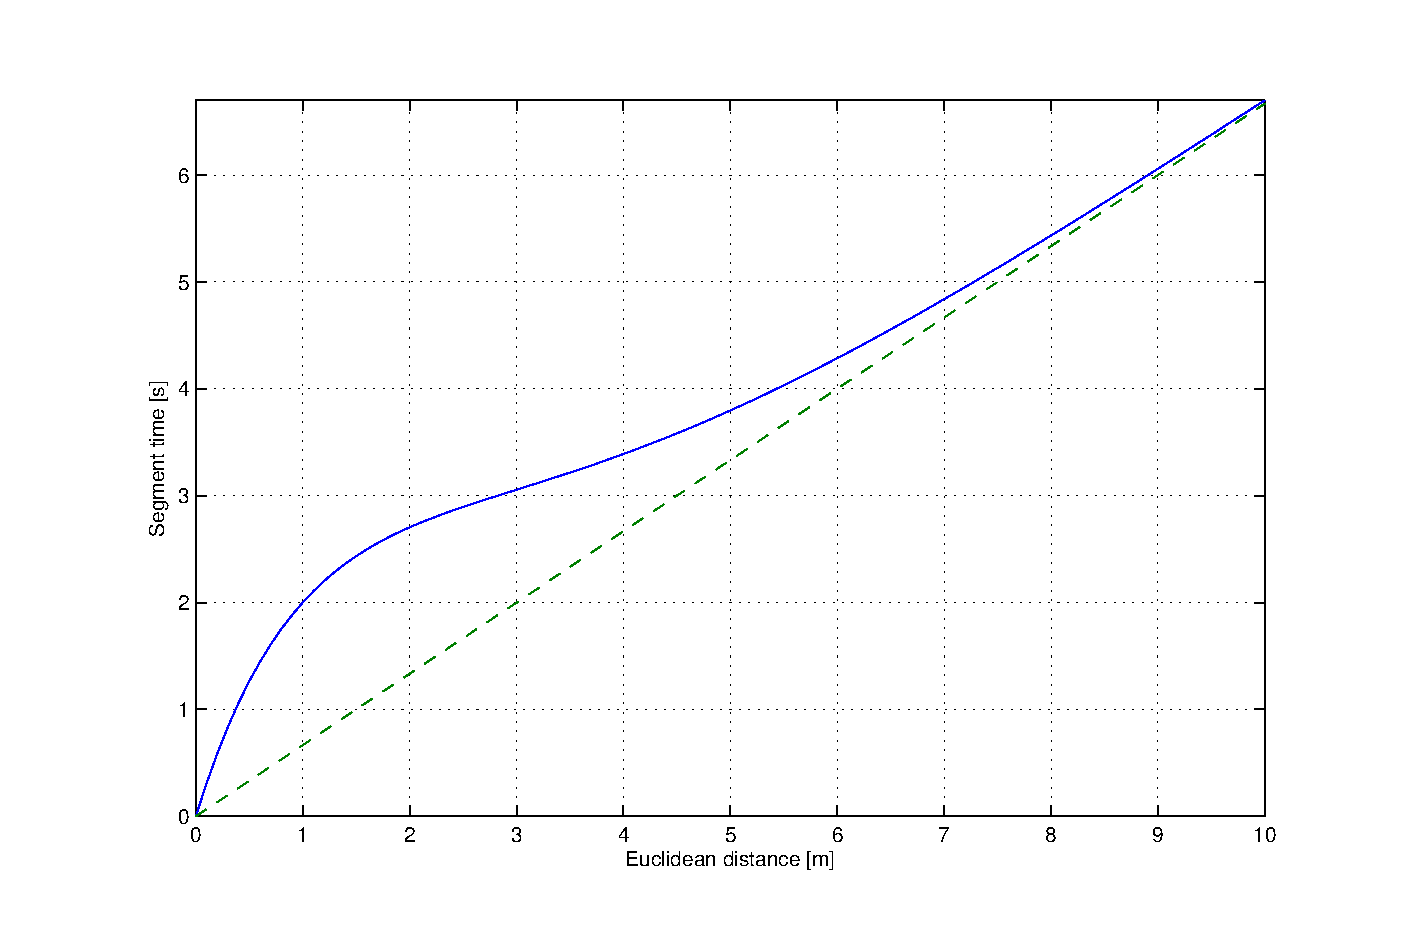
\includegraphics[trim = 20mm 10mm 20mm 10mm,width=1\textwidth]{pics/time_estimation.eps}
   \caption{The segment time $T$ depends on the Euclidean distance $d_{norm}$ of a segment as well as on the max. velocity $v_{max}$ and the max. acceleration $a_{max}$. For short segments the acceleration time is incorporated.}
   \label{pic:timeEstimation}
\end{figure}

Once the segment times are calculated, the initial snap minimized solution can be computed according to equation \ref{equ:dpstar}. The initial solution for a 3 dimensional problem with 2 segments is depict in figure \ref{pic:initialSolution}. The start of the trajectory is the origin of the Cartesian coordinate system (0/0/0). For both, start and goal state, the velocity, the acceleration, the jerk and the snap are fixed and set to zero. For all the other sampling points (vertices) the derivatives are unspecified. The Cartesian coordinates of the sampling points are chosen manually and are listed in the following table: 

\begin{table}[H] 
\begin{center}
    \begin{tabular}{ | l | c | c | c |}
    \hline
    Waypoint & x-coordinate & y-coordinate & z-coordinate\\ \hline
    Start-Vertex & 0 & 0 & 0 \\ \hline
    Vertex 1 & 1 & 2 & 5\\ \hline
    Goal-Vertex & 3 & 4 & 6\\
    \hline
    \end{tabular}
    \caption{3 manually chosen  vertices}
    \label{tab:vertices}
\end{center}
\end{table}


The initial solution depicted in figure \ref{pic:initialSolution} is divided into 3 plots. Plot a) shows the position (i.e. the Cartesian coordinates) whereby each of the 3 dimensions is depicted as a single graph. The Cartesian coordinates from the above-noted table are depicted as circles. 
Plot b) shows the velocity of the individual direction as a solid graph. Additional, the velocity in the three-dimensional space (i.e. the Euclidean norm of the velocity vector) is depicted as a dashed graph.
Plot c) depicts the acceleration in the individual directions (solid) and the acceleration in the three-dimensional space (dashed). Furthermore the limitation for velocity and acceleration ($v_{max} = 3 \frac{m}{s}$ and $a_{max} = 4 \frac{m}{s^2}$ for this problem) are depicted in plot b) resp. c) . The $x$-axis for all the 3 plots is the time. \newpage



\begin{figure}[h]
   \centering
   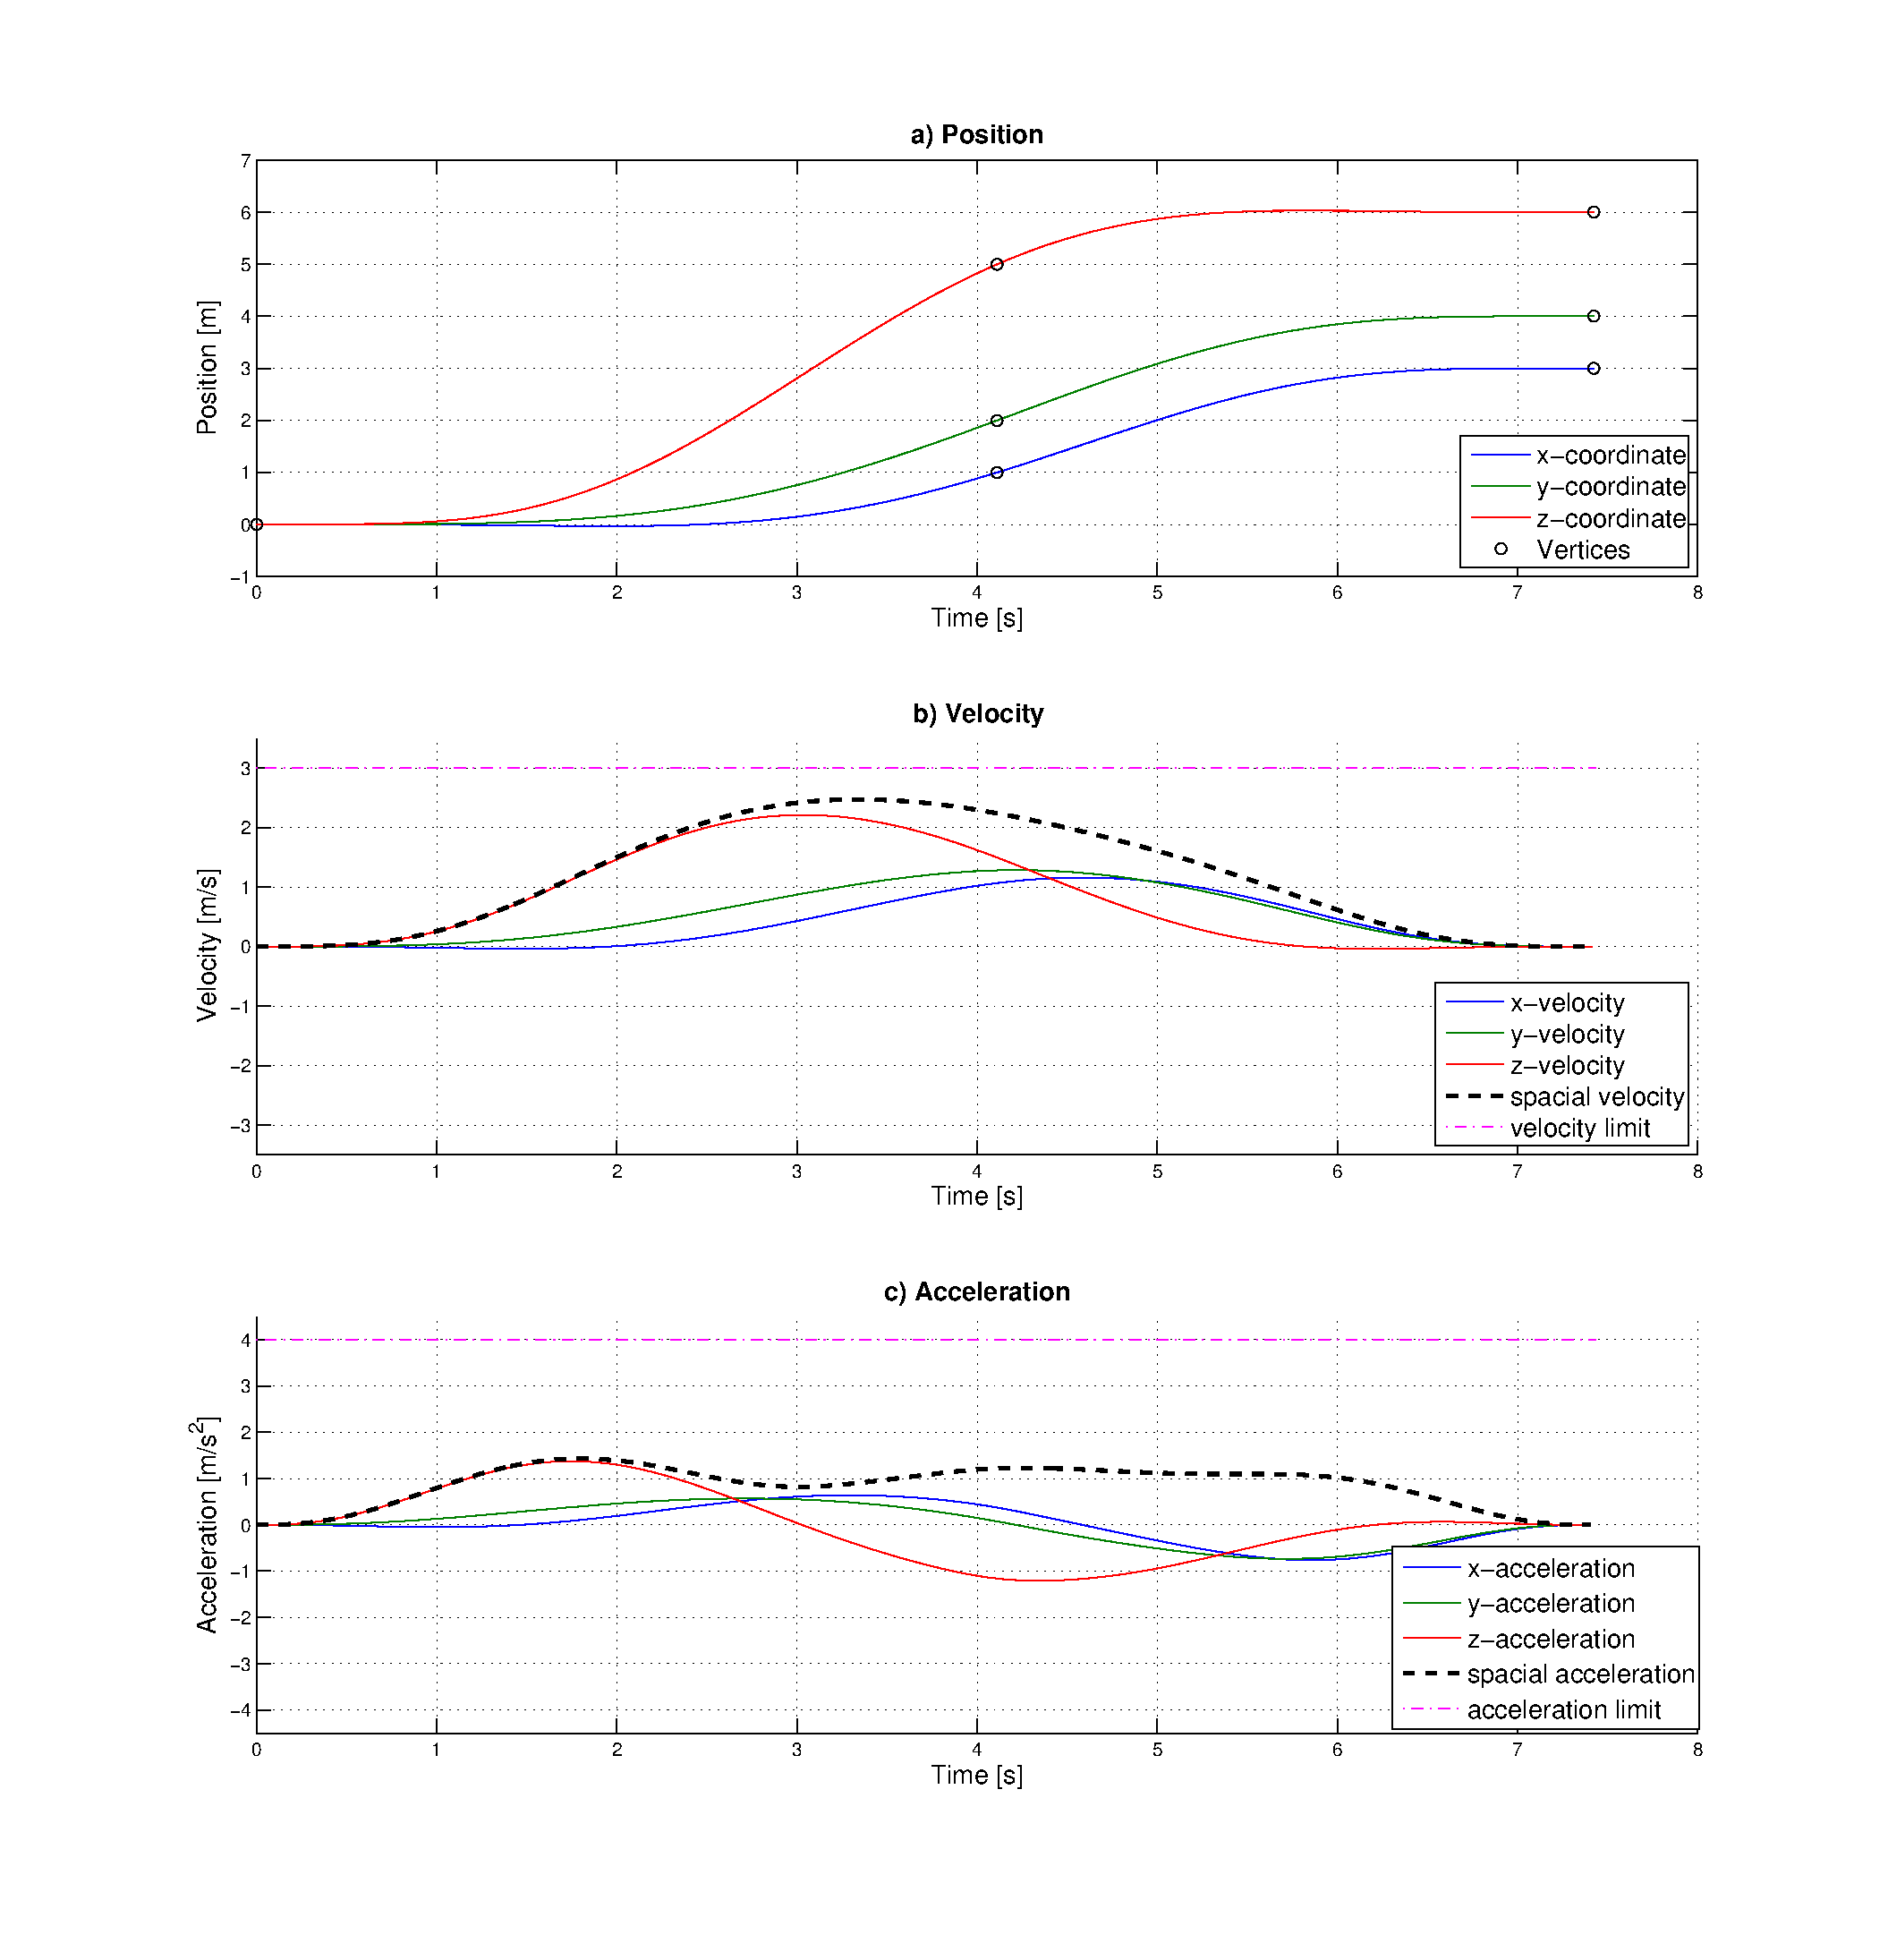
\includegraphics[trim = 35mm 30mm 30mm 15mm,clip,width=1\textwidth]{pics/2SegInit7s43.eps}
   \caption{Initial solution of a trajectory with 2 segments: Plot a) shows the position (i.e. the Cartesian coordinates). Plot b) shows the velocity and plot c) the acceleration. A dashed graph represents the velocity respectively the acceleration in the three-dimensional space.}
   \label{pic:initialSolution}
\end{figure}

As can be seen in plot b) the maximal spacial velocity is less then the user specified maximal velocity $v_{max} = 3\frac{m}{s}$. The same applies to plot c) where the maximal acceleration is far below the user specified maximal acceleration of $a_{max} = 4 \frac{m}{s^2}$. Hence, the trajectory could be more aggressive/faster without violating the limitations. \newline

\subsection{Drawbacks of the Initial Solution}\label{sec:drawbackInitial}


The individual segment times and consequently the total time of the initial trajectory are defined by equation \ref{equ:segmentTime}. Since equation \ref{equ:segmentTime} does not incorporate the circumstances from one segment to an other it is likely to find a better trajectory (i.e. a trajectory with a smaller total cost) with the same total time but a different ratio between the segment time. Moreover there is no possibility to adjust the aggressiveness of the initial solution since the segment times are calculated up front. \newline

Recapitulating, the modification of the individual segment times and therefore the modification of the ratio of the segment times can lead to a better solution. Supplementary, the modification of the individual segment times gives us the opportunity to adjust the aggressiveness of a trajectory.



\section{Time Allocation}\label{sec:penalty}

So fare, only the geometric cost (i. e. the squared snap) was included in the cost function defined in equation \ref{equ:Rxx_cost}. Minimization of the geometric cost ensures a smooth trajectory without abrupt input signal but has no effect on the aggressiveness of a trajectory. Therefore equation \ref{equ:Rxx_cost} has to be extended by the temporal cost (i.e. the sum of the segment times) which results in the total cost $J_{total}$

\begin{equation}
J_{total} =
\begin{bmatrix}
   d_f \\
  d_p
\end{bmatrix}^T
\begin{bmatrix}
   R_{ff} & R_{fp} \\
  R_{pf} & R_{pp}
\end{bmatrix}
\begin{bmatrix}
   d_f \\
  d_p
\end{bmatrix}
+ k_T \cdot \sum_{i=1}^N T_i
\label{equ:total_cost}
\end{equation}

where $k_T$ is a user specified weighting factor and $T_i$ is the segment time of the $i^{th}$ segment. \newline

A hight value for $k_T$ lays weight to the temporal cost and therefore leads to a trajectory with a brief total trajectory time. A small value for $k_T$ on the other hand lays little weight on the temporal cost, meaning the geometric cost gets more important. Since the geometric cost (i.e. the quadratic snap) decreases for long segment times with little changes in jerk, this leads to a trajectory with a long total trajectory time. Thus, the user specified weighting factor $k_T$ enables the adjustment of the aggressiveness of a trajectory. \newline

\subsection{Nonlinear Optimization}\label{sec:nonlinearopt}

The geometric cost function in equation \ref{equ:Rxx_cost} has only the unspecified endpoint derivatives $d_p$ as optimization variables. This optimization problem can be solved analytically as performed in equation \ref{equ:dpstar}. The cost function in equation \ref{equ:total_cost} has the segment times $T_i$ as additional optimization variables. Meaning the segment times $T_i$ are directly represented in the cost function and not only indirectly via the Hessian matrices $Q_{T_i}$. Since the segment times are now optimization variables, the Hessian matrices $Q_{T_i}$ are no longer defined in advance and the problem cannot be solved analytically. Due to that a nonlinear solver is used. In this master thesis NLopt, a open-source library for nonlinear optimization, is applied. The unspecified endpoint derivatives $d_p$ and the segment times $T_i$ of the initial solution are the initial values for the nonlinear solver. Meaning, the initial solution has to be computed in advance to start a nonlinear optimization \newline

To illustrate the nonlinear optimization the trajectory with the same 3 vertices (defined in the table  \ref{tab:vertices}) is reused. In this master thesis position, velocity, acceleration, jerk and snap are fixed for the start and for the goal vertex since we want to start from complete rest and want to end up in standstill. For the vertex in the middle the position is fixed but velocity, acceleration, jerk and snap are unspecified, resulting in the first 4 optimization variables. Since this is a 3 dimensional problem, the number of geometric optimization variables triple to 12. Together with the segment time of the two segments, the problem ends up with a total number of 14 optimization variables. \pagebreak 

%The influence of the number of optimization varibales on the performance is discussed in section: TODO \newline

The result of the nonlinear optimization is depicted in figure \ref{pic:optimizedSolution}. Plot a) depicts the position (i.e. the Cartesian coordinates) whereby each of the 3 dimensions is depicted as a single graph. Plot b) shows the velocity of the individual direction as a solid graph. Additional, the velocity in the three-dimensional space (i.e. the Euclidean norm of the velocity vector) is depicted as a dashed graph. Plot c) depicts the acceleration in the individual directions (solid) and the acceleration in the three-dimensional space (dashed). Furthermore the limitation ($v_{max} = 3 \frac{m}{s}$ and $a_{max} = 4 \frac{m}{s^2}$ for this problem) are depicted.
%\vspace*{3\baselineskip}

\begin{figure}[h]
   \centering
   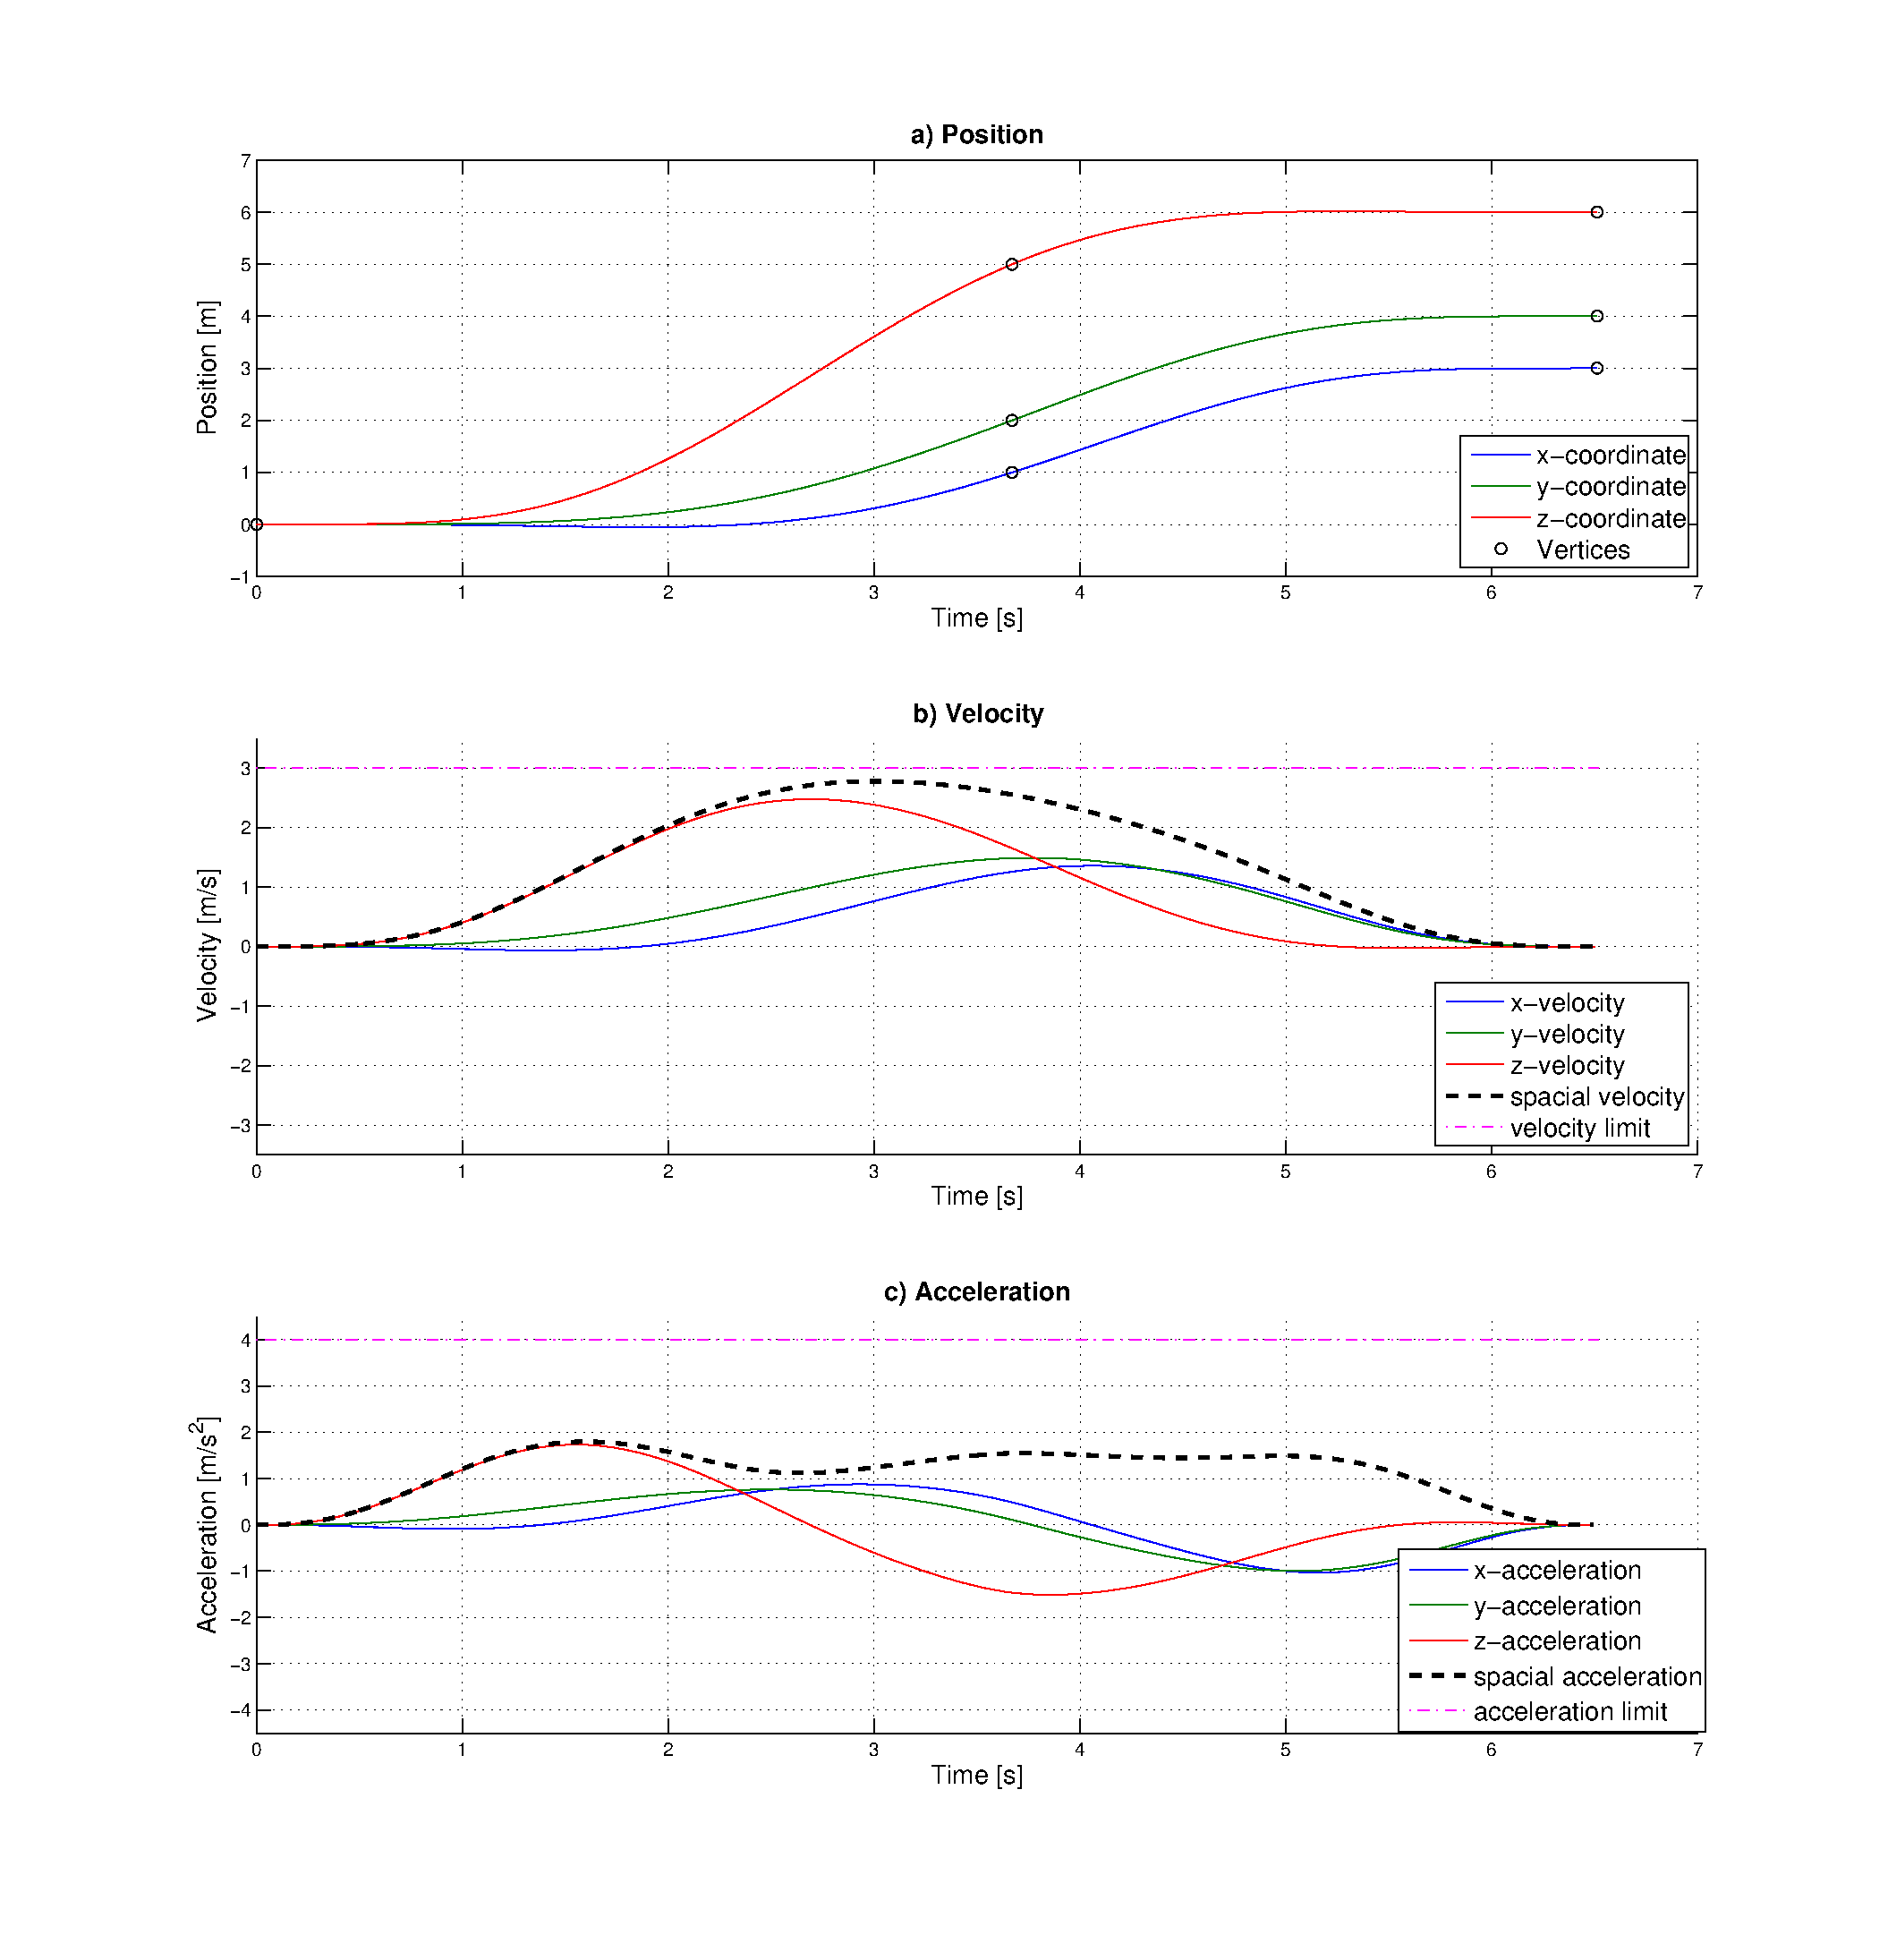
\includegraphics[trim = 35mm 20mm 30mm 8mm,clip,width=1\textwidth]{pics/2SegOpti6s52k100.eps}
   \caption{Optimized solution of a trajectory with 2 segments: Plot a) shows the position (i.e. the Cartesian coordinates). Plot b) shows the velocity and plot c) the acceleration. A dashed graph represents the velocity respectively the acceleration in the three-dimensional space. Weighting factor $k_T$ was set to 100.}
   \label{pic:optimizedSolution}
\end{figure}



As can be seen in figure \ref{pic:optimizedSolution} a) the trajectory passes the same vertices as in figure \ref{pic:initialSolution}. 
In this optimization the user specified weighting factor was set to $k_T = 100$. This rather small value for $k_T$ leads to a trajectory which is neither affected by the limitation on the velocity (the spacial velocity in plot b) is always below the velocity limit) nor by the limitation on acceleration(the spacial acceleration in plot c) is always below the acceleration limit). Nevertheless, the optimized trajectory with a duration of $6.52 s$ is faster then the initial solution with a duration of $7.43 s$.\newline

To get a more aggressive trajectory the value for $k_T$ has to be increased. In figure \ref{pic:optimizedSolution2k190} the optimize trajectory for $k_T = 190$ is depicted. As can be seen in plot b) the limitation on the velocity comes into play, i.e. the spacial velocity is restricted to $v_{max} = 3 \frac{m}{s}$. The duration of the trajectory depicted in figure \ref{pic:optimizedSolution2k190} is $6.01s$. Although the maximal velocity and the maximal acceleration are higher than in figure \ref{pic:optimizedSolution}, the pathway of the spacial velocity and of the spacial acceleration look very similar for $k_T = 100$ and $k_T = 190$.
%\vspace*{3\baselineskip}

\begin{figure}[H]
   \centering
   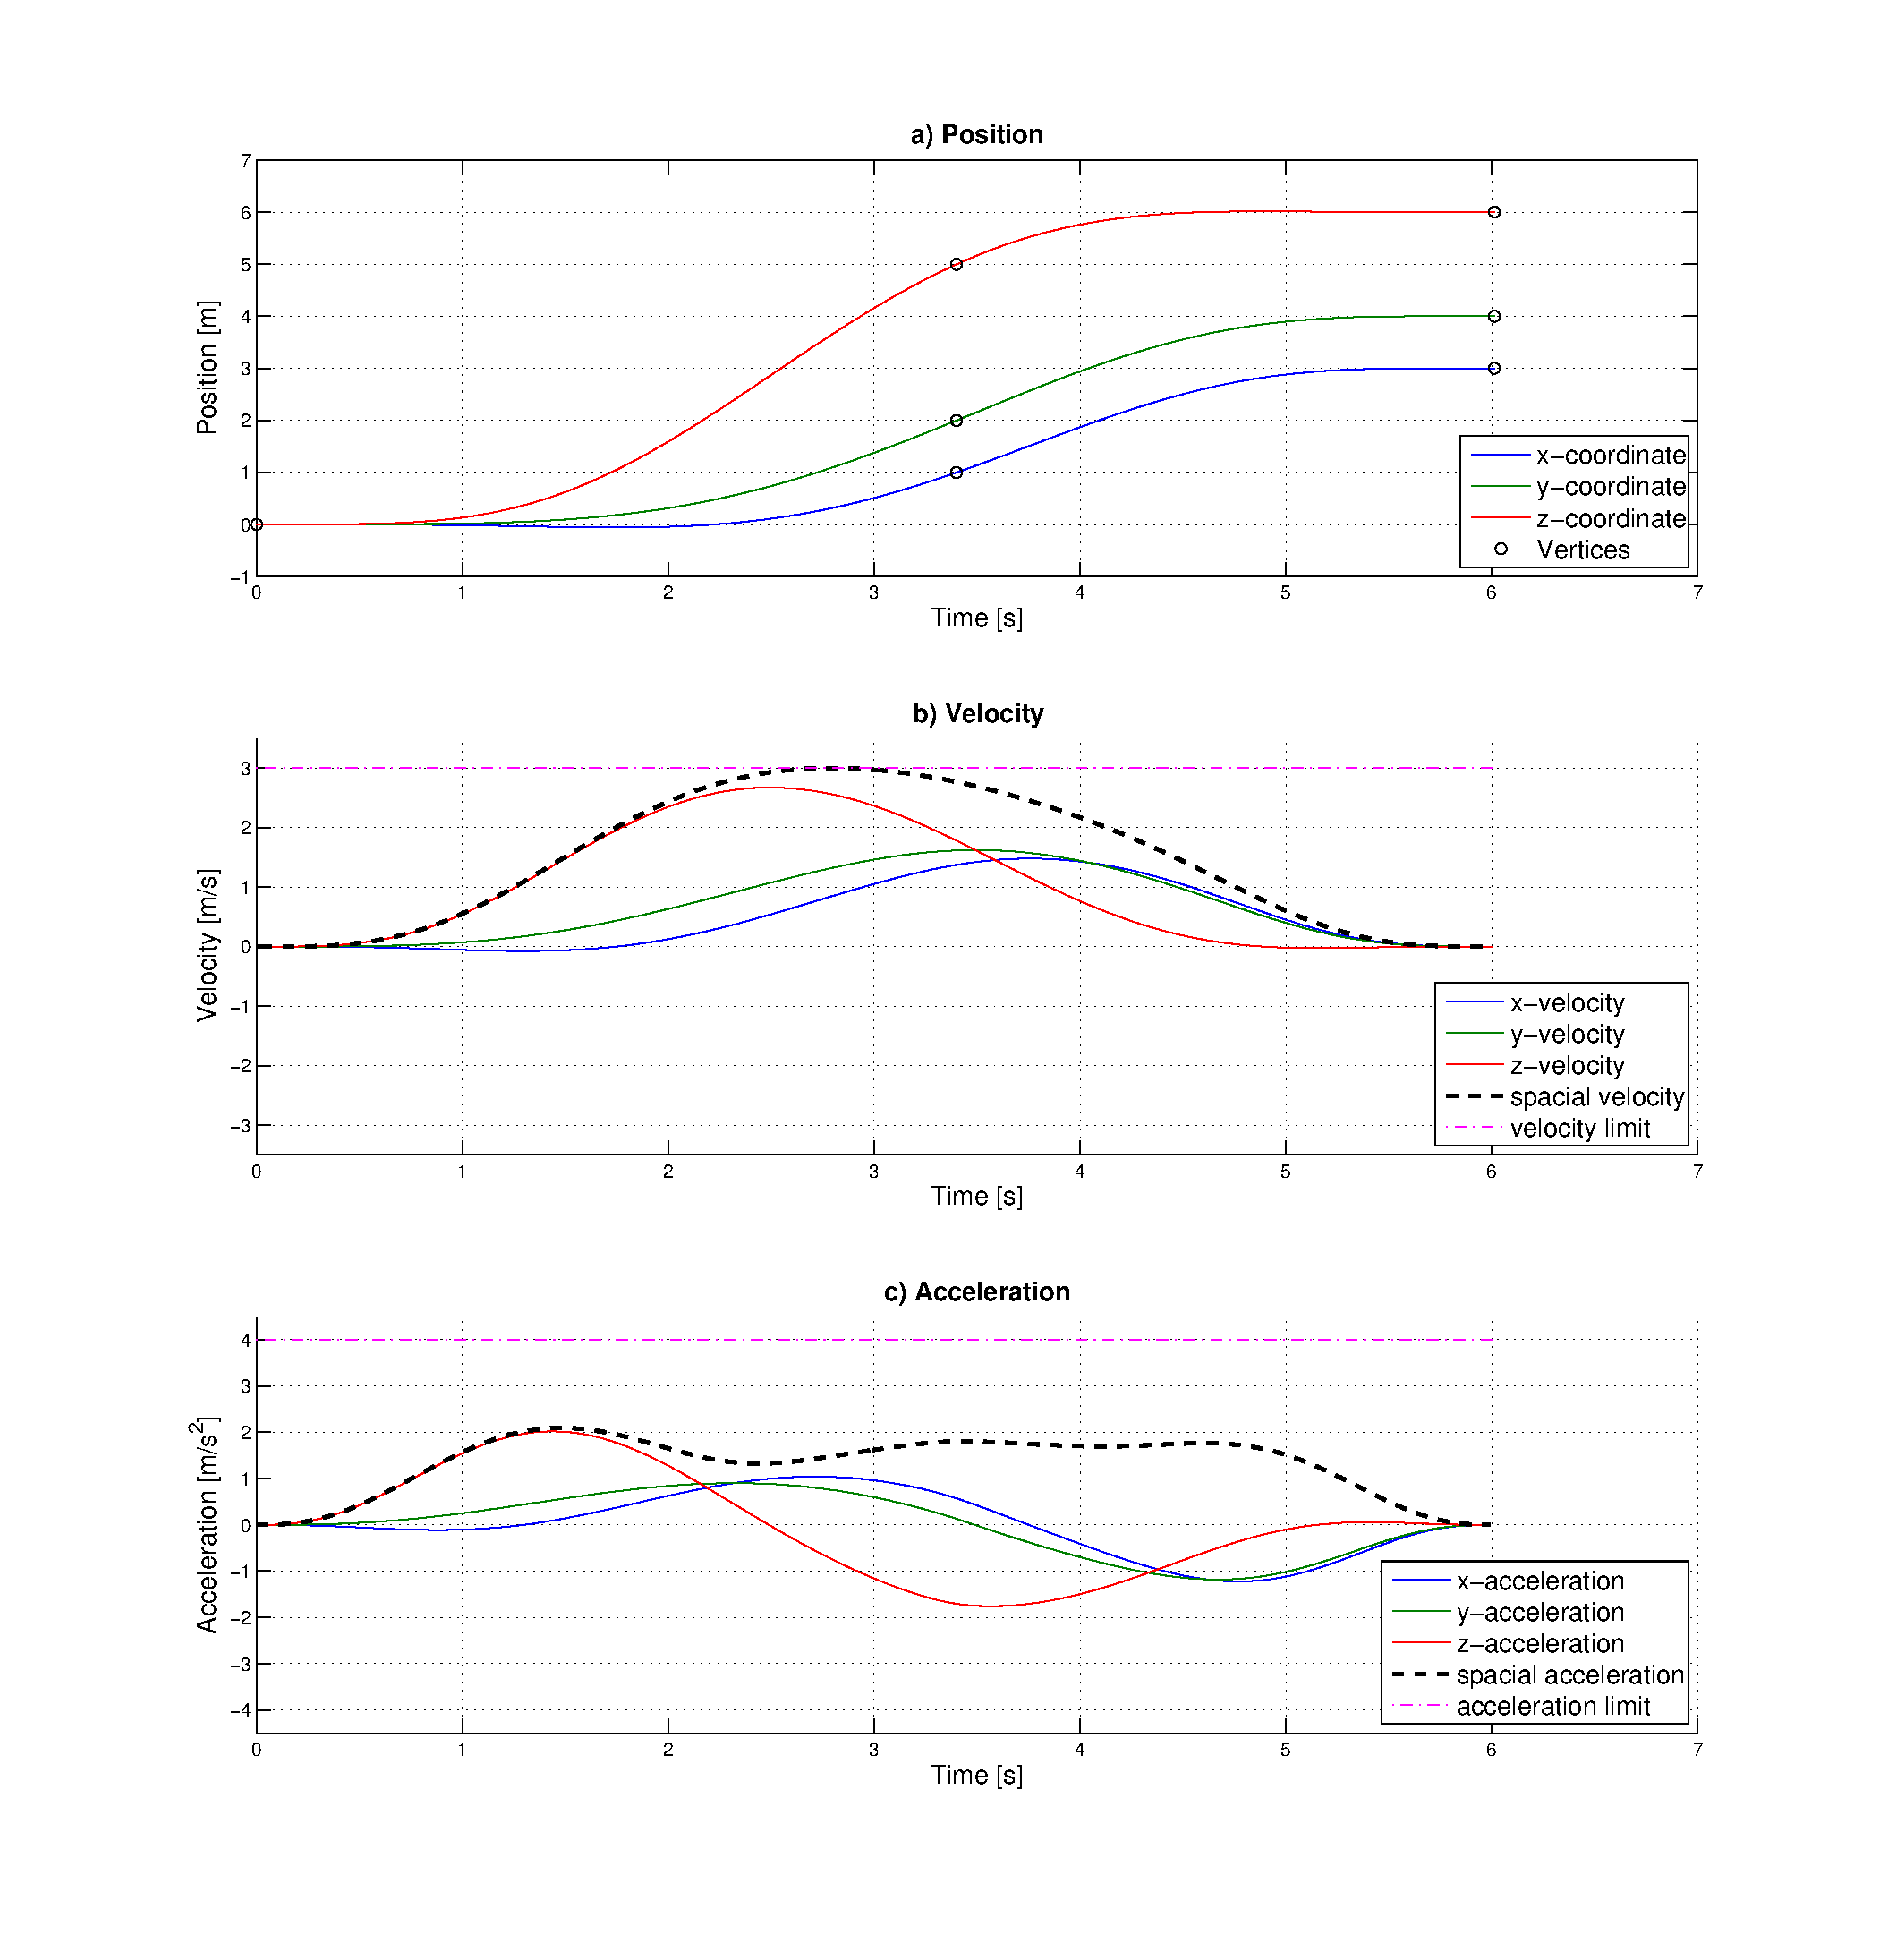
\includegraphics[trim = 35mm 20mm 30mm 15mm,clip,width=1\textwidth]{pics/2SegOpti6s01k190.eps}
   \caption{Optimized solution of a trajectory with 2 segments: Plot a) shows the position (i.e. the Cartesian coordinates). Plot b) shows the velocity and plot c) the acceleration. A dashed graph represents the velocity respectively the acceleration in the three-dimensional space. Weighting factor $k_T$ was set to 190.}
   \label{pic:optimizedSolution2k190}
\end{figure}


In a next step the value for $k_T$ is increased even more and set to $k_T = 2000$. The resulting trajectory is depicted in figure \ref{pic:optimizedSolution2k2000}. The duration of this aggressive trajectory is $5.16s$. The pathway of the spacial velocity looks now different than in the previous figures. The spacial velocity not only touches the velocity limit but stays at the limit for circa one second.
%\vspace*{3.2\baselineskip}

\begin{figure}[H]
   \centering
   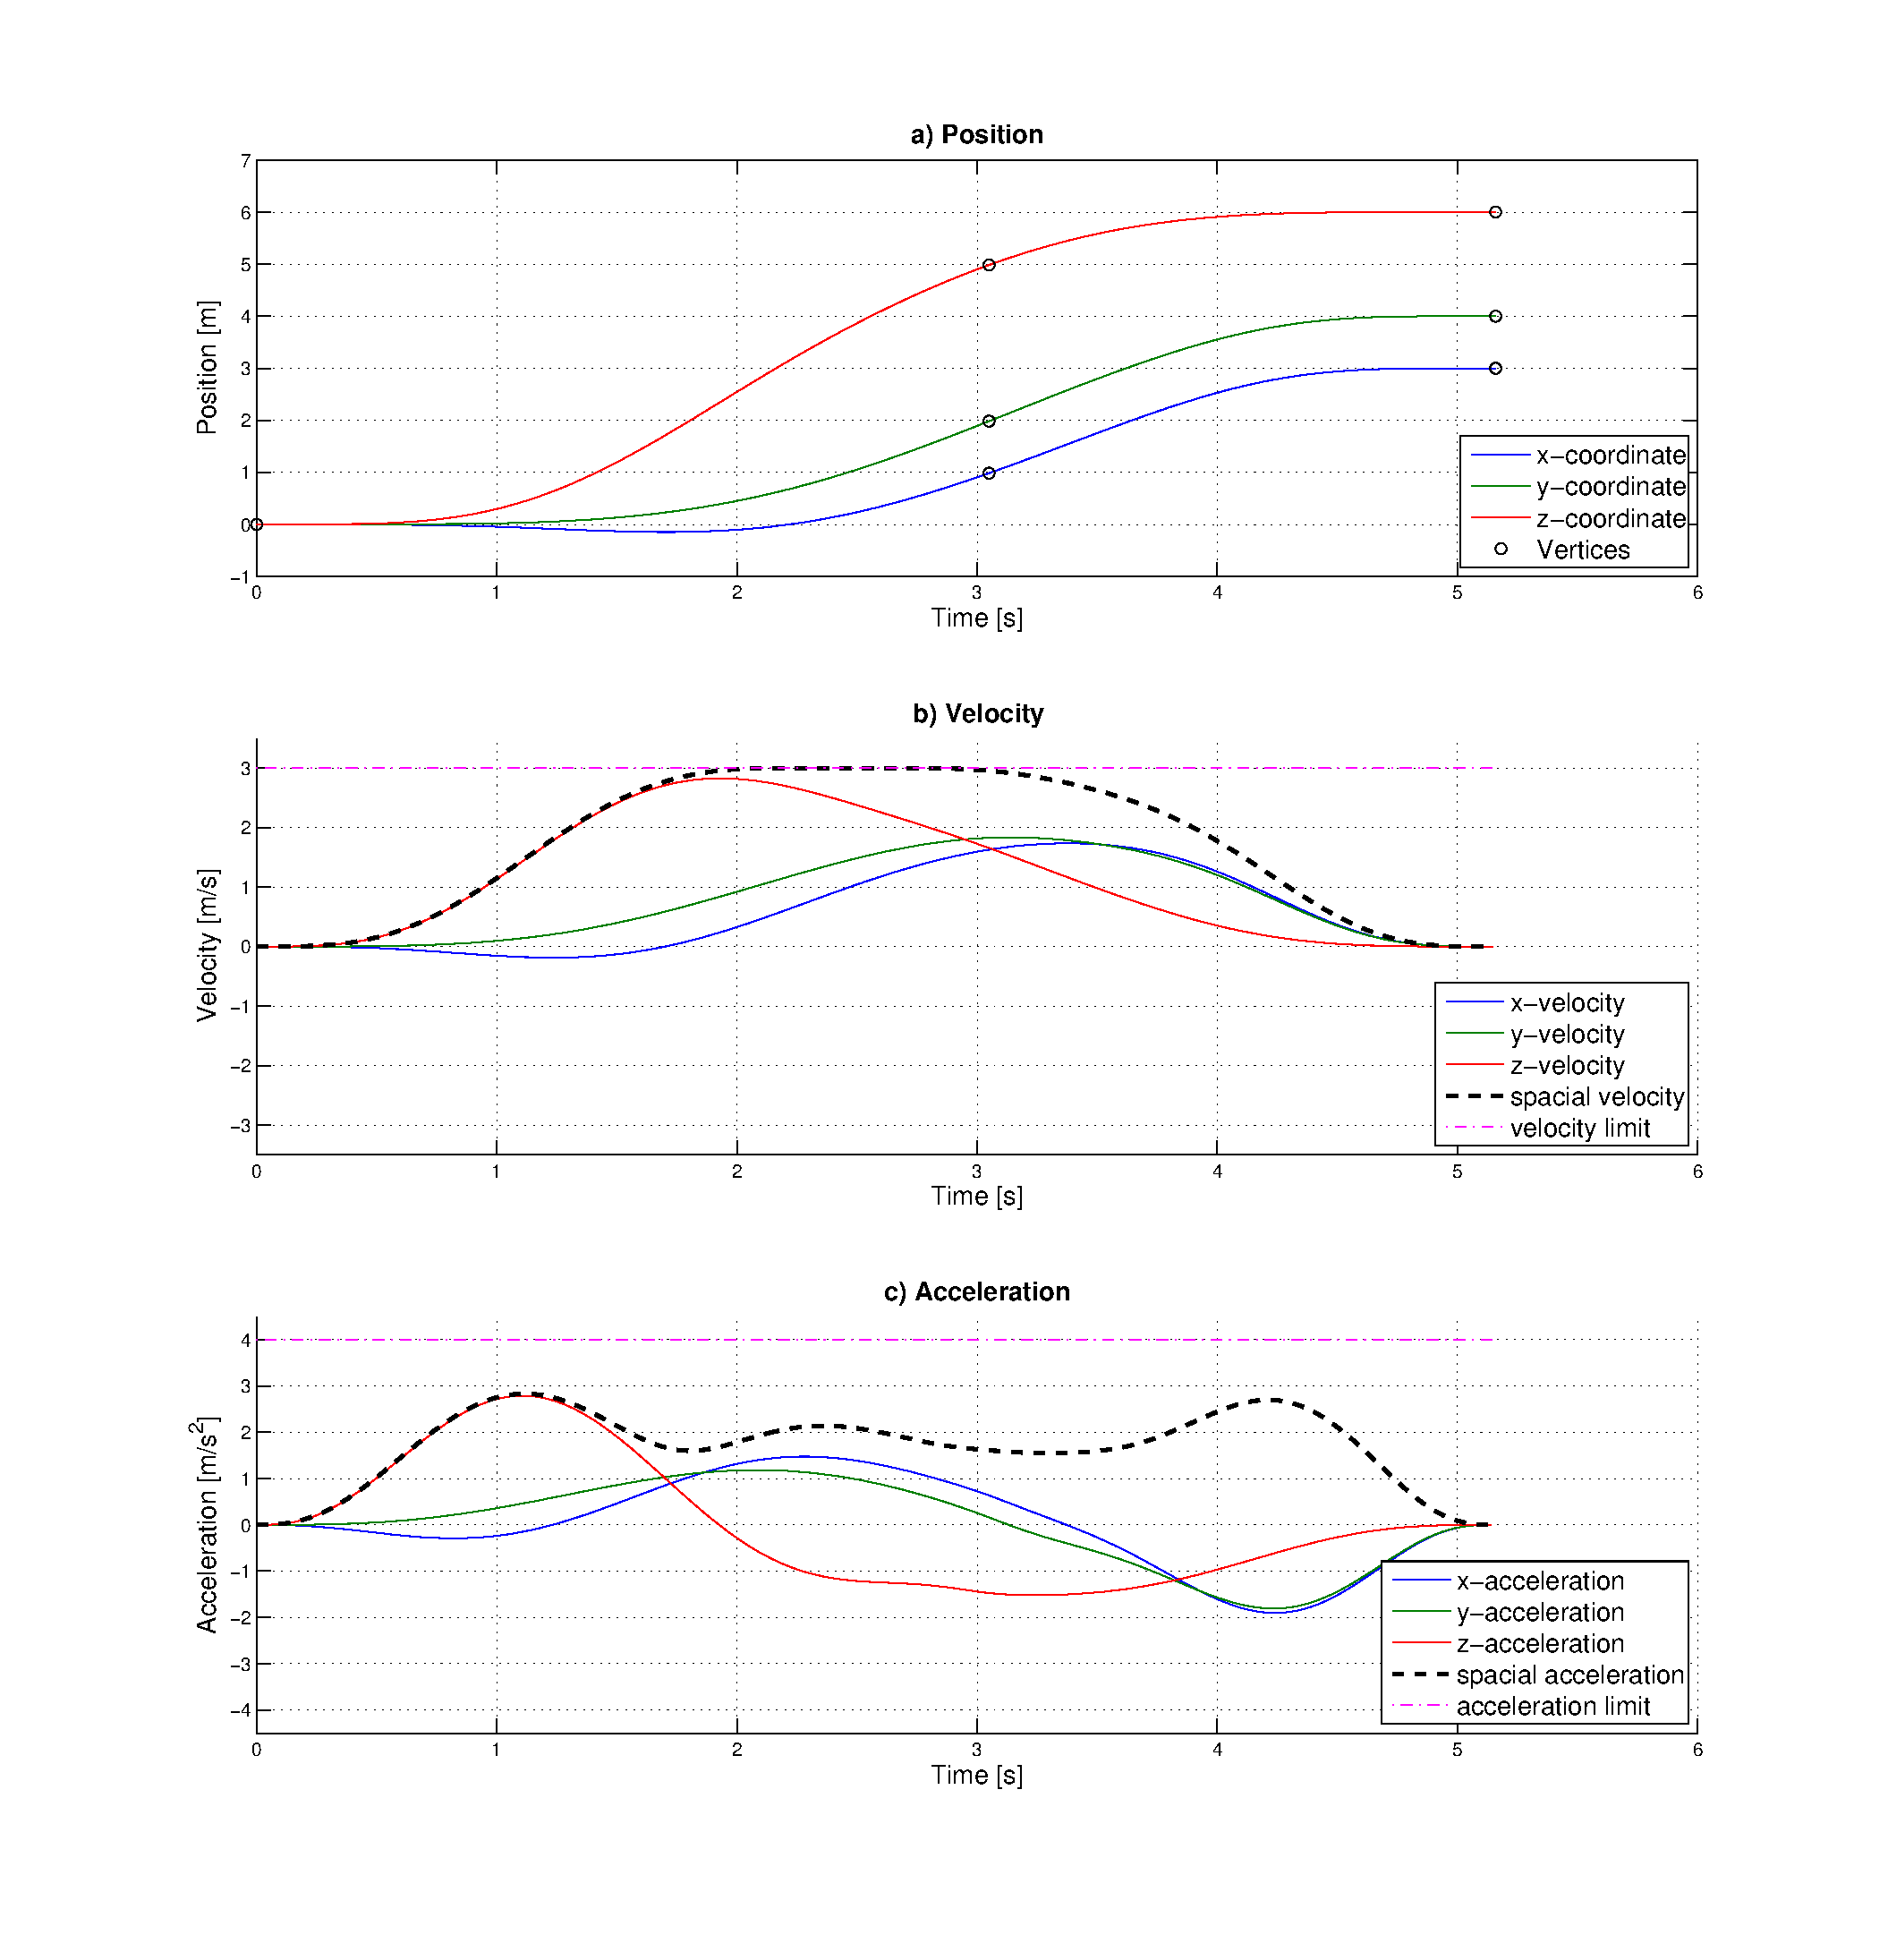
\includegraphics[trim = 35mm 30mm 30mm 15mm,clip,width=1\textwidth]{pics/2SegOpti5s16k2000.eps}
   \caption{Optimized solution of a trajectory with 2 segments: Plot a) shows the position (i.e. the Cartesian coordinates). Plot b) shows the velocity and plot c) the acceleration. A dashed graph represents the velocity respectively the acceleration in the three-dimensional space. Weighting factor $k_T$ was set to 2000.}
   \label{pic:optimizedSolution2k2000}
\end{figure}


Although figure \ref{pic:optimizedSolution2k2000} depicts a aggressive trajectory the spacial acceleration always remains under the acceleration limit. Of course this depends on the choice of the acceleration limit, i.e. the acceleration limit would get significant if $a_{max}$ is set to less than $3 \frac{m}{s^2}$.
A factor which is independent from the user specified choice of $k_T$ is the pathway of the trajectory. For a trajectory with little curves the acceleration has a smaller influence on the duration than the velocity. Since the coordinates in all 3 dimensions increases permanently this is the case in figure \ref{pic:optimizedSolution2k2000}. \newline



To depict the features of a trajectory with more curves an other set of vertices is chosen:

\begin{table}[H] 
\begin{center}
    \begin{tabular}{ | l | c | c | c |}
    \hline
    Waypoint & x-coordinate & y-coordinate & z-coordinate\\ \hline
    Start-Vertex & 0 & 0 & 0 \\ \hline
    Vertex 1 & 5 & 1 & -2\\ \hline
   Vertex 2 & 3 & -2 & 1\\ \hline
   Vertex 3 & -1 & 2 & 3\\ \hline
    Goal-Vertex & 1 & -1 & -2\\
    \hline
    \end{tabular}
\caption{5 manually chosen  vertices}
    \label{tab:5vertices}
\end{center}
\end{table}


The initial solution with 4 segments passing through  the above-noted vertices is depicted in figure \ref{pic:optimizedSolution4init}. 
%\vspace*{4\baselineskip}

\begin{figure}[H]
   \centering
   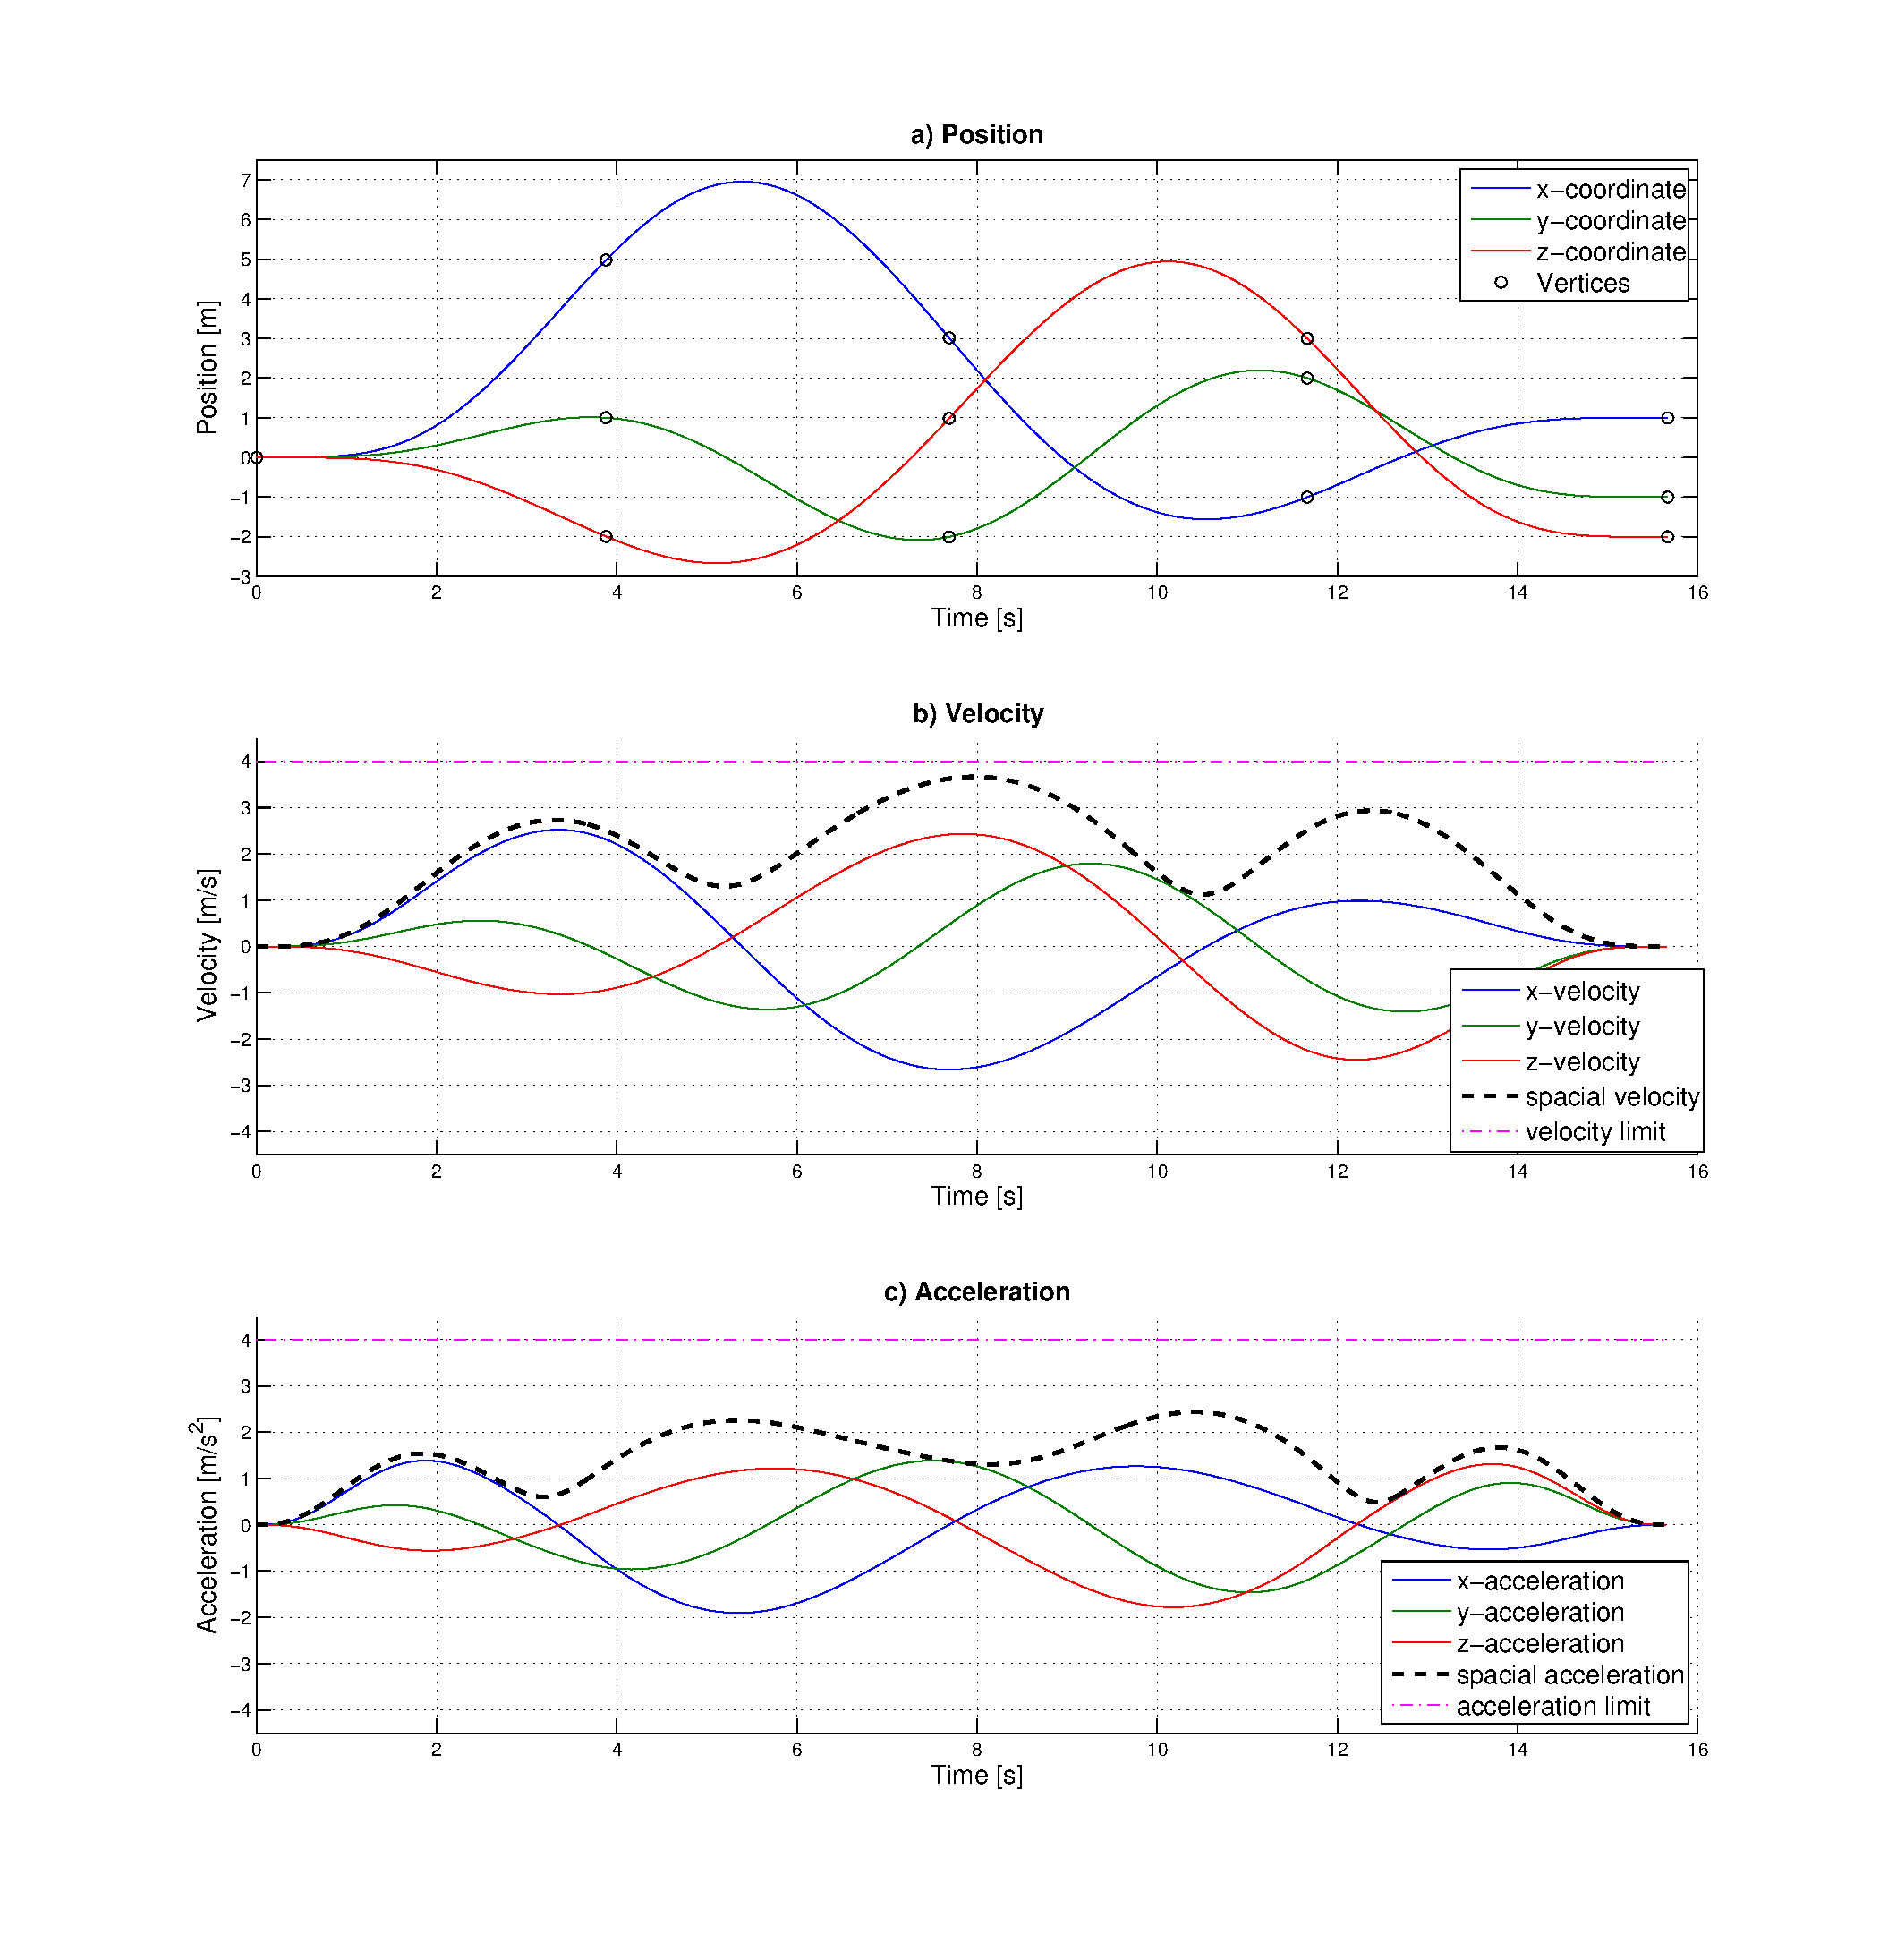
\includegraphics[trim = 35mm 30mm 30mm 15mm,clip,width=1\textwidth]{pics/4SegInit15s67.eps}
   \caption{Initial solution of a trajectory with 4 segments: A dashed graph represents the velocity respectively the acceleration in the three-dimensional space.}
   \label{pic:optimizedSolution4init}
\end{figure}
\newpage

The initial solution is required to define the initial values of the nonlinear optimization.
As can be seen in plot b) and plot c) neither the limitation on the velocity nor the limitation on the acceleration are violated.

%\begin{figure}[h]
%   \centering
%   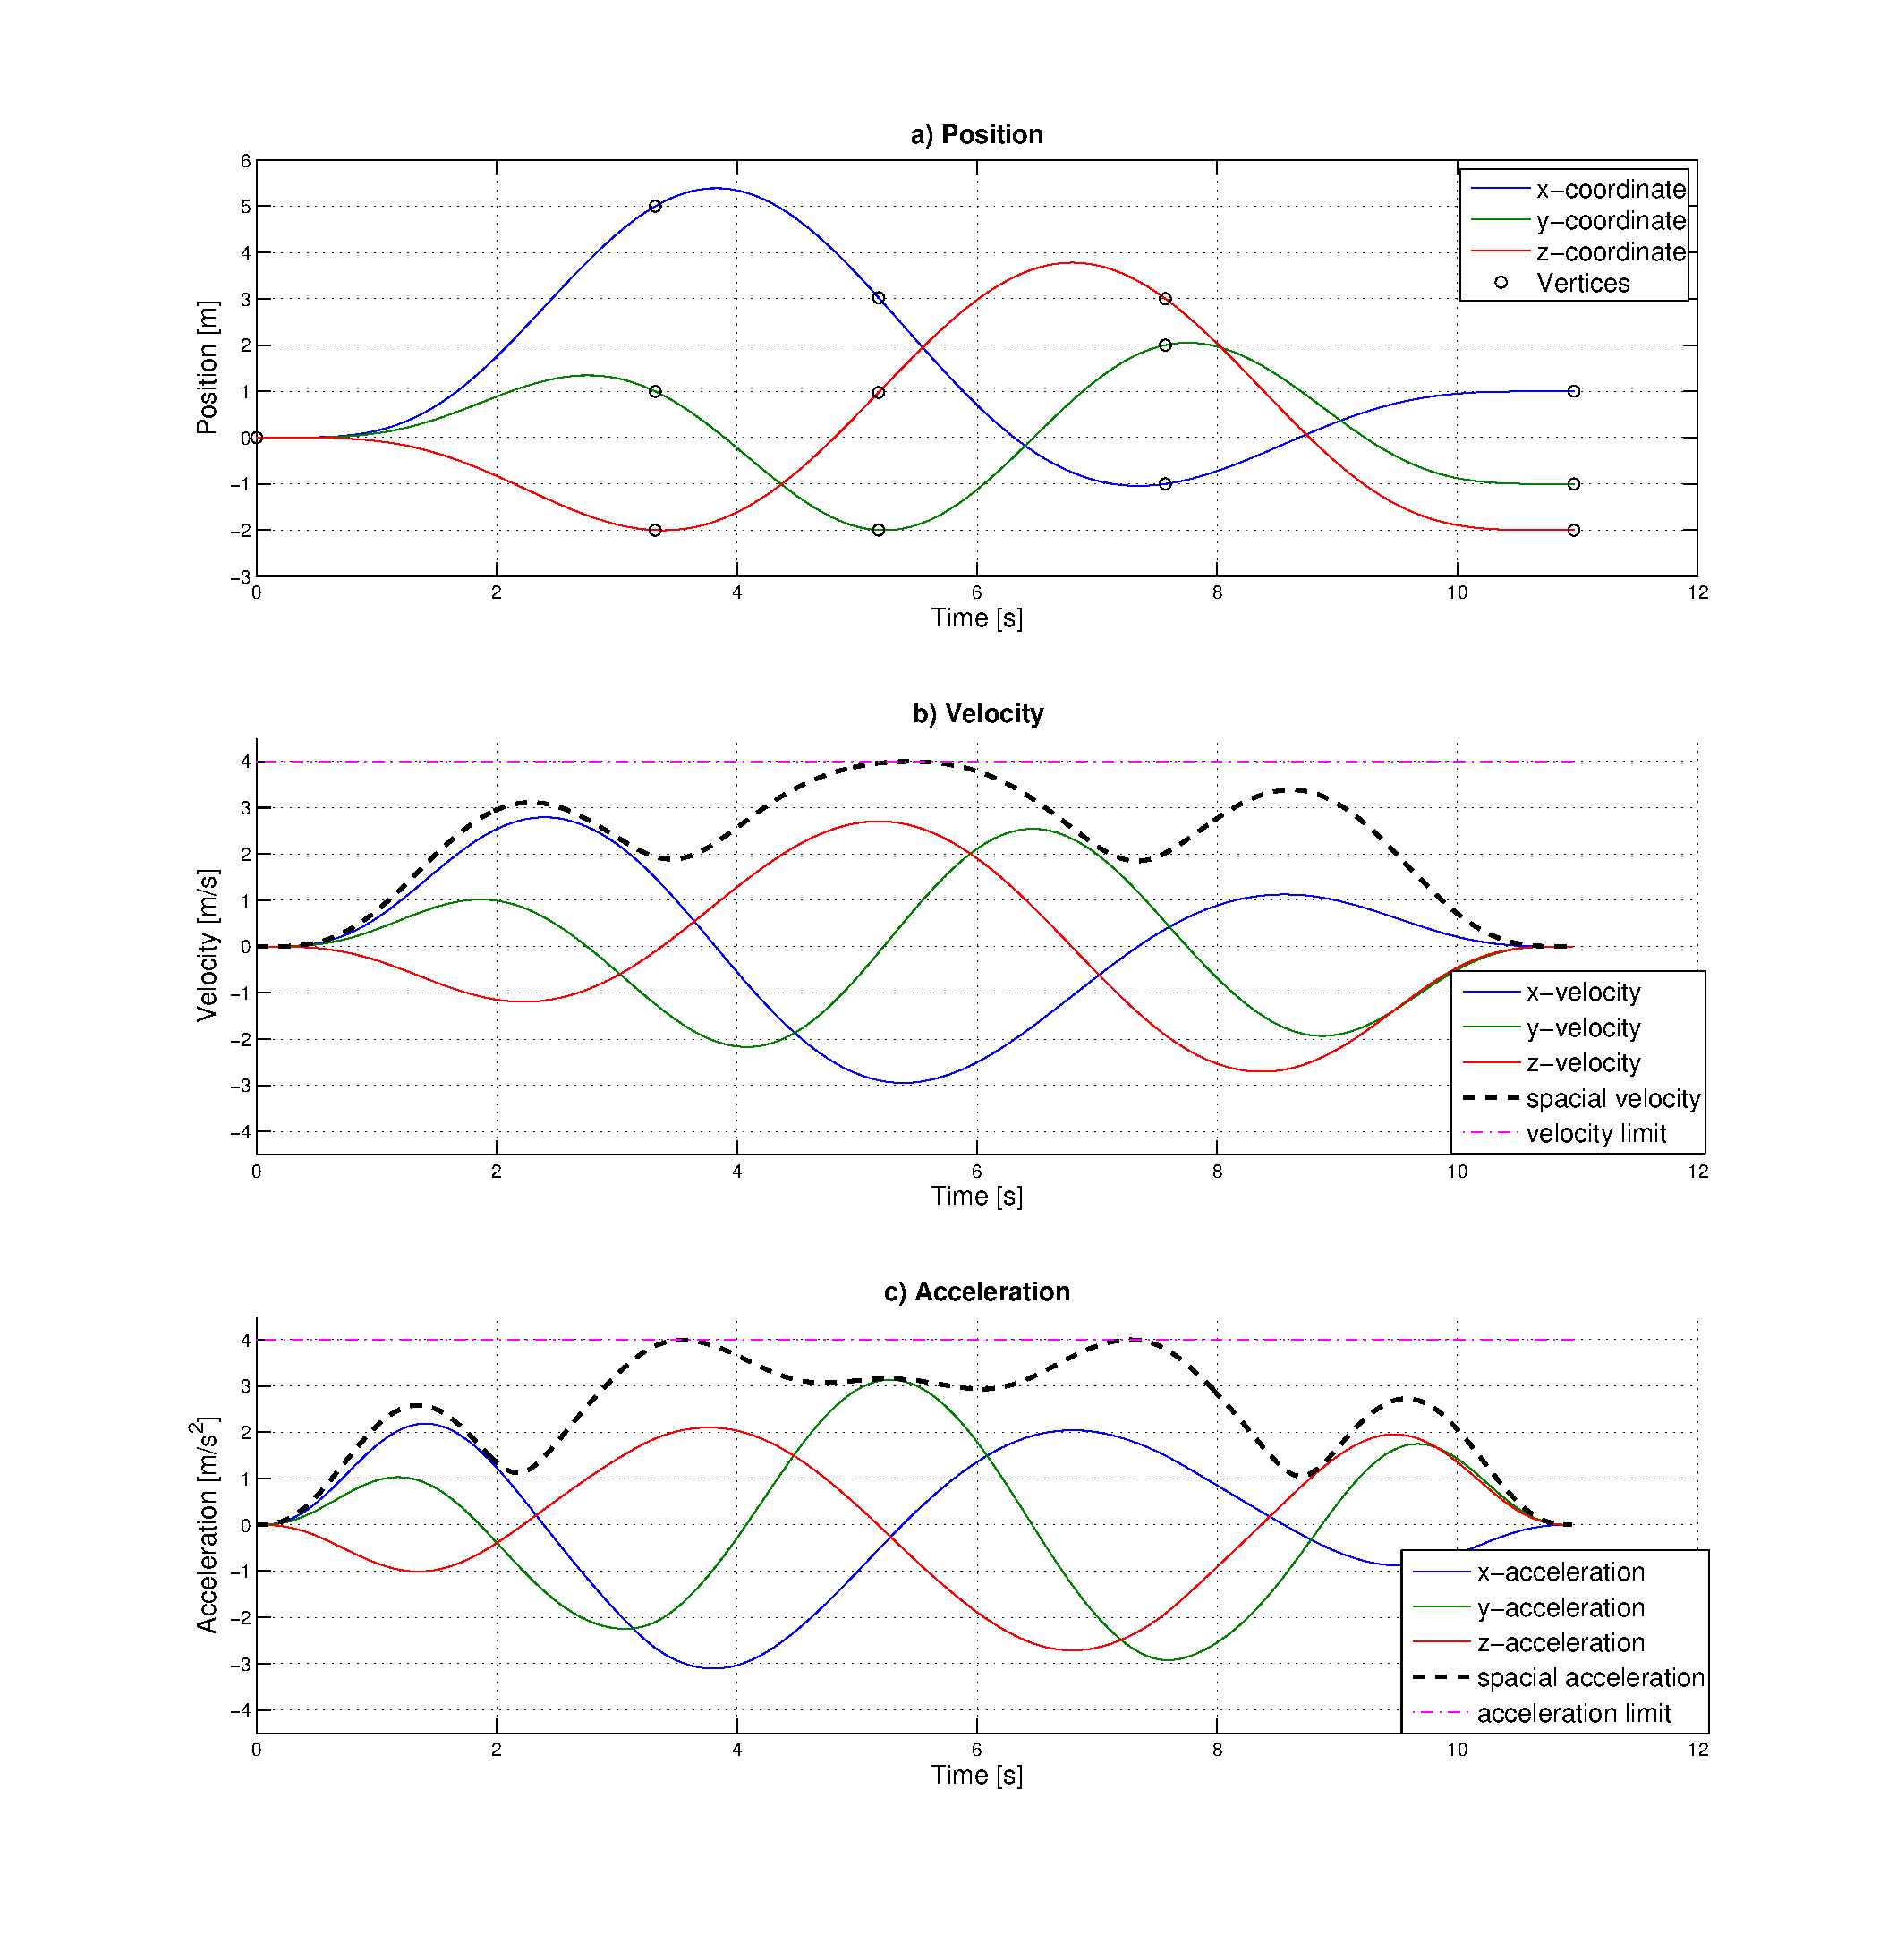
\includegraphics[trim = 35mm 20mm 30mm 35mm,width=1\textwidth]{pics/4SegOpti10s97k400.eps}
%   \caption{...................................................................................... ..... ............. . . . . ...................... ......... .........}
%\end{figure}


Using the unspecified enpoint derivatives $d_P$ and the segment times $T_i$ of the initial solution as initial values for the optimization variables the nonlinear optimization was performed with a weighting factor of $k_T = 2000$. The optimized trajectory is depicted in figure \ref{pic:optimizedSolution4optik2000}. The duration of the optimized trajectory is $10.02s$ whereas the duration of the initial trajectory depicted in figure \ref{pic:optimizedSolution4init} is $15.67s$.


\begin{figure}[H]
   \centering
   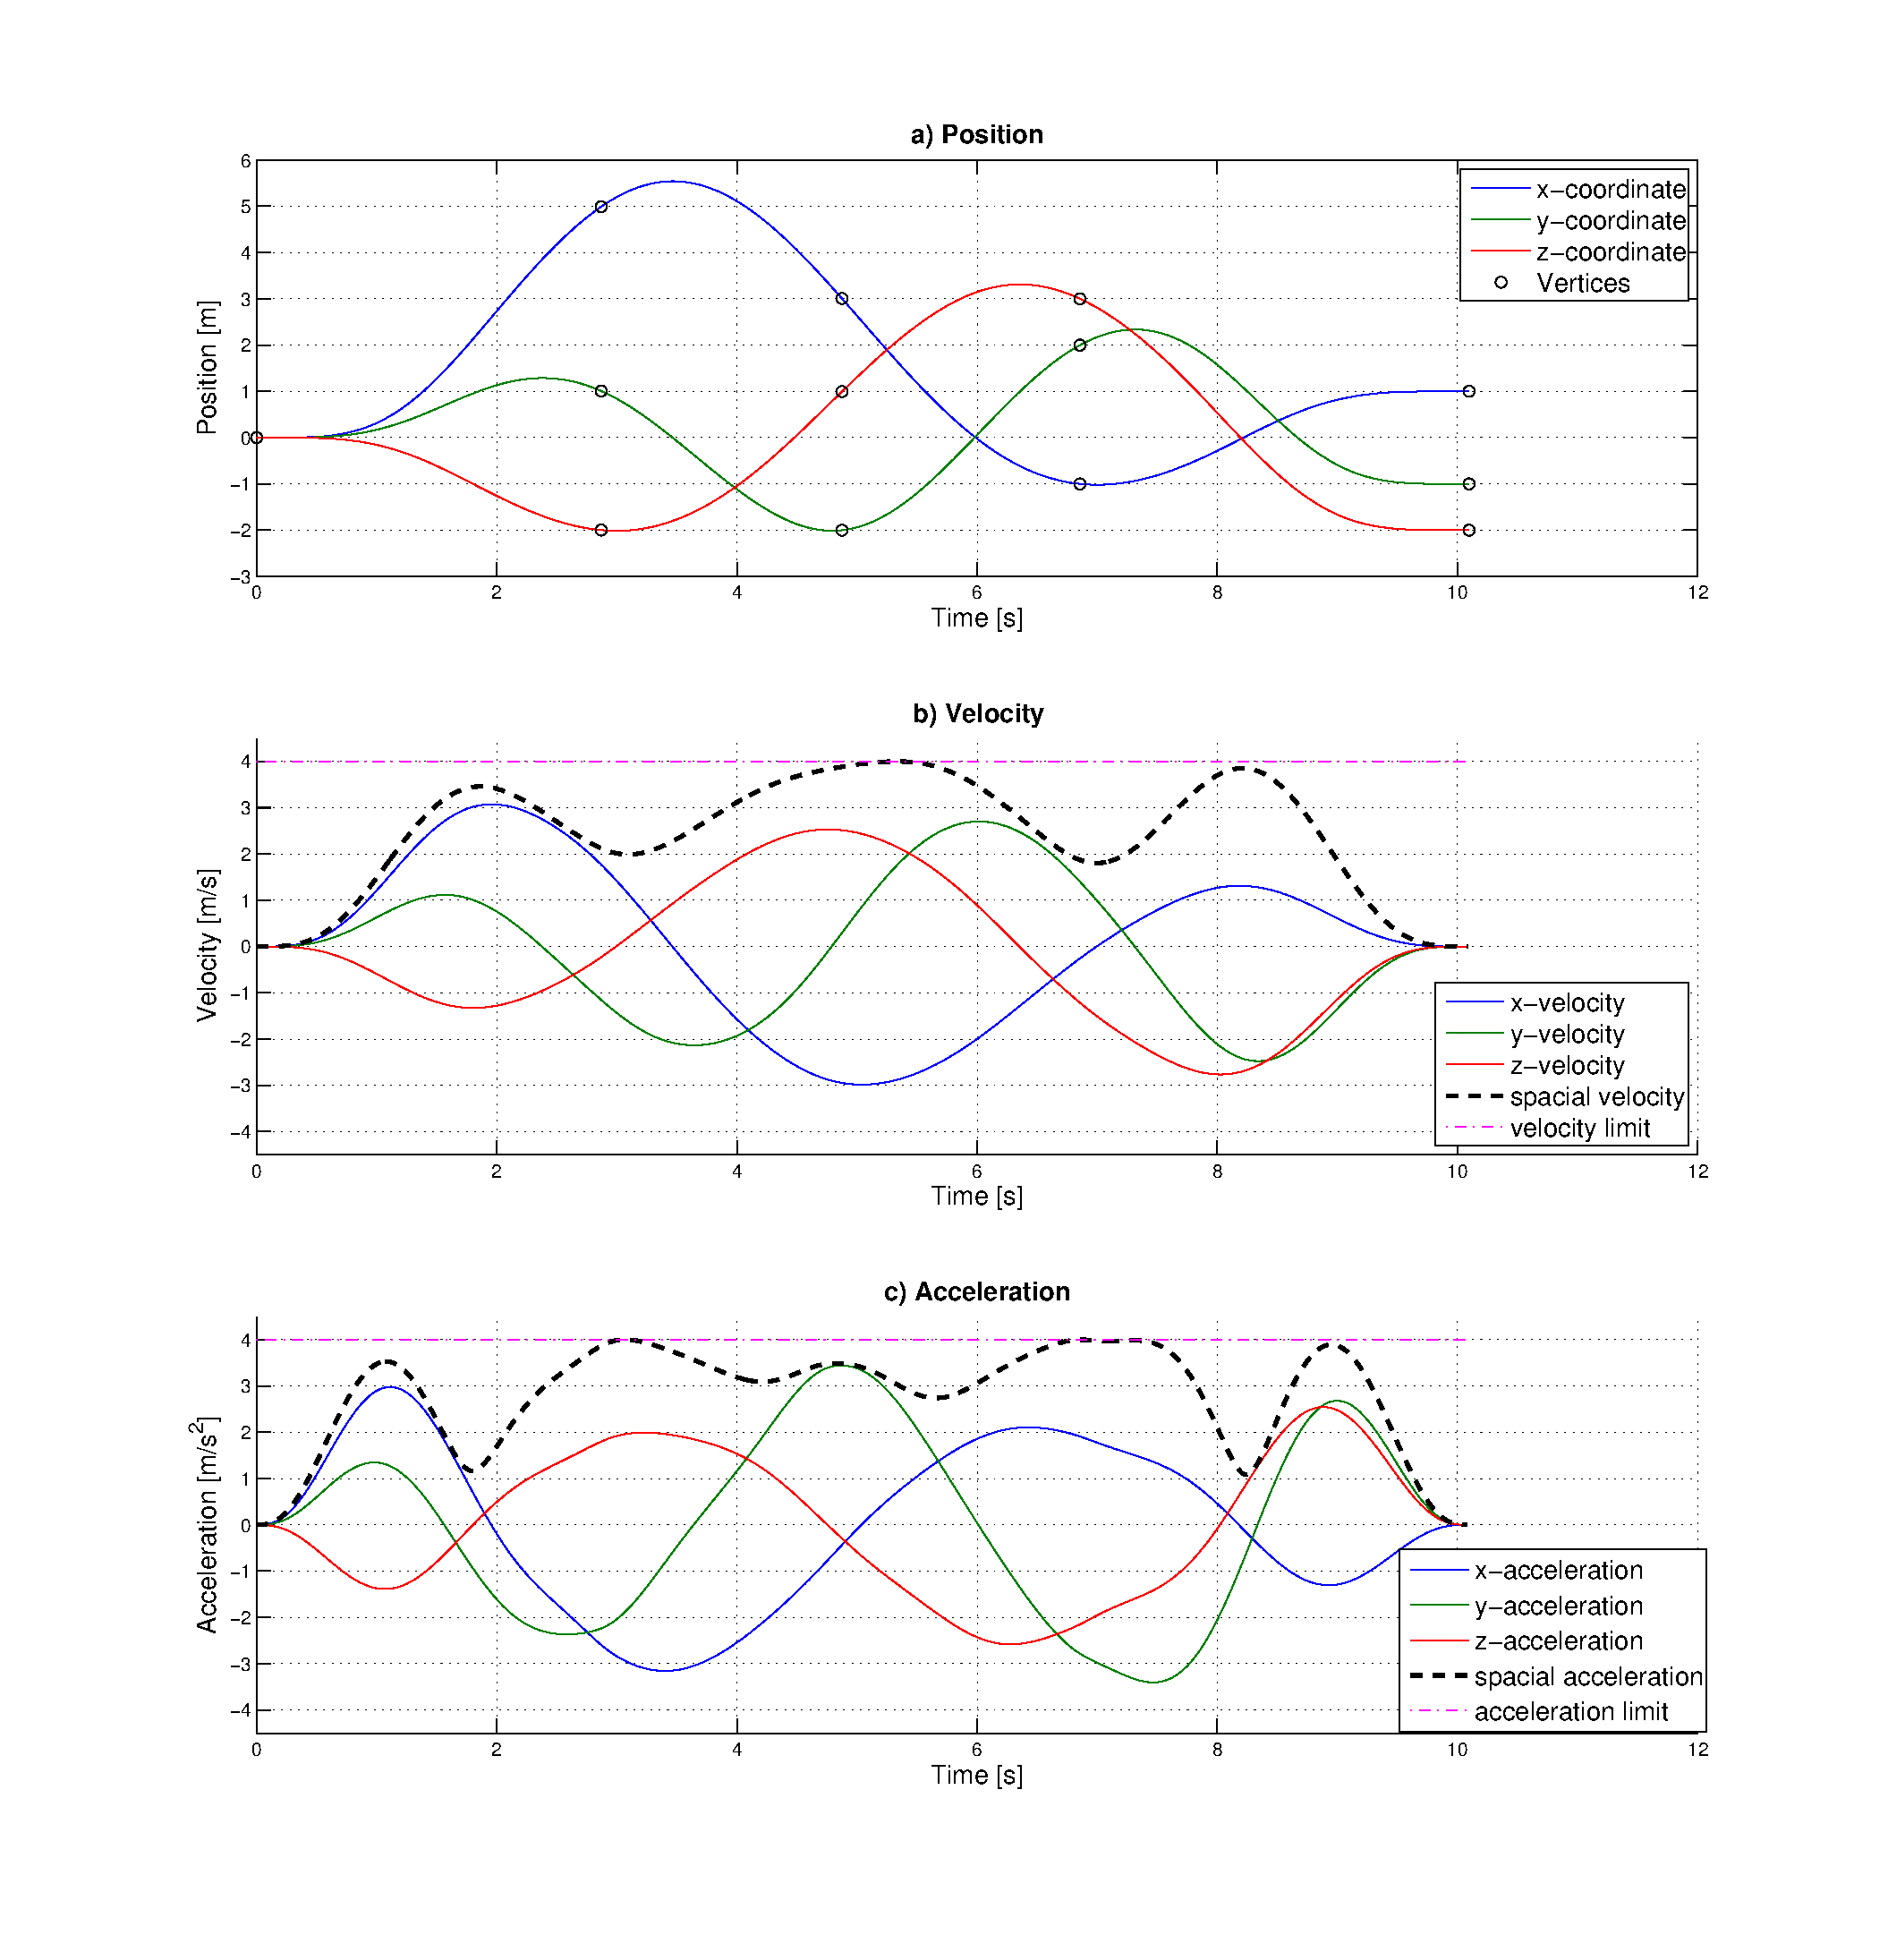
\includegraphics[trim = 35mm 30mm 30mm 15mm,clip,width=1\textwidth]{pics/4SegOpti10s01k2000.eps}
   \caption{Optimized solution of a trajectory with 4 segments: A dashed graph represents the velocity respectively the acceleration in the three-dimensional space. Weighting factor $k_T$ was set to 2000.}
   \label{pic:optimizedSolution4optik2000} 
\end{figure}

In contrast to the aggressive trajectory depicted in figure \ref{pic:optimizedSolution2k2000}, the acceleration limit has a impact on the optimized curvy trajectory in figure \ref{pic:optimizedSolution4optik2000}. As can be seen in plot c) the spacial acceleration touches the acceleration limit repeatedly and even stays at exact $4 \frac{m}{s^2}$ for some time. 

\section{Pathway of the Trajectory}\label{sec:pathway}

The pathway of a snap minimized trajectory is mainly determined by the ratio of the segment times and not by the segment times themselves or by the total trajectory time. As mention in section \ref{sec:drawbackInitial}, the segment times from the initial solution do not incorporate the circumstances from one segment to an other. Hence, it is likely to find a better trajectory with the same total time but a different ratio between the segment time. The process of optimizing the ratio of the segment times is implicitly performed during the process of nonlinear optimization. In other words, the nonlinear optimization not only changes the total trajectory time according to the weighting factor $k_T$ but also optimizes the ratio of the segment times. \newline
Such a change in the pathway is distinguishable between the initial trajectory in figure \ref{pic:optimizedSolution4init} a) and the optimized trajectory in figure \ref{pic:optimizedSolution4optik2000} a). The easiest notable difference is the peak of the $x$ graph with a peak value of 6.95 in the initial trajectory and a peak value of 5.58 in the optimized trajectory. Nevertheless, the changes in the pathway are more presentable in a 3D plot. 


\begin{figure}[H]
   \centering
   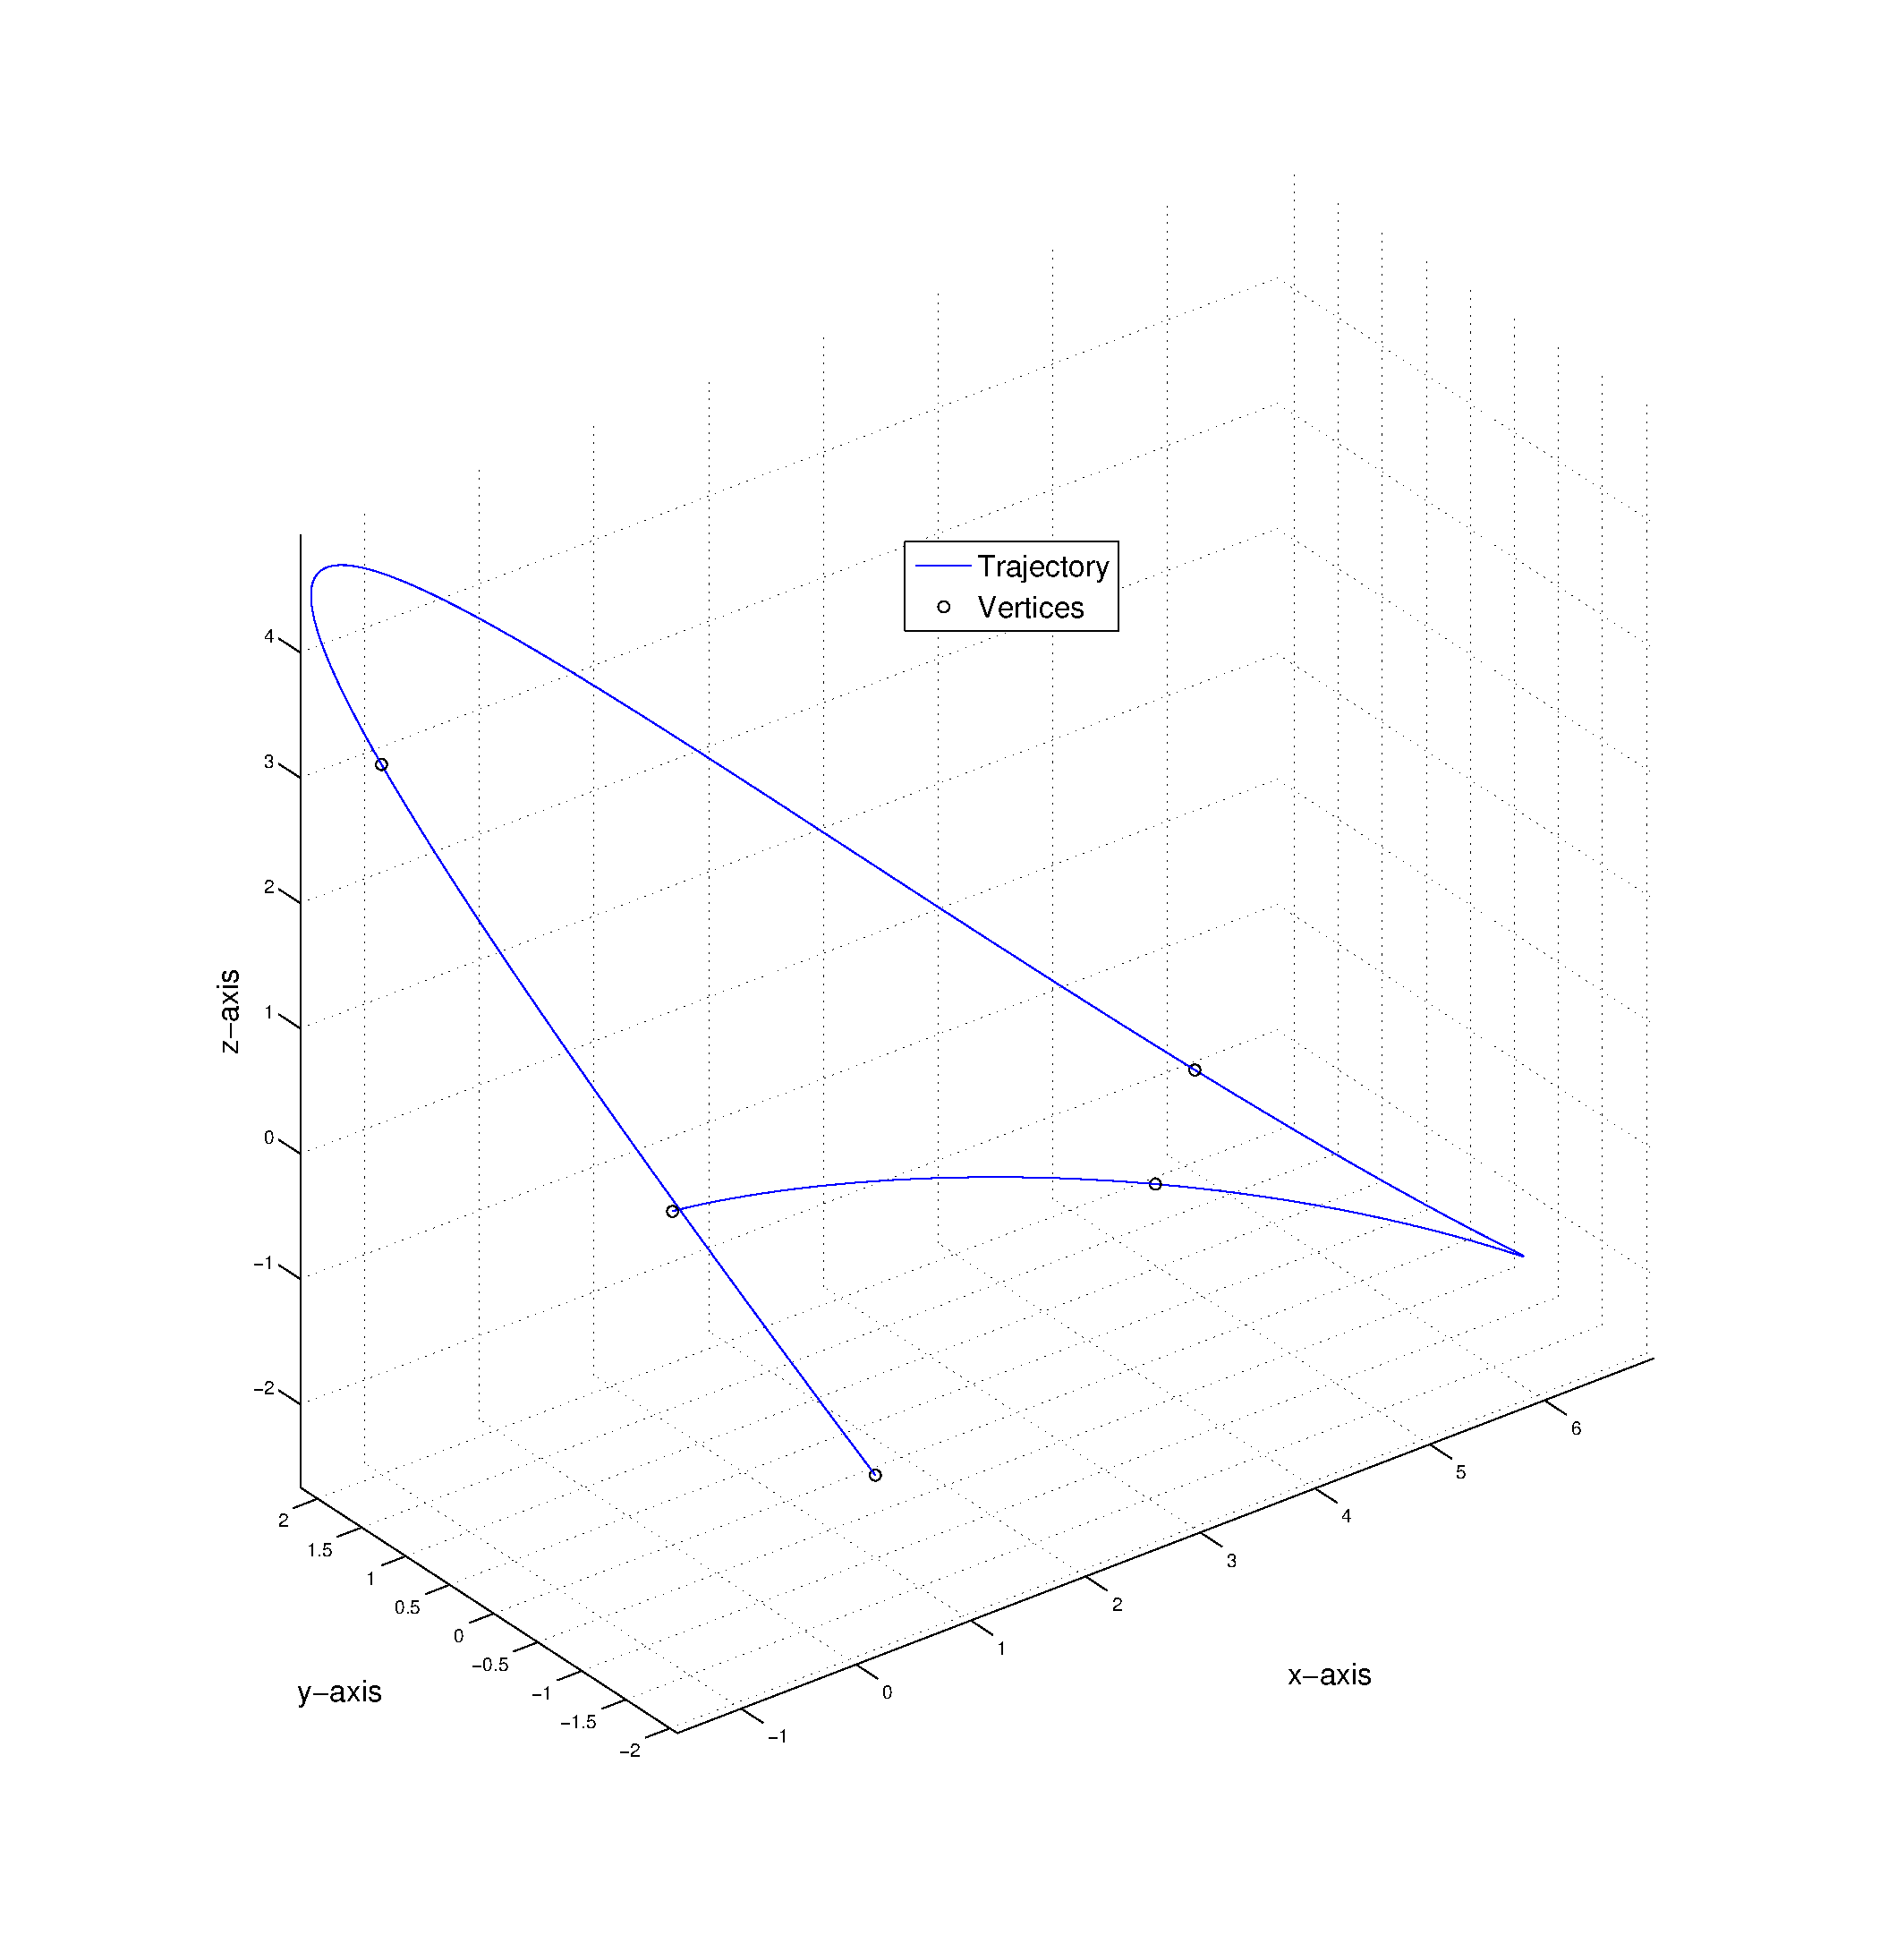
\includegraphics[trim = 36mm 30mm 33mm 30mm,clip,width=1\textwidth]{pics/4SegInitSpace.eps}
   \caption{3D plot of the initial trajectory with 4 segments.The start vertex is located at (0/0/0) and the trajectory proceeds clockwisely.}
   \label{pic:initiSpace} 
\end{figure}


Figure \ref{pic:initiSpace} depicts the initial trajectory (from figure \ref{pic:optimizedSolution4init}) in 3D space. Again, the vertices are marked as circles but now the times is no longer explicit readable. The start vertex is located at (0/0/0) and the trajectory proceeds clockwisely. The second segment (lower right corner) of the initial trajectory in figure \ref{pic:initiSpace} looks very sharp. Such sharp corners, accrued by the suboptimal segment time ratio, are undesirable if the UAV should fly a trajectory dynamically. \newline

The optimization of the ratio of the segment times, which is implicitly performed during the nonlinear optimization, modifies the pathway of the trajectory which gets smoother, i.e. no sharp corner exist in the optimized trajectory.\newline 
Figure \ref{pic:optiSpace} depicts the optimized trajectory (from figure \ref{pic:optimizedSolution4optik2000}) in 3D space. Especially the second segment of the optimized trajectory is now more suitable for a dynamic flight. But also the pathway in the region of the 4. vertex (in the upper left corner) is enhanced. The initial trajectory mad a detour before passing the 4 Vertex. This detour, accrued by the suboptimal segment time ratio, is vanished in the optimized trajectory.



\begin{figure}[H]
   \centering
   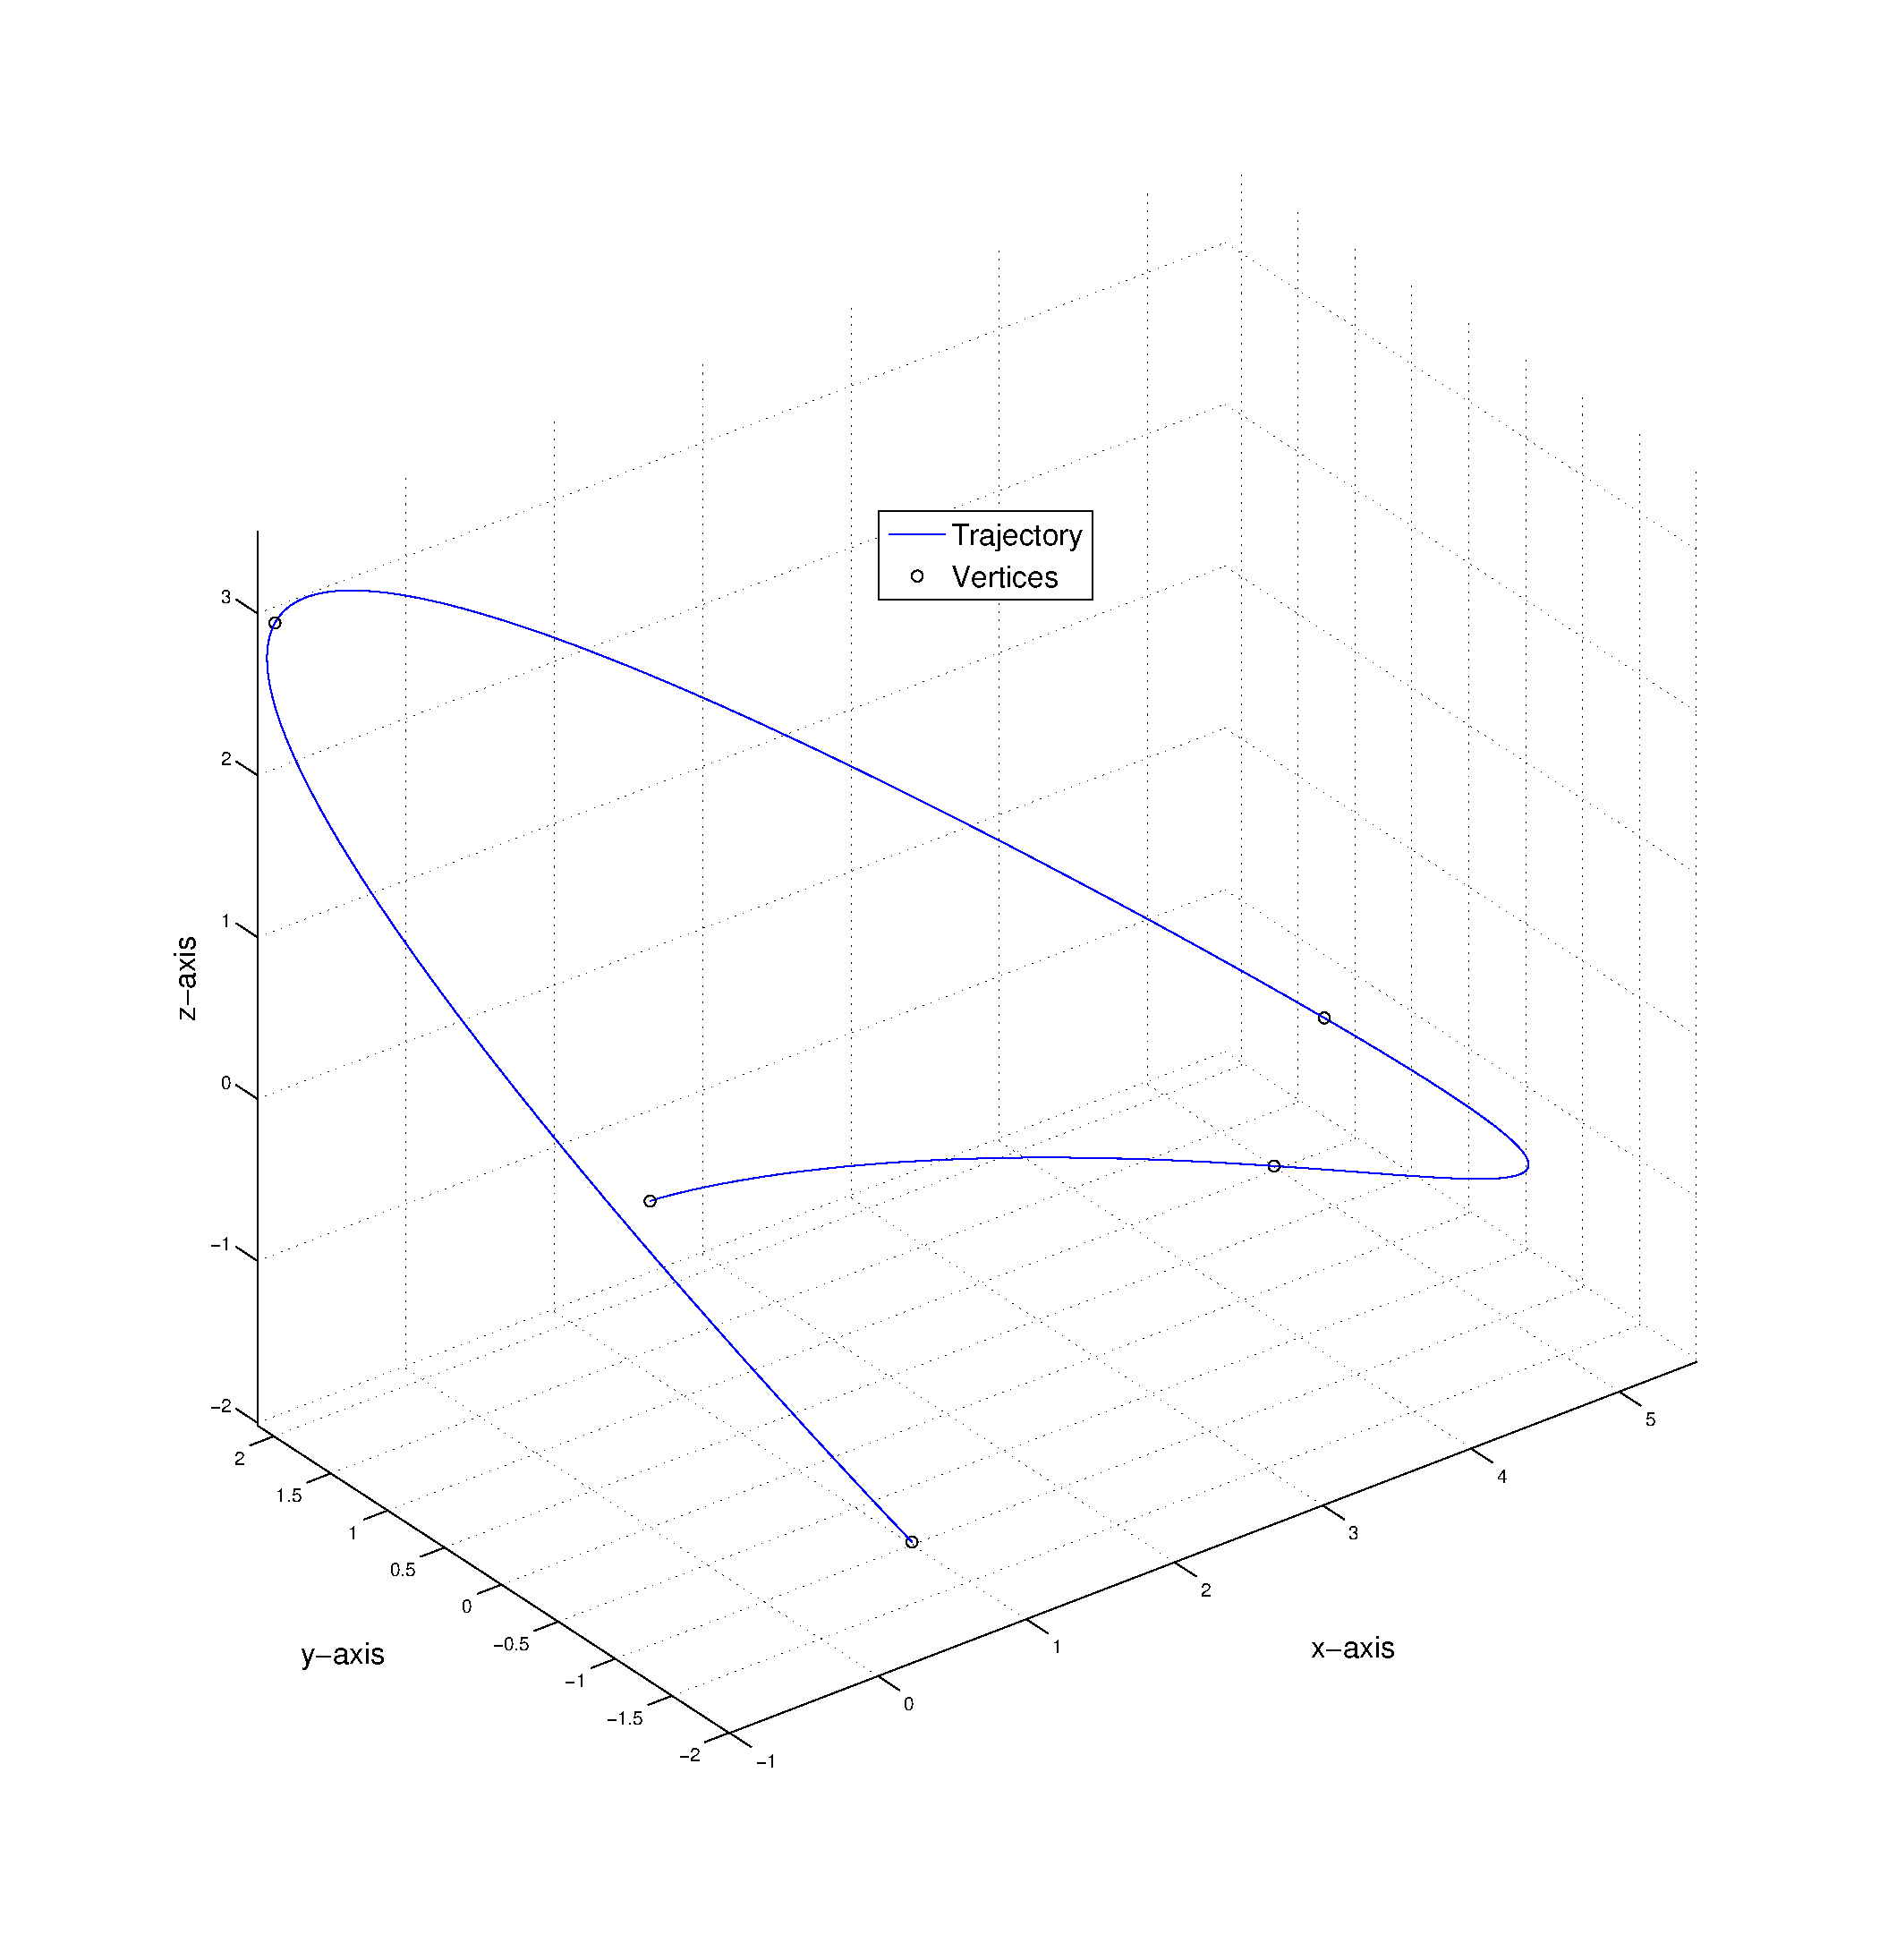
\includegraphics[trim = 36mm 30mm 33mm 30mm,clip,width=1\textwidth]{pics/4SegOptiSpace.eps}
   \caption{3D plot of the optimized trajectory with 4 segments.The start vertex is located at (0/0/0) and the trajectory proceeds clockwisely.}
    \label{pic:optiSpace} 
\end{figure}
\newpage


\section{NLopt}\label{sec:NLopt}

For all the nonlinear optimizations which were performed in the previous sections, NLopt, a open-source library for nonlinear optimization, was applied. The optimization algorithm tries to minimize the cost function every iteration and needs some kind of termination condition in order to know when to stop.\newline
The termination condition of the optimization can be specified by the optimization variables as well as by the total cost. Generally, the termination conditions are formulated relative to the current value(s). For instance, if the relative termination condition for the total cost $J_{rel}$ is set to $0.01$ the optimization ends if the total cost changes less than one percent during an iteration. The relative termination condition for the optimization variables $x_{rel}$ is only fulfilled if all of the optimization variables change less than the threshold in an iteration.
Additionally, an absolute termination condition $x_{abs}$ can be applied to the optimization variables. This termination condition is only needed if one or several optimization variables are close to zero and the relative criteria therefore don't work properly. \newline 
Two additional options are the limitation of the number of optimization iterations and the limitation of the duration of the optimization. All of these termination condition can be set simultaneously and the first condition which is fulfilled stops the optimization.
During the optimization the constraints on velocity and acceleration are checked every iteration. \newline










%Once the segment times are calculated, the initial snap minimized solution can be computed according to equation \ref{equ:dpstar}. The initial solution for a 3 dimensional problem with 4 segments is depict in figure \ref{pic:initialSolution}. The start of the trajectory is the origin of the Cartesian coordinate system (0/0/0). For both, start and goal state, the velocity, the acceleration, the jerk and the snap are fixed and set to zero. For all the other sampling points (vertices) the derivatives are unspecified. The Cartesian coordinates of the sampling points are chosen manually and are listed in the following table: 
%




%\begin{figure}[h]
%   \centering
%   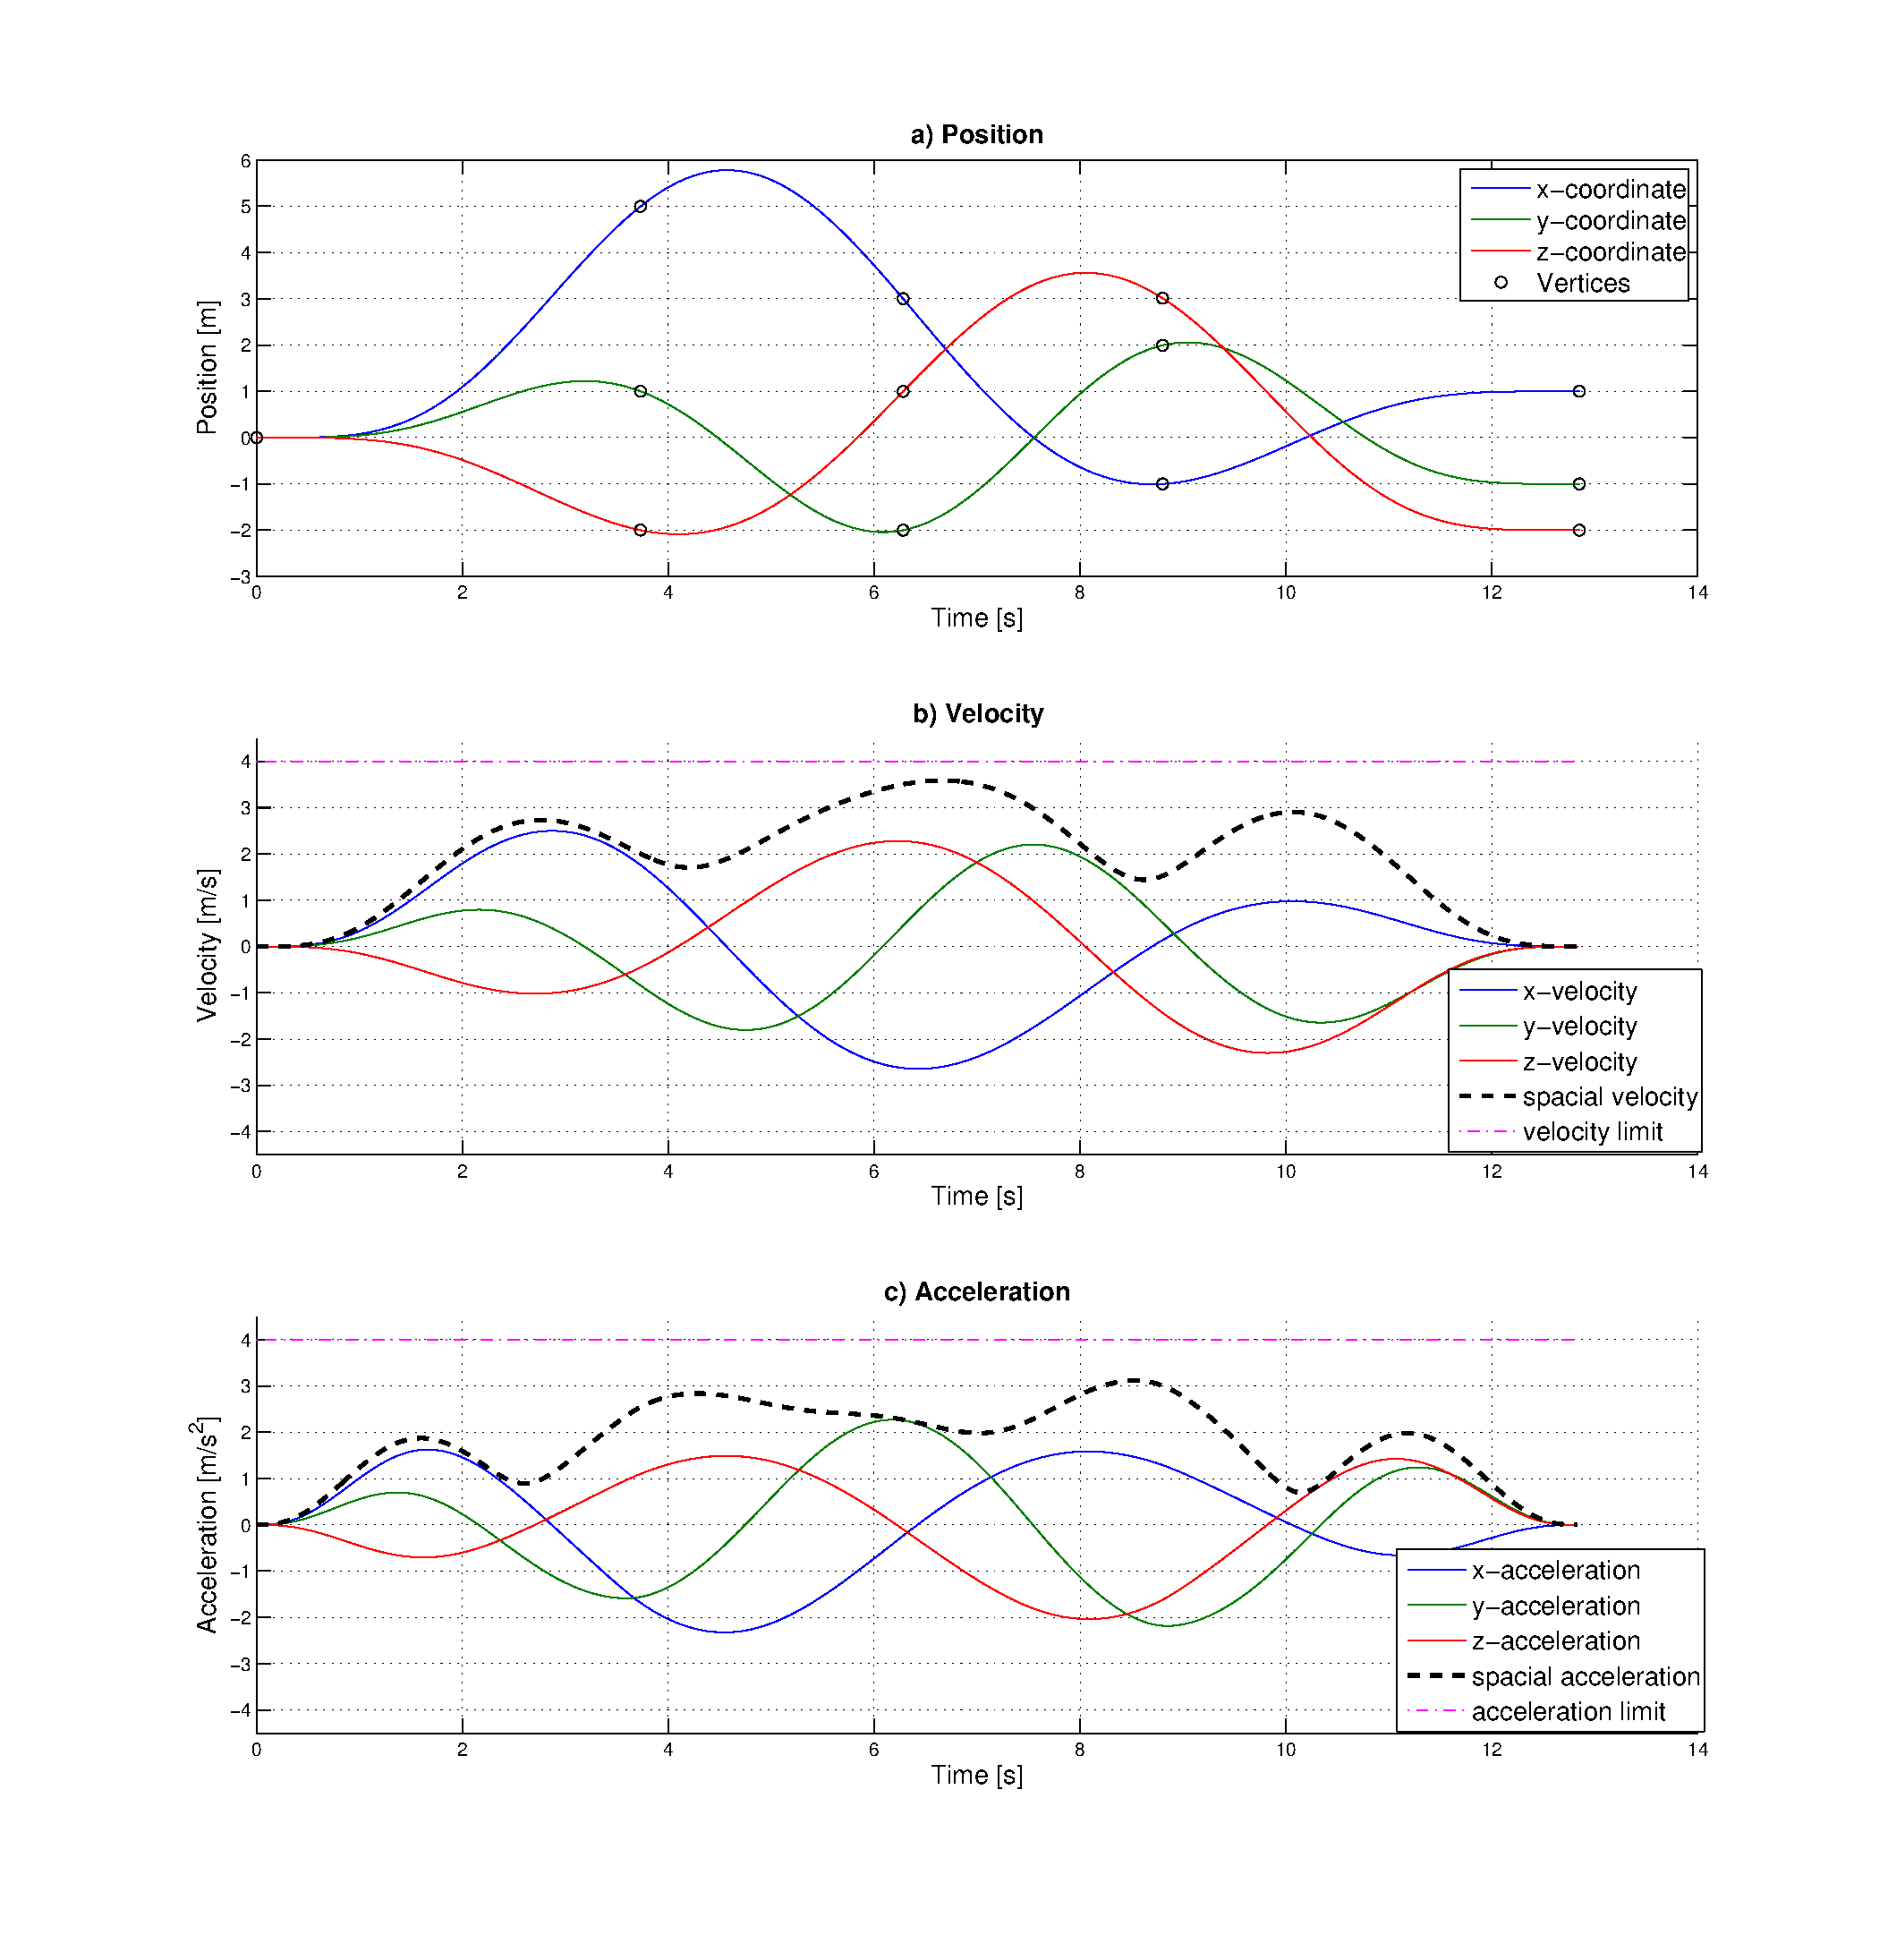
\includegraphics[trim = 35mm 20mm 30mm 35mm,width=1\textwidth]{pics/4SegOpti12s85k100.eps}
%   \caption{...................................................................................... ..... ............. . . . . ...................... ......... .........}
%\end{figure}
%
%
%
%
%





%\texttt{\begin{figure}[h]
%   \centering
%   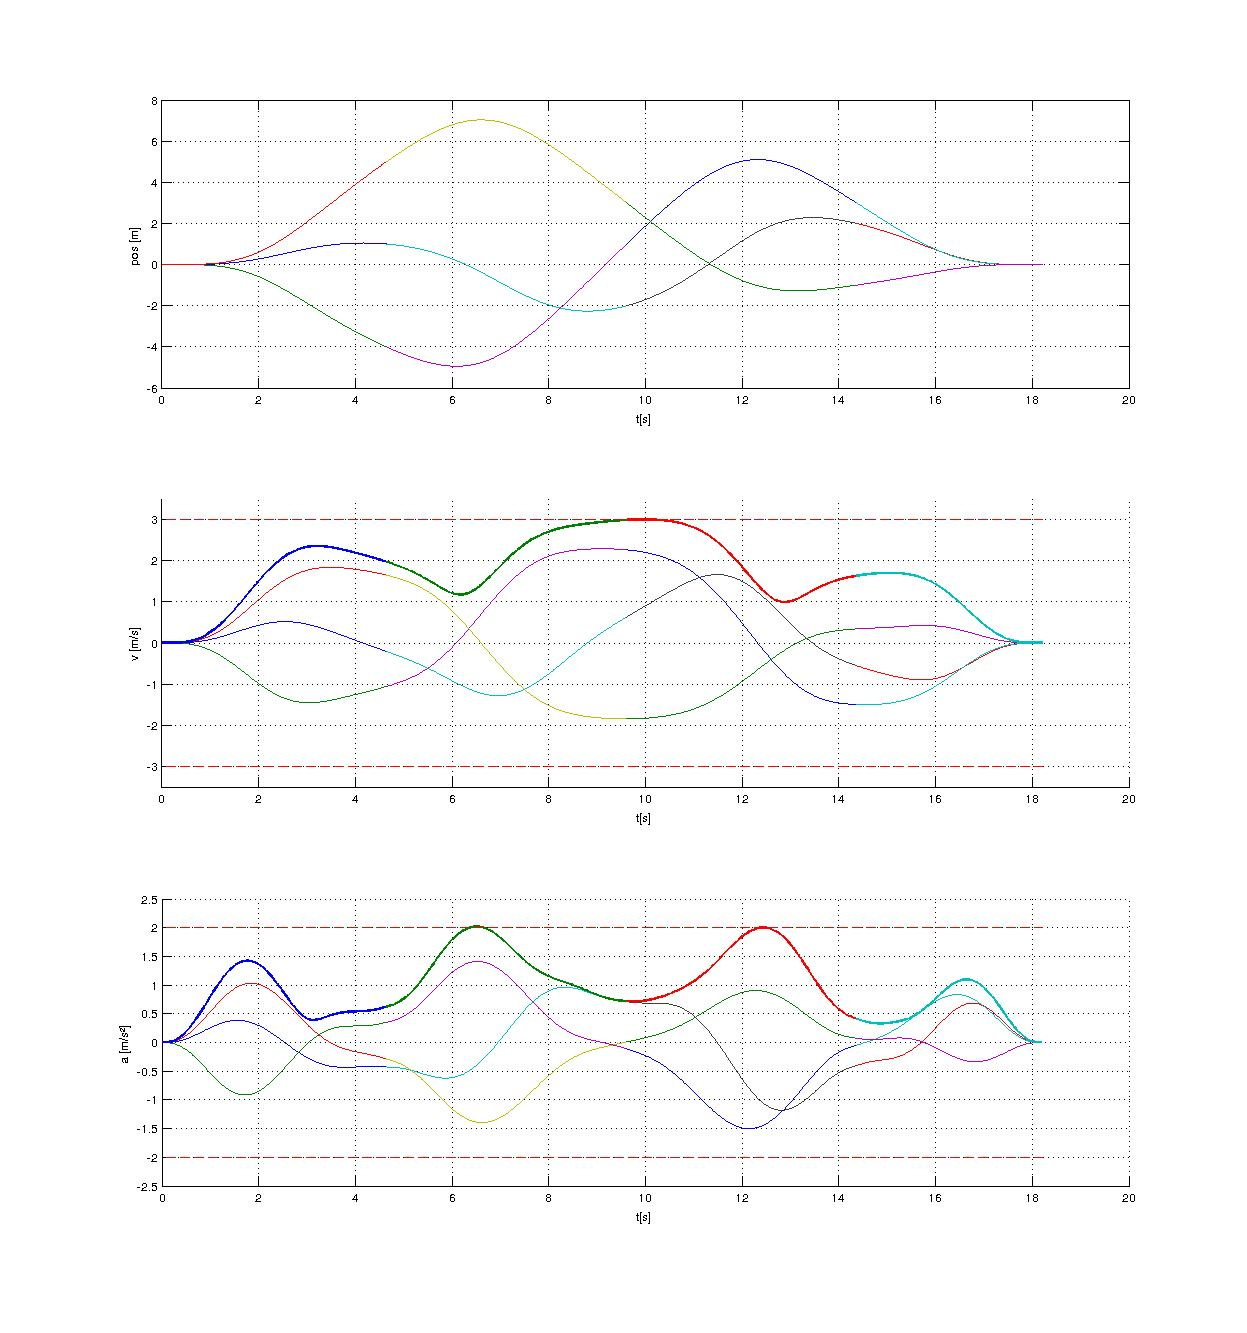
\includegraphics[width=1\textwidth]{pics/optimized.jpg}
%   \caption{Optimized solution of a trajectory with 4 segments: Plot a) shows the position (i.e. the Cartesian coordinates). Plot b) shows the velocity and plot c) the acceleration. A dashed graph represents the velocity respectively the acceleration in the three-dimensional space.}
%   \label{pic:optimizedSolution}
%\end{figure}}





%\begin{figure}[h]
%   \centering
%   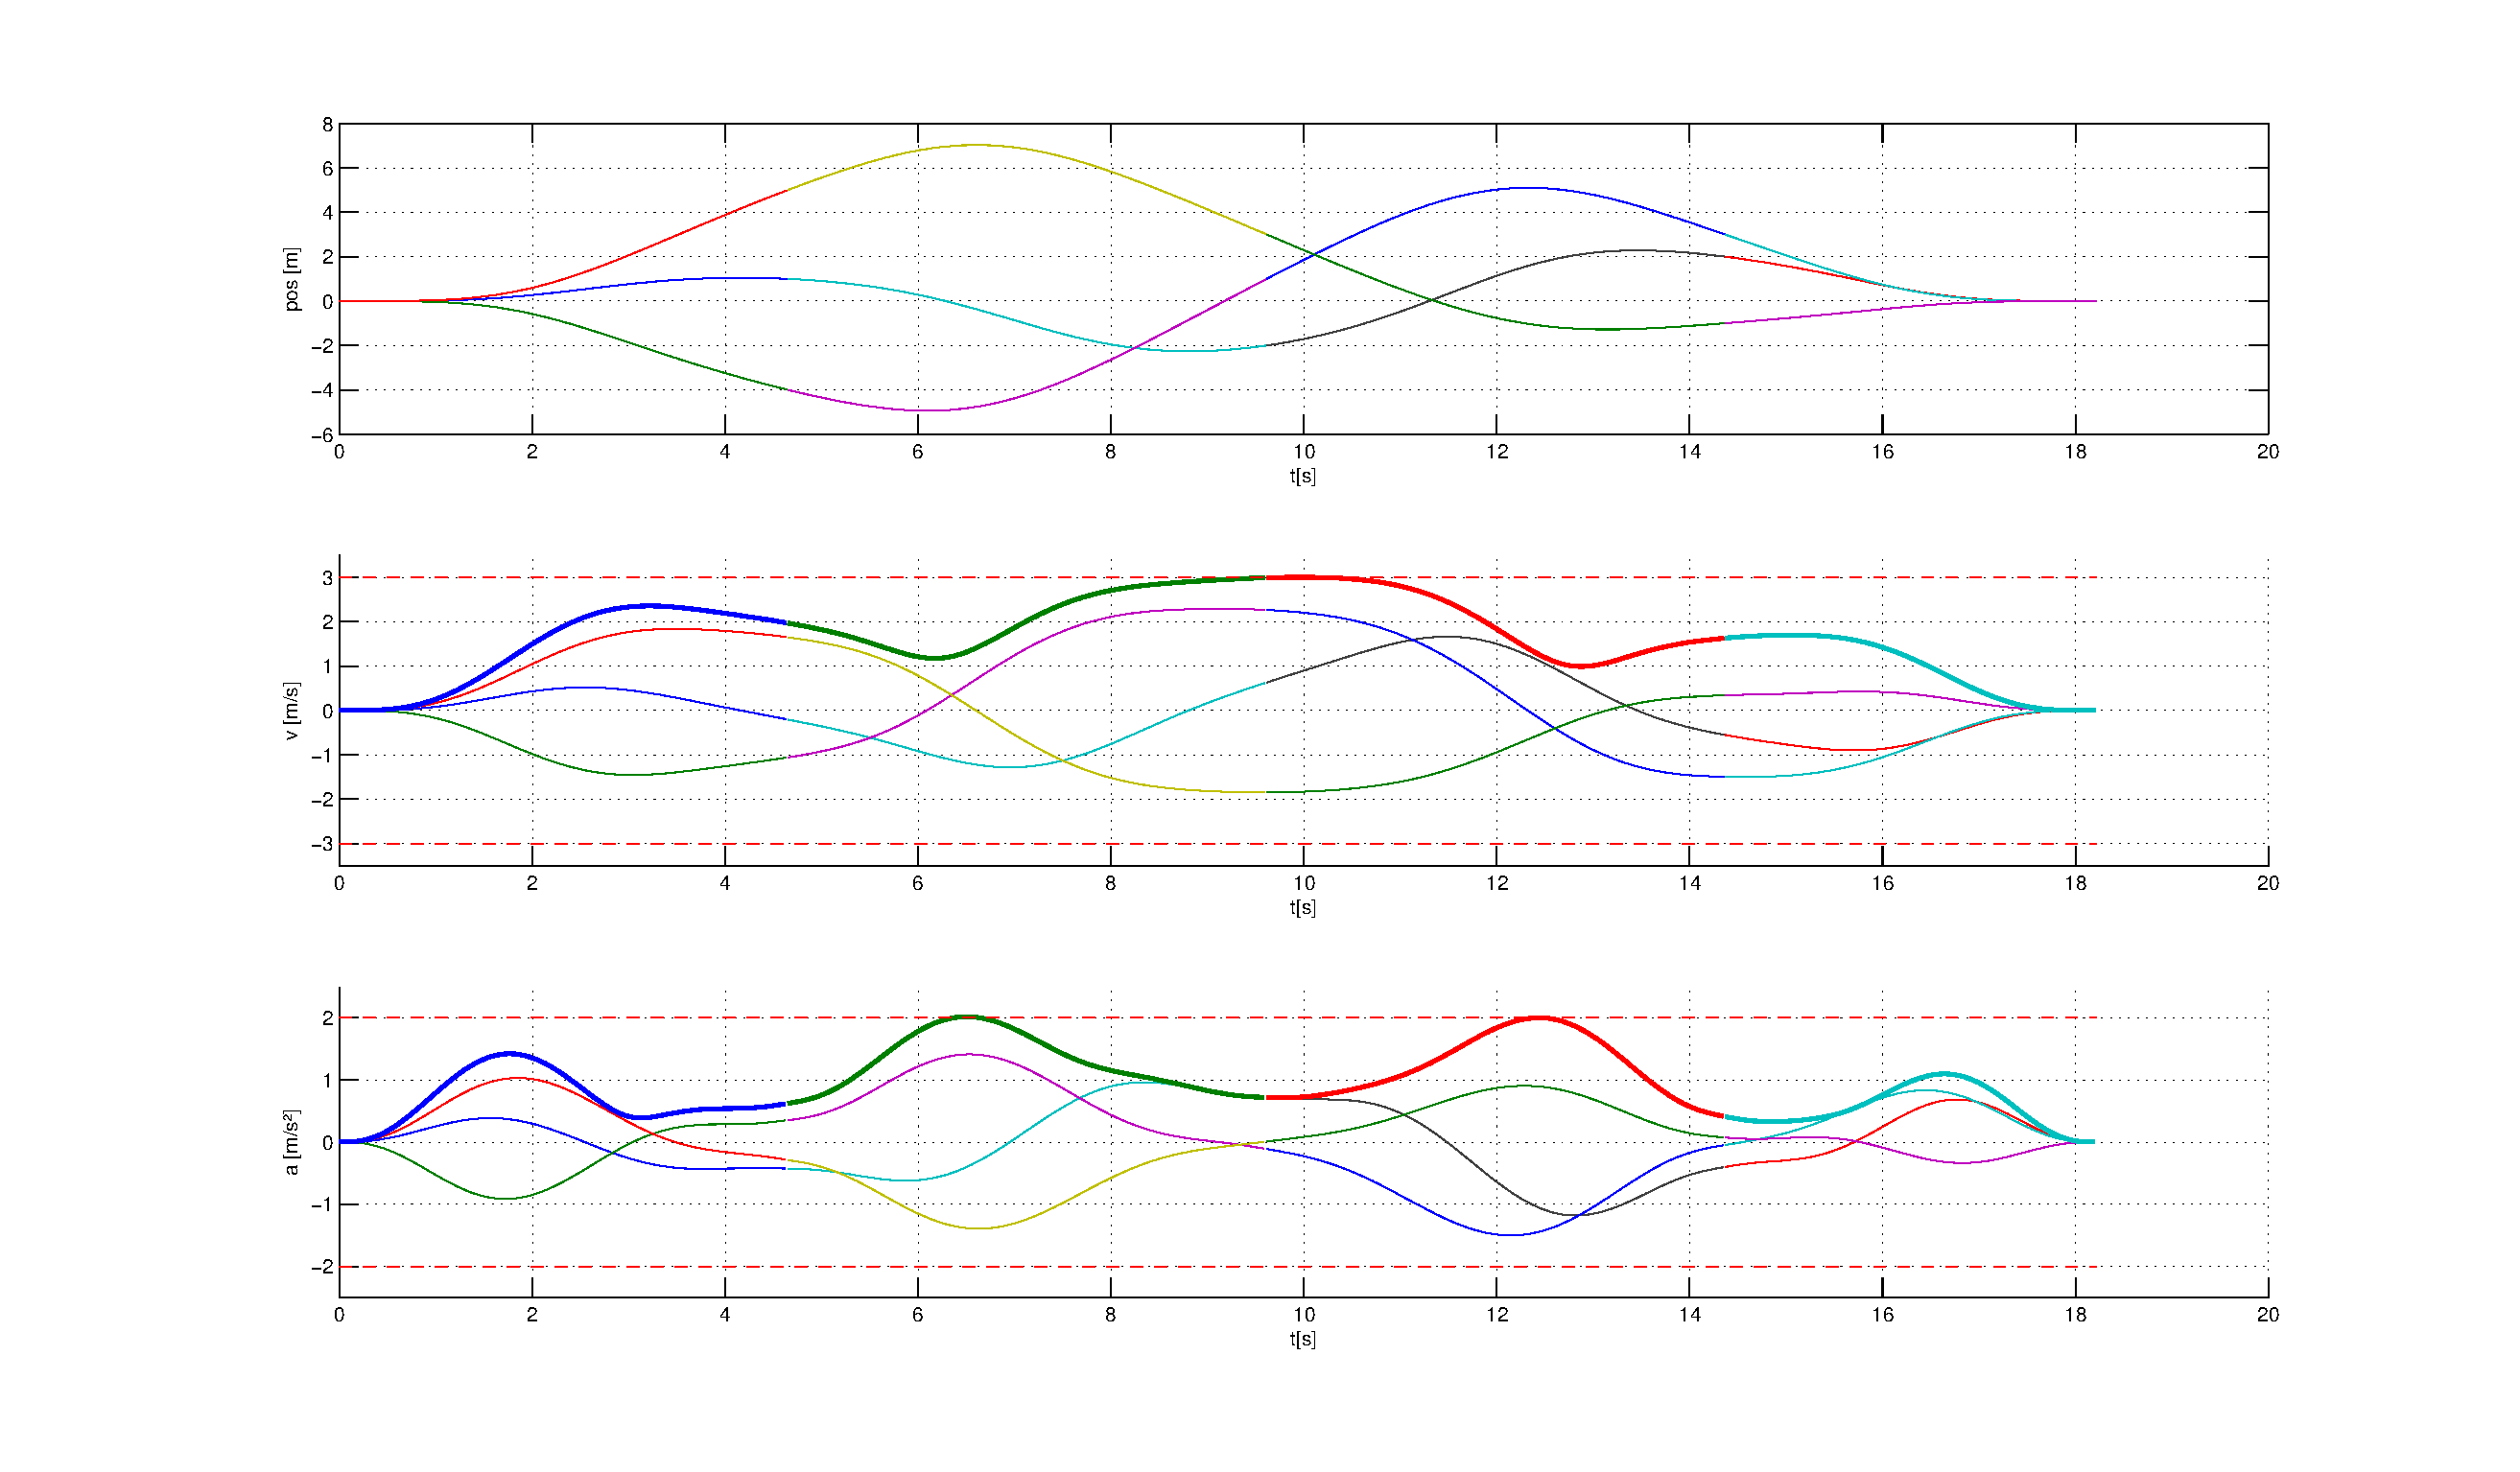
\includegraphics[width=1\textwidth]{pics/optimized.eps}
%   \caption{Ein Bild.}
%\end{figure}
%
%
%\begin{figure}[h]
%   \centering
%   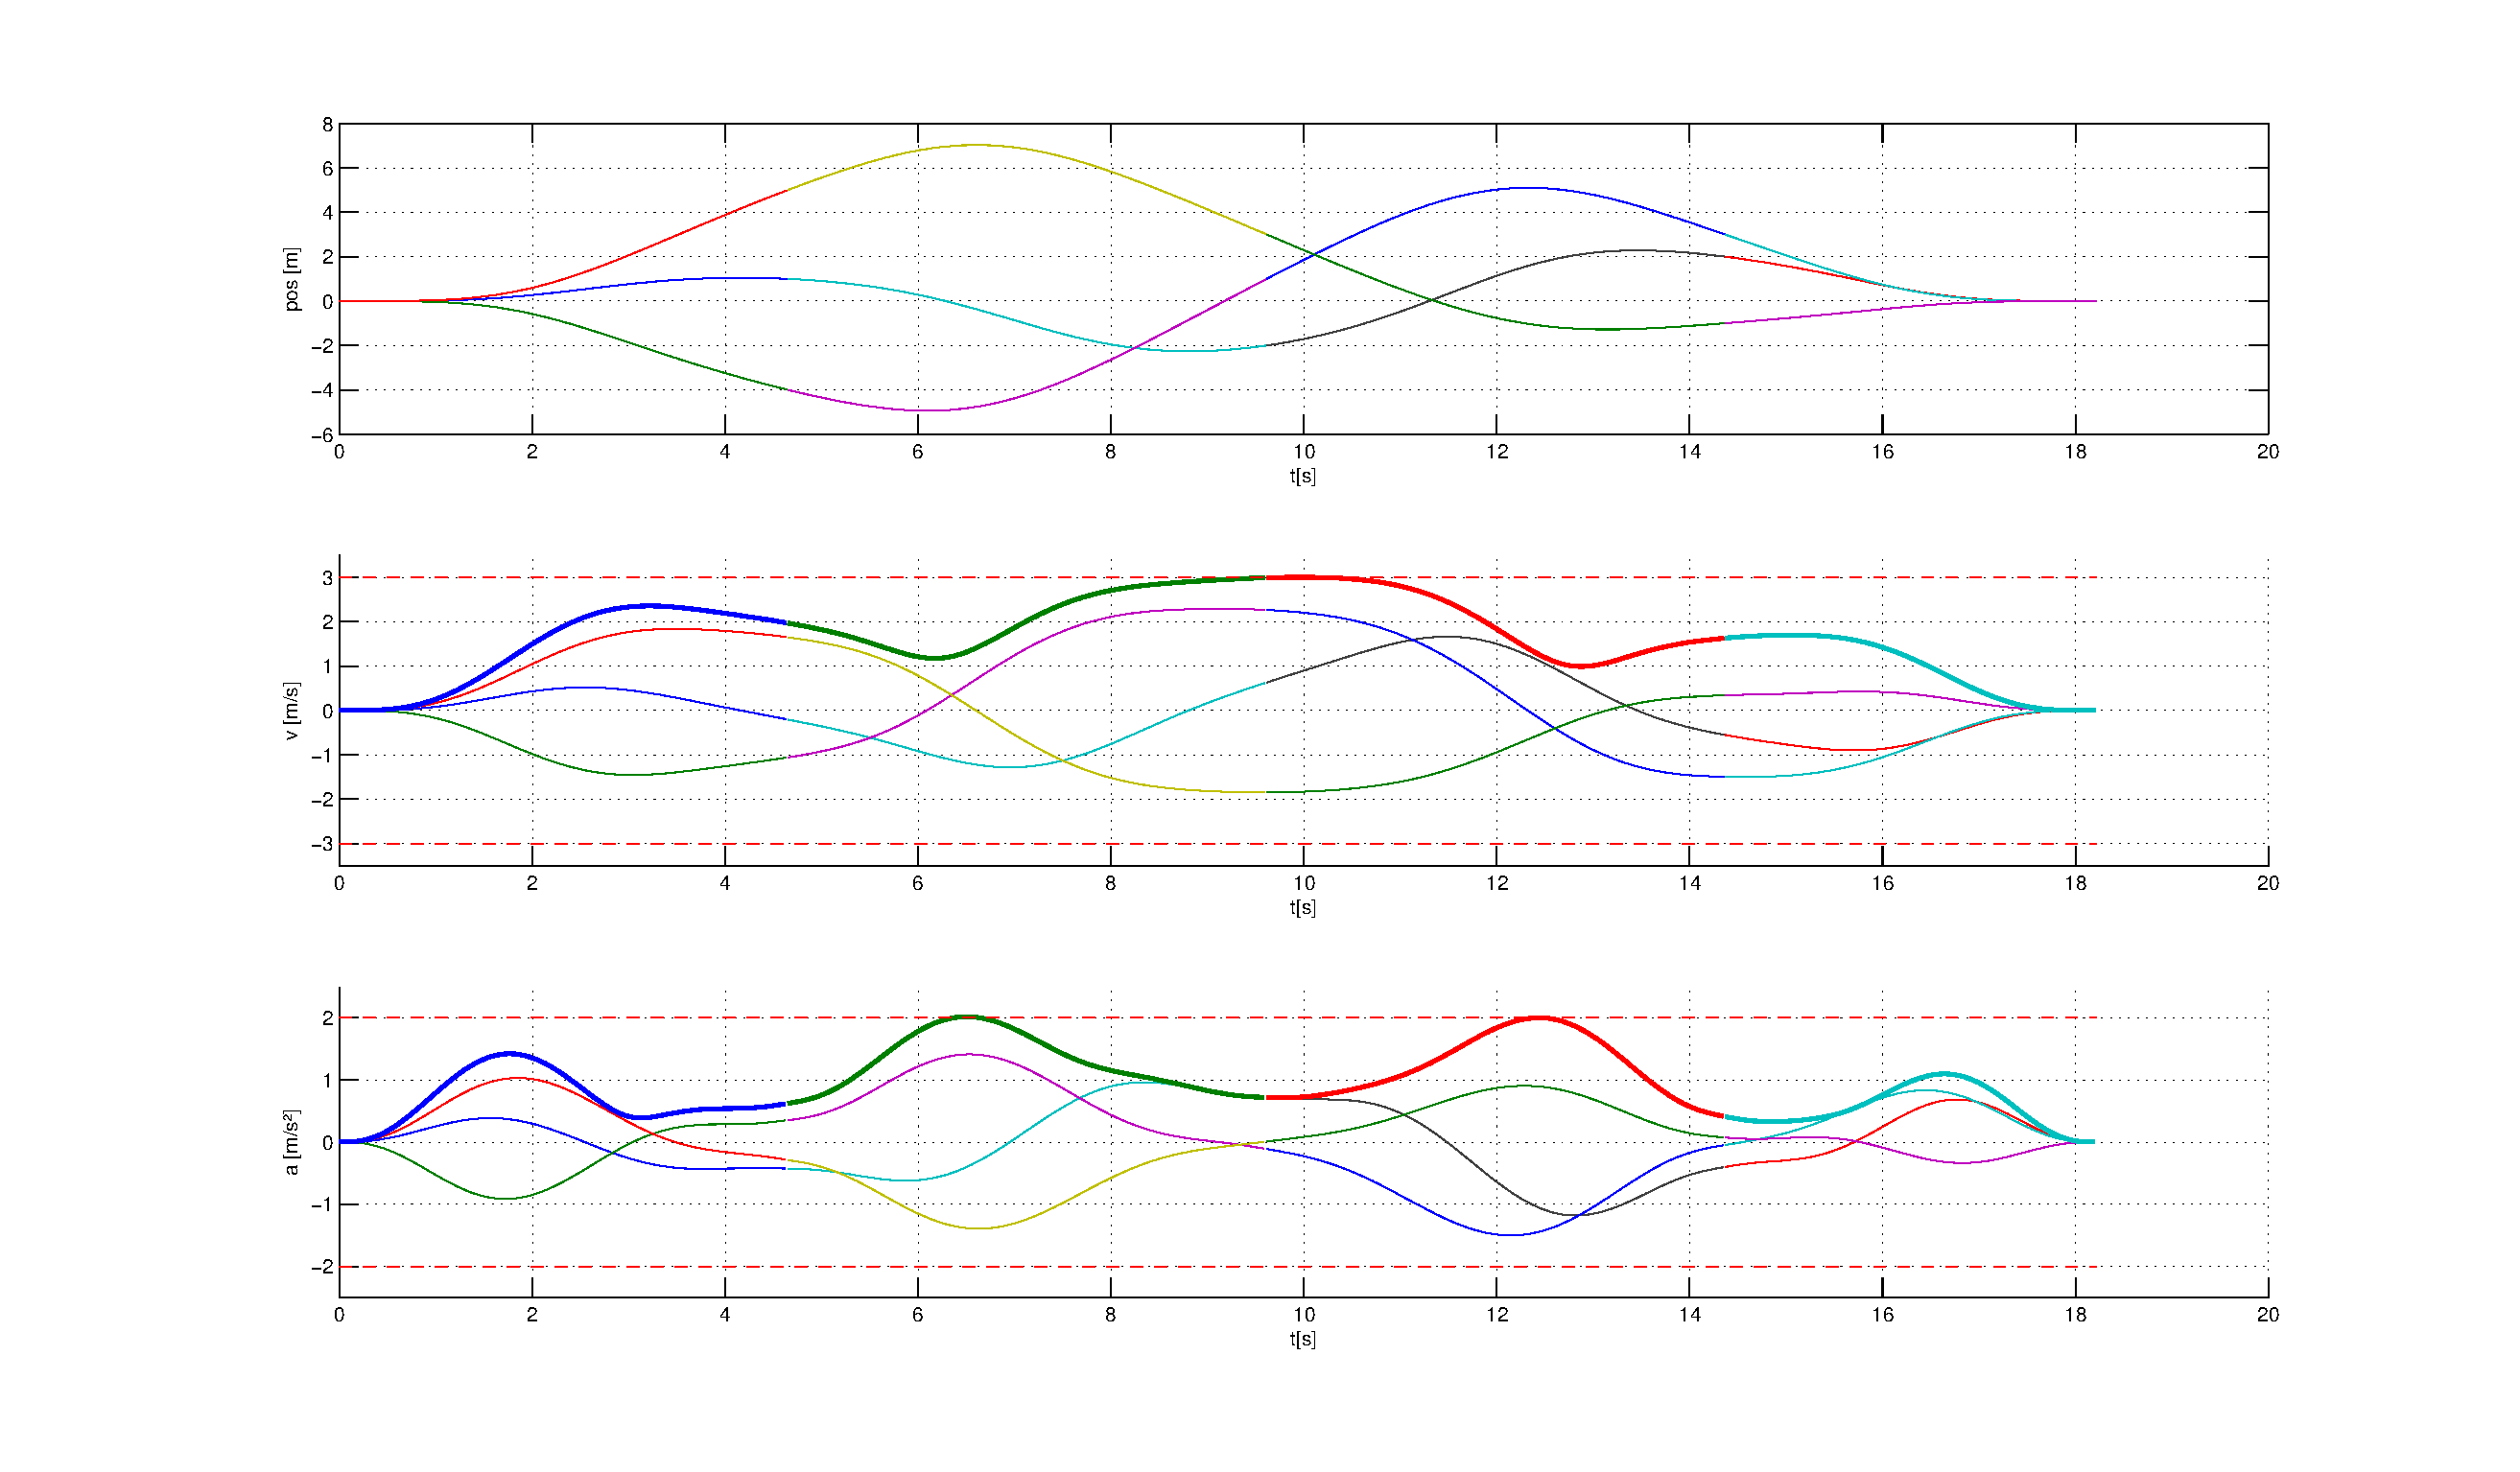
\includegraphics[scale=0.3]{pics/optimized.eps}
%   \caption{Ein Bild.}
%\end{figure}



%\begin{figure}[h]
%   \centering
%   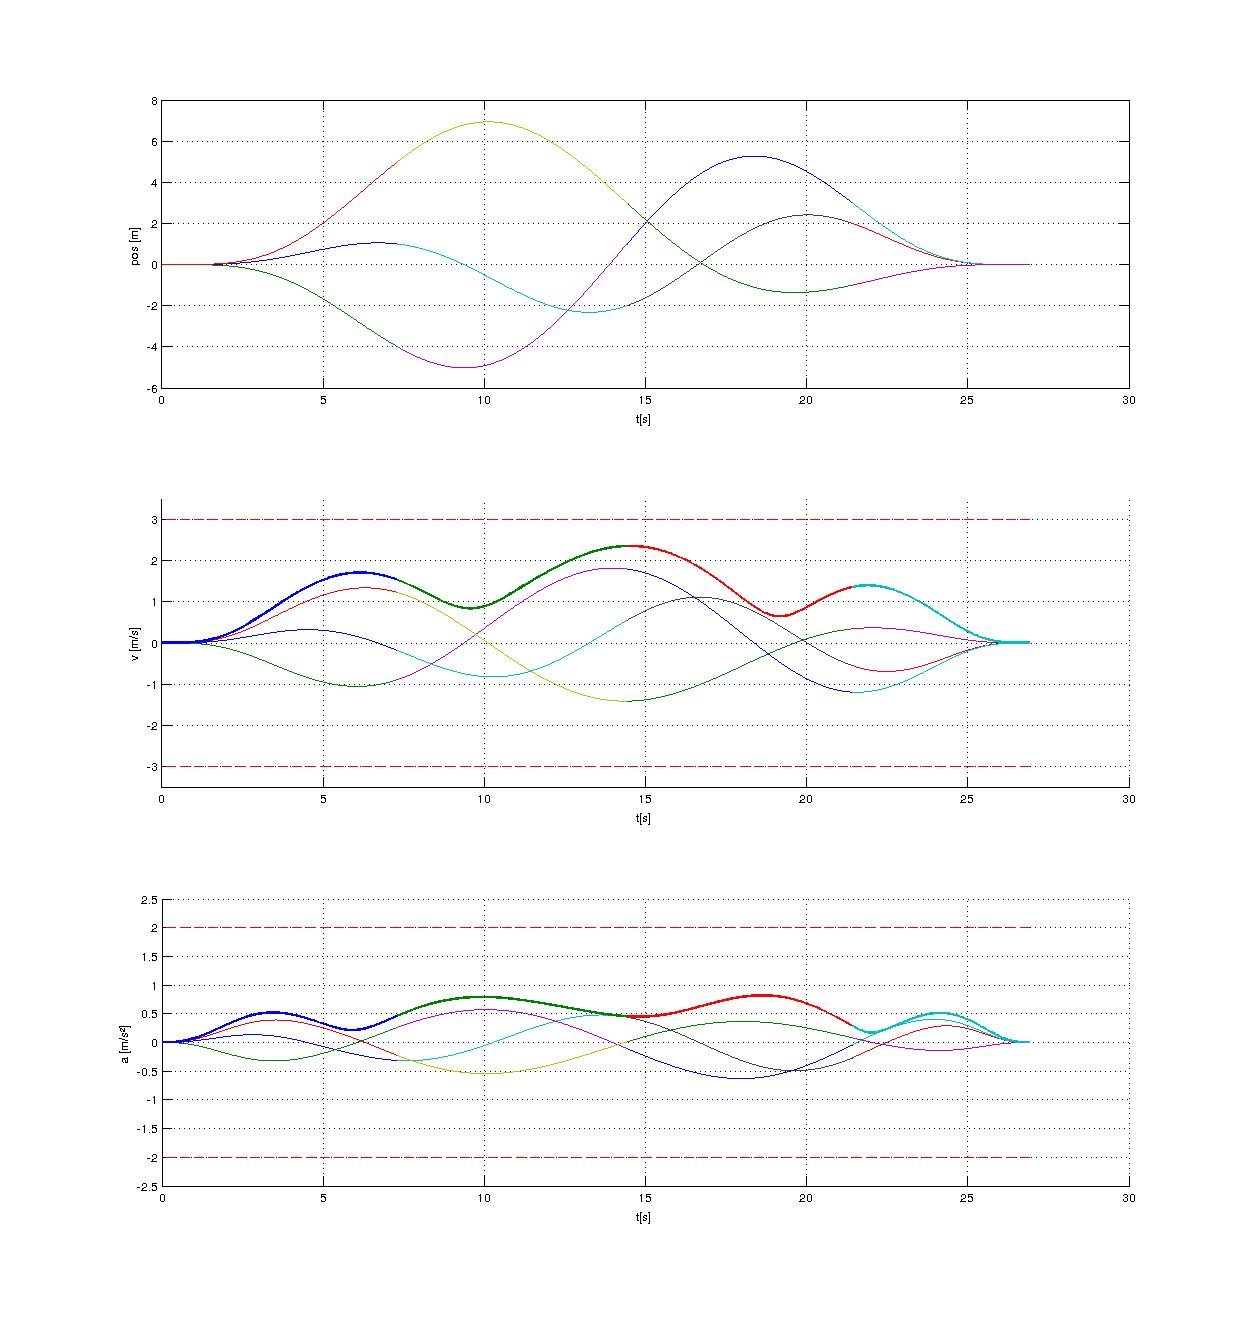
\includegraphics[width=1\textwidth]{pics/initial.eps}
%   \caption{Ein Bild.}
%\end{figure}

%\begin{figure}[h]
%   \centering
%   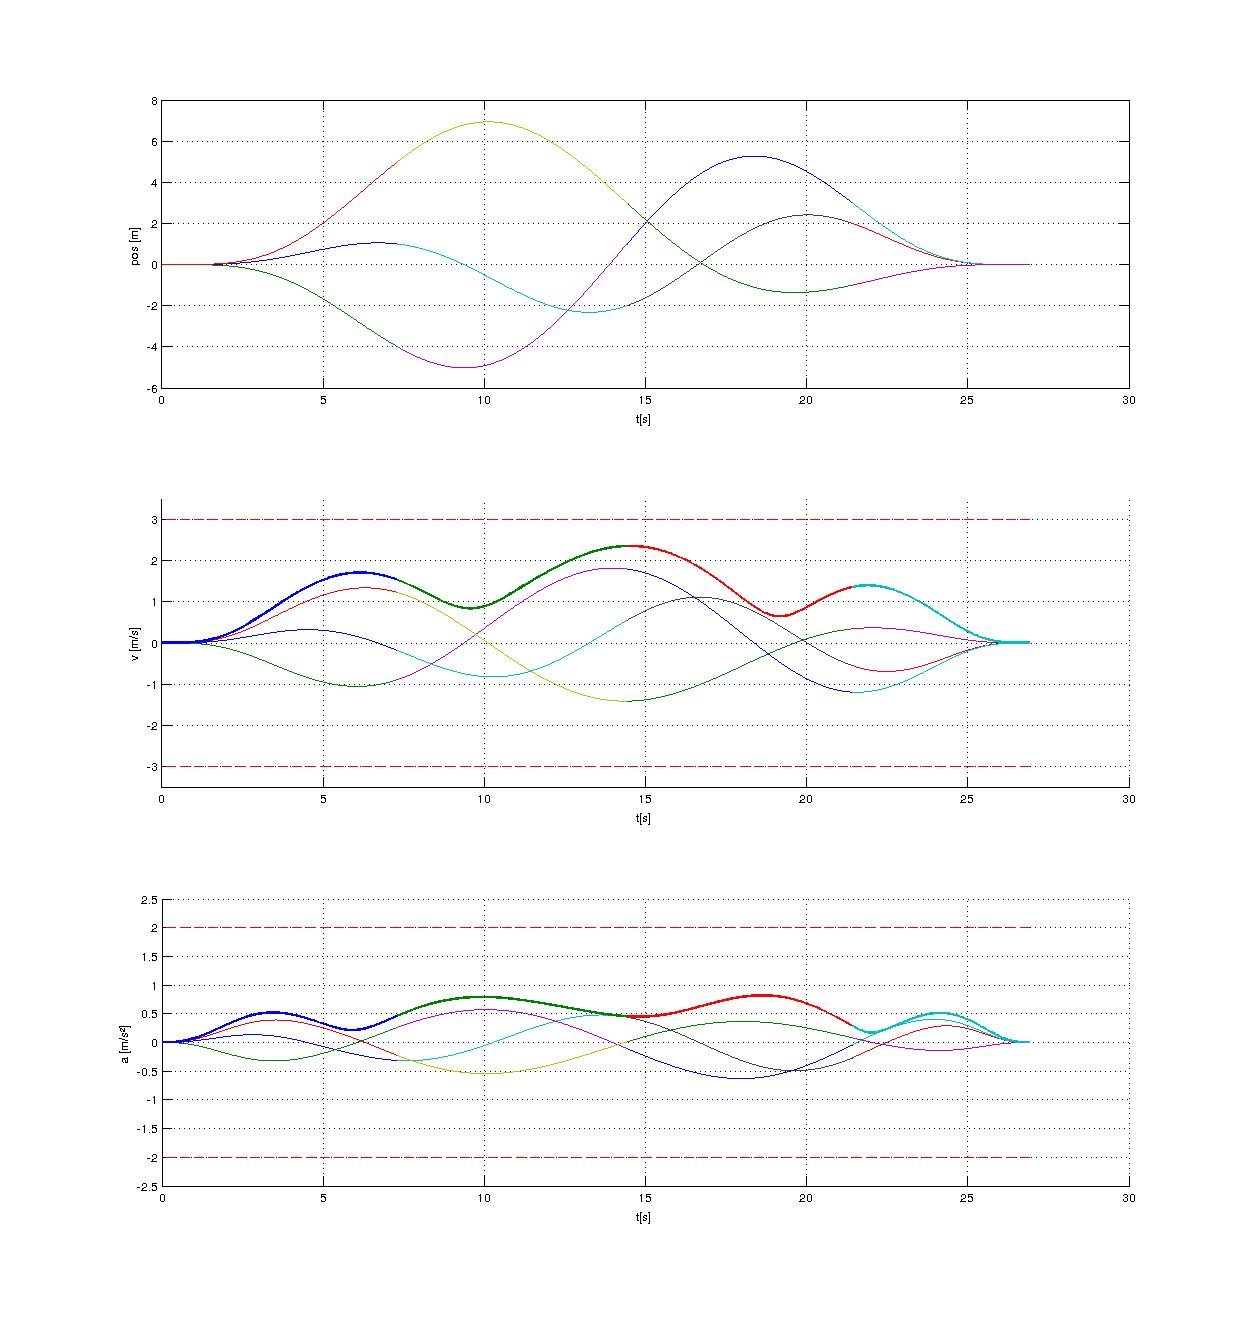
\includegraphics[scale=1]{pics/initial.eps}
%   \caption{Schematic of a rough foot surface.}
%   \label{pics:profile2}
%\end{figure}
























 \cleardoublepage
 \chapter{RRT}\label{chap:RRT}

\section{General}

The goal of this thesis was not only to generate a numerically stable, snap optimized polynomial trajectory but also to explore a densely packed (indoor) environment and plan an aggressive trajectory in between the obstacles. Hence, the Rapidly-Exploring Random Tree (RRT) algorithm is used to find a collision-free straight line solution through densely packed environments. The sampling points oft the RRT (or RRT*) algorithm are then used as the vertices in the polynomial optimization.


\section{RRT Algorithm}\label{sec:RRT}

RRT is a computational efficient algorithm to find a path in a high dimensional space by randomly building a space-filling tree. The sampling points are drawn randomly from the sample space and the tree grows incrementally. 
For each new sample the algorithm attempts to build a collision-free connection to the nearest state in the tree. If a collision-free connection is possible the sample and the connection are added to the tree. \newline

An iteration of the RRT algorithm can be depicted schematically:


\begin{enumerate}
  \item Generate a random sample
  \item Find nearest state in tree
  \item Try to build a collision-free connection to the nearest state
  \item If feasible, add the sampled state and the connection to the tree
\end{enumerate}

\subsection{Goal State}

As mentioned above, the RRT algorithm is based on random samples. Therefore it is very unlikely that a sampled state perfectly matches the desired goal state. \newline

There are two different strategies to enable the RRT algorithm to get to the goal. One strategy is to define not only a goal state but a goal region. Every random sample which is located within the goal region is considered a goal state. As soon as a collision-free connection to a sample in the goal region is established, this trajectory is stored as the best trajectory. At this point the algorithm can be stopped or further iteration can be performed to find a better trajectory to the goal region. Once an other state from the goal region is sampled and the cost of the path to the new state is lower then the cost of the best trajectory, the best trajectory is replaced by the new path. \newline
Another strategy is to steer the RRT algorithm directly to the goal state. In addition to the randomly sampled states the exact goal state is added to the algorithm. The schematic description of an iteration of the RRT algorithm listed in section \ref{sec:RRT} can be modified to represent an iteration with the goal state:

\begin{enumerate}
  \item Insert goal state
  \item Find nearest state in tree
  \item Try to build a collision-free connection to the nearest state
  \item If feasible, add the sampled state and the connection to the tree
\end{enumerate}

In all the cases where a direct collision-free connection between start and goal state is not possible the iteration with the goal state will not succeed in a first attempt. Hence the iterations with the randomly sampled states described in section \ref{sec:RRT} are needed to build the space filling tree.\newline

Figure \ref{pic:smallGamma} depicts the straight line solution of the RRT algorithm with a fixed goal state. The figure is in bird's eye perspective and shows a crossing of different hallways. The blue cells represents the floor and the green cells represents the walls. The map was generated with a stereo camera and was not reworked. Therefore some of the cells of the floor which should be occupied/blue are left free. 

\begin{figure}[H]
   \centering
   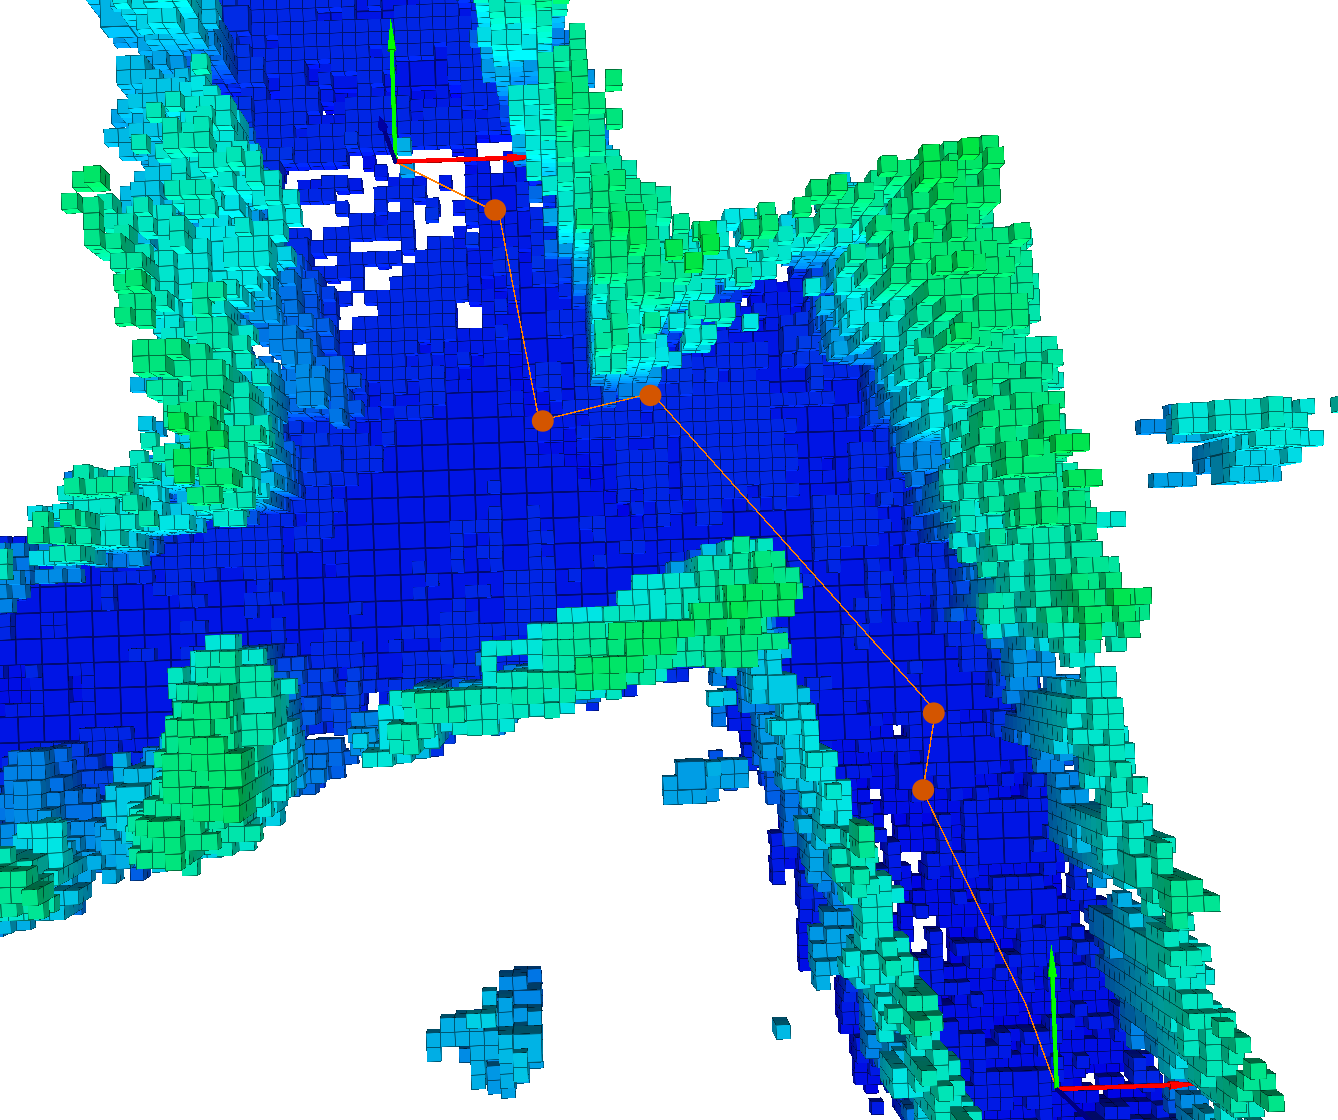
\includegraphics[trim = 50mm 0mm 30mm 0mm,clip,width=0.8\textwidth]{pics/smallGammaP.png}
   \caption{Straight line solution of the RRT algorithm with a fixed goal state. Start and goal state are each represented by a red $x$-vector and a green $y$-vector. The random sampled states are depicted as orange dots.}
   \label{pic:smallGamma}
\end{figure}



\section{RRT* Algorithm}\label{sec:RRTstar}

In contrast to the RRT algorithm the RRT* (or RRT Star) algorithm not only tries to connect to the nearest state in the tree but to several states near the sampled state. The user can define a threshold (on the distance) which defines which states of the tree belongs to the "near states". If there is no state within the user specified range the algorithm attempts to build a collision-free connection to the nearest state in the tree just as the RRT algorithm.  \newline
As a first step, the sampled state is connected to the best state among the near states whereas best means minimum cost/distance. Once the sampled state is added to the tree all the other states among the set of near states are connected to the sampled state. If the connection is collision-free and the cost of the total path is smaller than the cost of the existing path, the old path is replaced. \newline

An iteration of the RRT* algorithm can be depicted schematically:


\begin{enumerate}
  \item Generate a random sample
  \item A threshold defines a set of near states
  \item Try to build a collision-free connection to best state among the near states
  \item Add the sampled state and the connection to the tree 
  \item Try to connect all the other states from the set with the sampled state 
  \item Replace the old path if the new one has a smaller cost
  \item If there is no near state within the threshold apply the RRT algorithm
\end{enumerate}


Because the RRT* algorithm tries to connect to several states each iteration, the procedure to find a path takes longer and is computationally more expensive. However, solutions with lower cost can be found which is more important for most real life applications.

\subsection{Rewiring}

The sequence of step 5 and step 6 of the RRT* algorithm ("Try to connect all the other states from the set with the sampled state", "Replace the old path if the new one has a smaller cost") are called "rewiring". \newline 
The threshold which defines the set of near states depends on a user specified parameter $\gamma$. In this case, the threshold is the radius of a sphere, i.e. all the near states are located within this sphere. The radius $r$ can be calculated according to


\begin{equation}
r = \gamma * \left(\frac{ln(n+1)}{n+1}\right)^{1/d}
\label{equ:ballradius}
\end{equation}

where $n$ is the number of states which are already in the tree. The dimension of the state space $d$ is a fixed parameter and $ln$ represents the natural logarithm.\newline

As mention in section \ref{sec:RRTstar} the RRT* algorithm is computationally more expensive but returns trajectory with lower cost. Both aspects are caused by the rewiring and are therefore strongly influenced by the parameter $\gamma$. A large $\gamma$ defines a large sphere, hence it is likely to have more states (which are already in the tree) to be located within the sphere. The rewiring of the near states tends to result in shorter trajectories with fewer segments.

Figure \ref{pic:smallBBX} depicts the straight line solution of the RRT* algorithm with a fixed goal state. Compared to figure \ref{pic:smallGamma} a superior trajectory is found since a rewiring of the states in the tree was performed.

\begin{figure}[H]
   \centering
   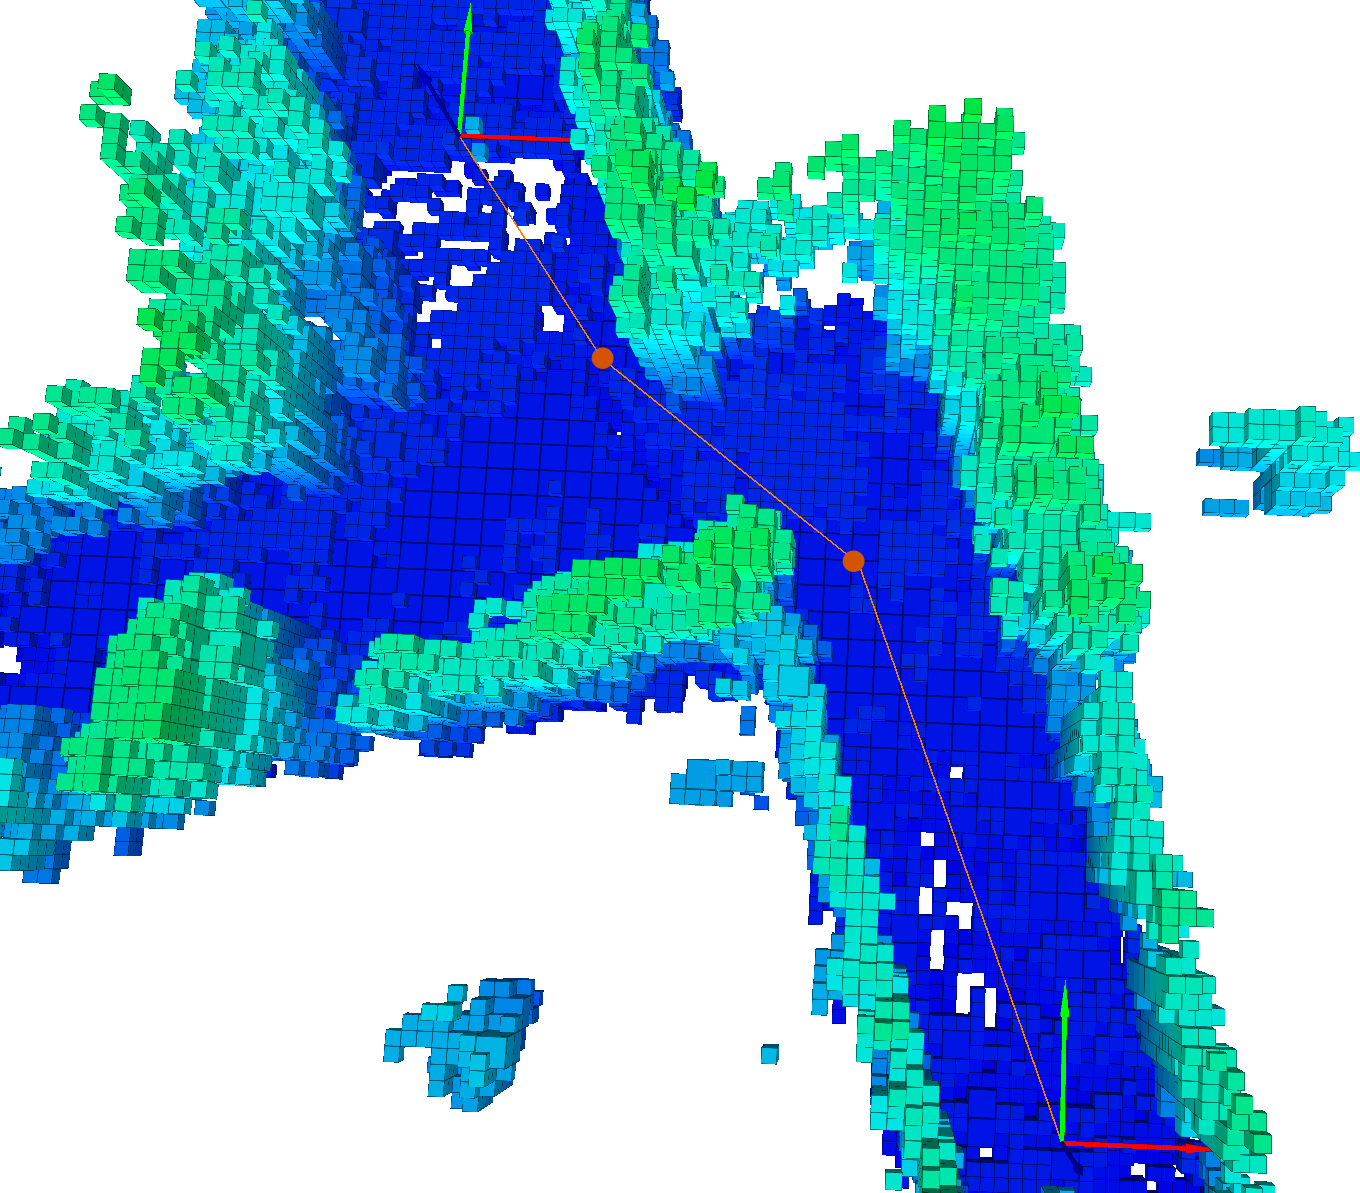
\includegraphics[trim = 50mm 0mm 30mm 0mm,clip,width=0.8\textwidth]{pics/smallBBXP.png}
   \caption{Straight line solution of the RRT* algorithm with a fixed goal state. Start and goal state are each represented by a red $x$-vector and a green $y$-vector. The random sampled states are depicted as orange dots. The $\gamma$ parameter in this example was set to $\gamma = 1.5$.}
   \label{pic:smallBBX}
\end{figure}


\subsection{Bounding Box}\label{sec:bbx}

The straight line solution in figure \ref{pic:smallBBX} is collision-free but passes by very close to the walls. In real life application not only a point mass but a object (in this master thesis a UAV) should follow the trajectory. Therefore a bounding box is installed around the trajectory. \newline
The bounding box is implemented as a cuboid. The 3 dimension of the cuboid can be defined individually. The trajectory is then divided into a discrete trajectory and the bounding box is installed around the discrete points. If there is a obstacle in one of the bounding boxes the hole straight line is considered as  in collision. \newline

Figure \ref{pic:bbx} depicts the straight line solution of the RRT* algorithm with a bounding box. In contrast to figure \ref{pic:smallBBX} the trajectory is now located more central in the hallway because the bounding box makes it impossible to pass by the wall very close. Because the trajectory proceeds less direct from start to goal state the total distance of the trajectory increases. 

\begin{figure}[H]
   \centering
   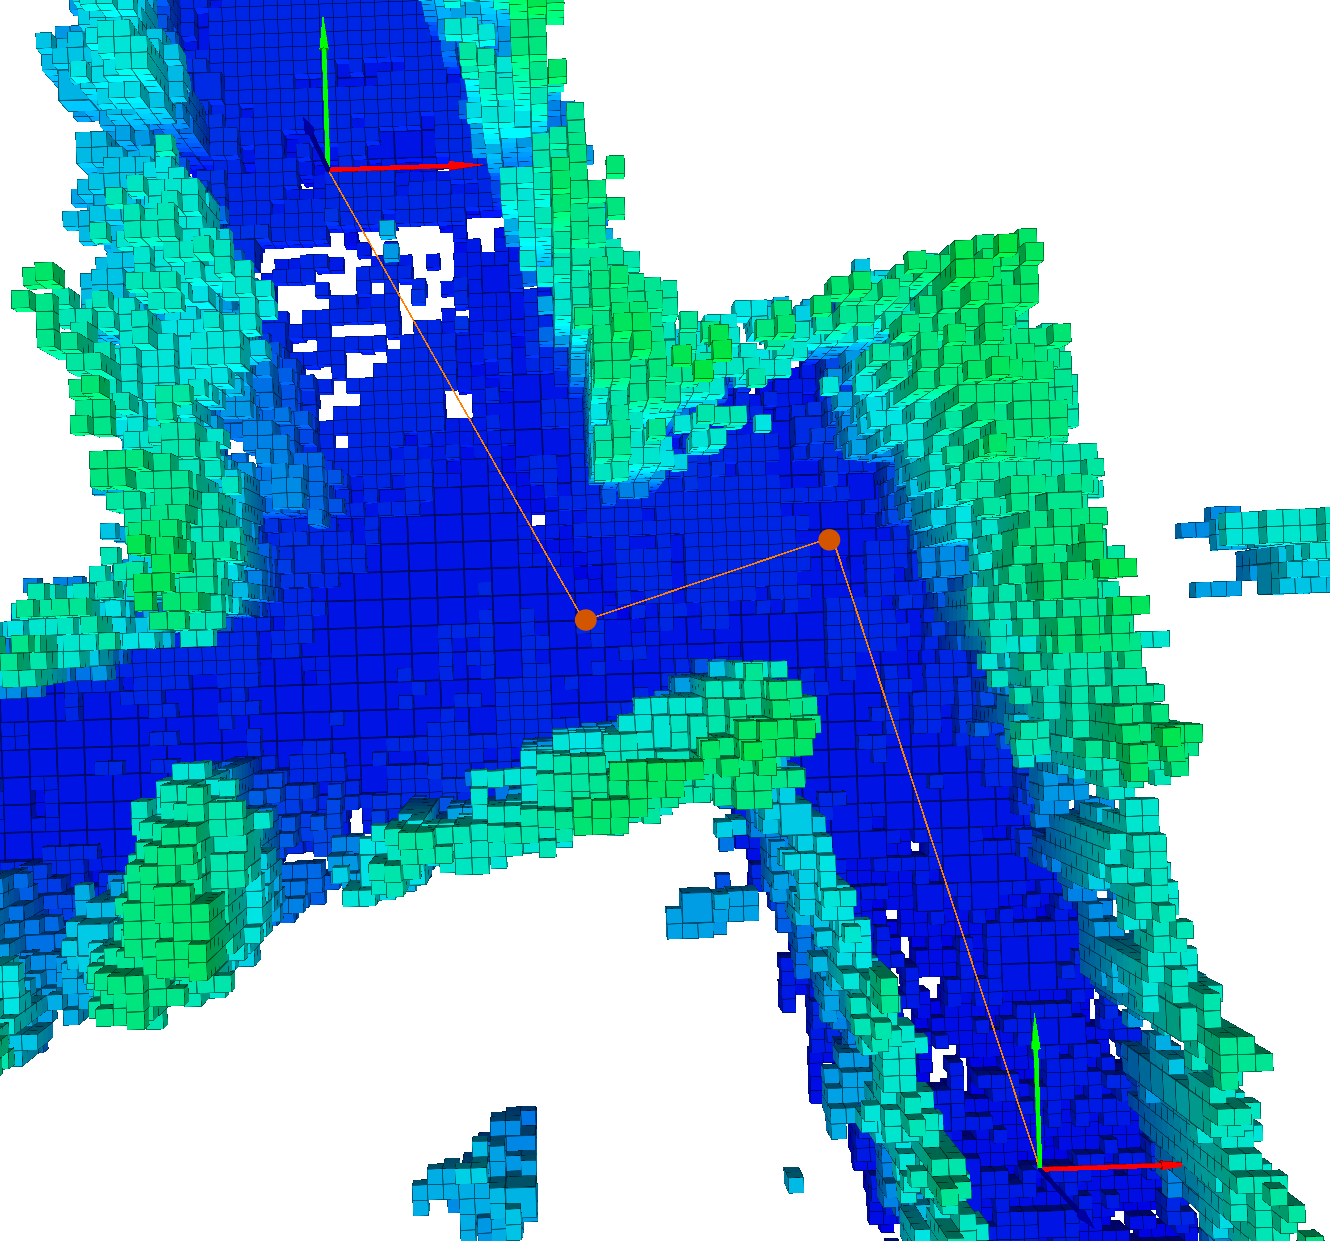
\includegraphics[trim = 50mm 0mm 30mm 0mm,clip,width=0.8\textwidth]{pics/largeBBXP.png}
   \caption{Straight line solution of the RRT* algorithm with bounding box. Due to the bounding box the trajectory is located more central in the hallway because the bounding box makes it impossible to pass by the wall very close. The $\gamma$ parameter in this example was set to $\gamma = 1.5$.}
   \label{pic:bbx}
\end{figure}

\subsection{Ray Check}

 TODO: verbindung zu Octompa
 
 matlab figure



%\begin{figure}[h]
%   \centering
%   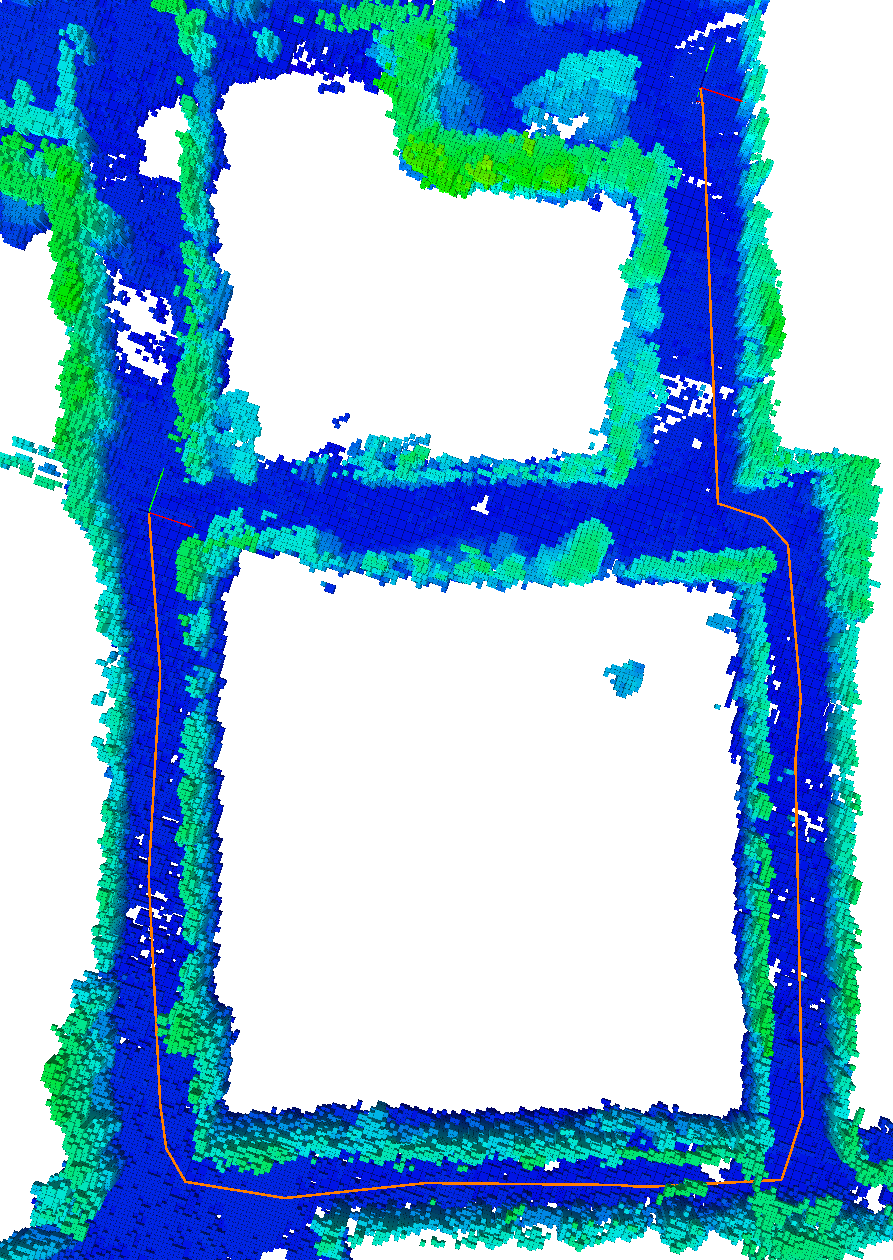
\includegraphics[width=1\textwidth]{pics/MapLine.png}
%   \caption{Ein Bild.}
%\end{figure}



%\begin{figure}[h]
%   \centering
%   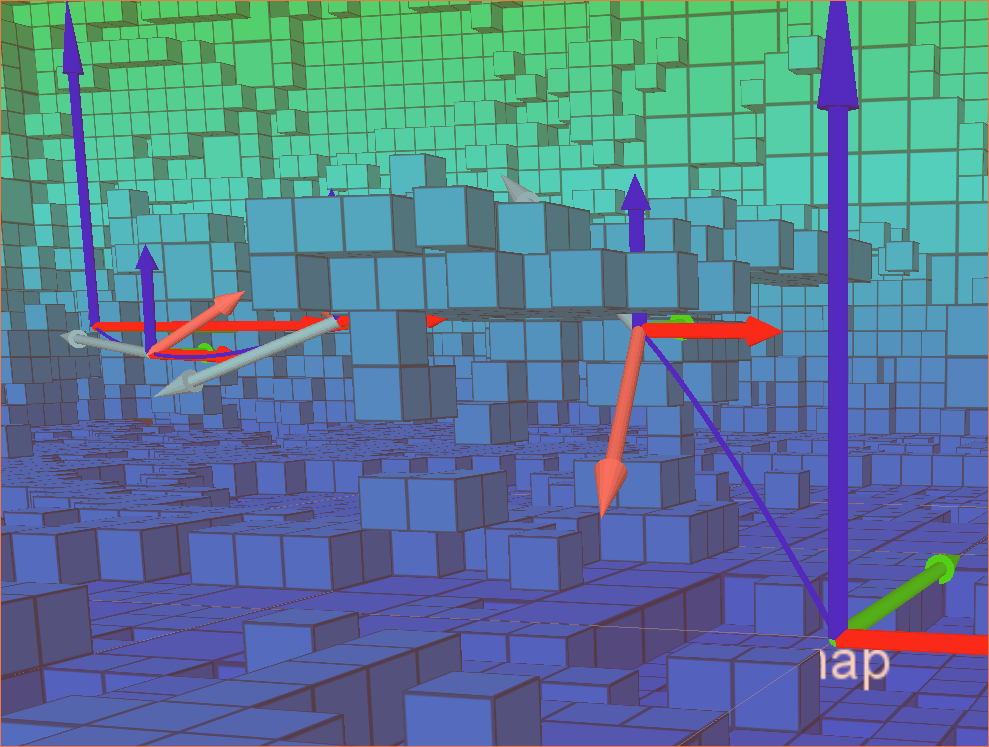
\includegraphics[width=1\textwidth]{pics/initialSolution.png}
%   \caption{Ein Bild.}
%\end{figure}
%
%
%\begin{figure}[h]
%   \centering
%   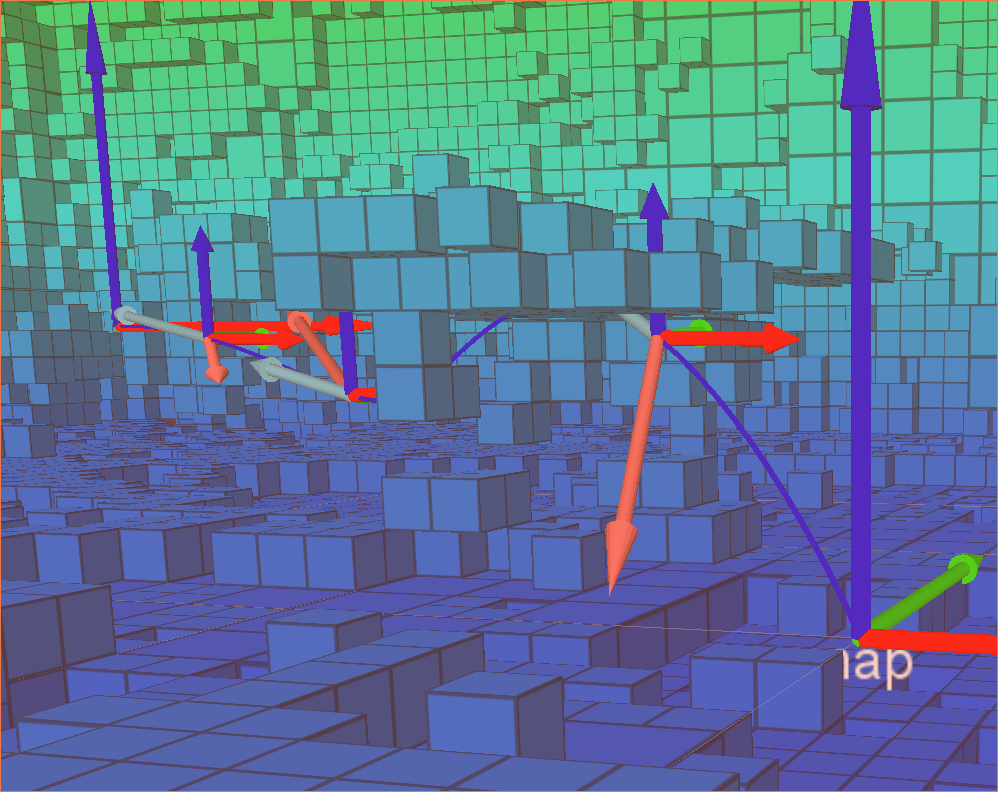
\includegraphics[width=1\textwidth]{pics/Vertex_in_middle_2.png}
%   \caption{Ein Bild.}
%\end{figure}
%
%\begin{figure}[h]
%   \centering
%   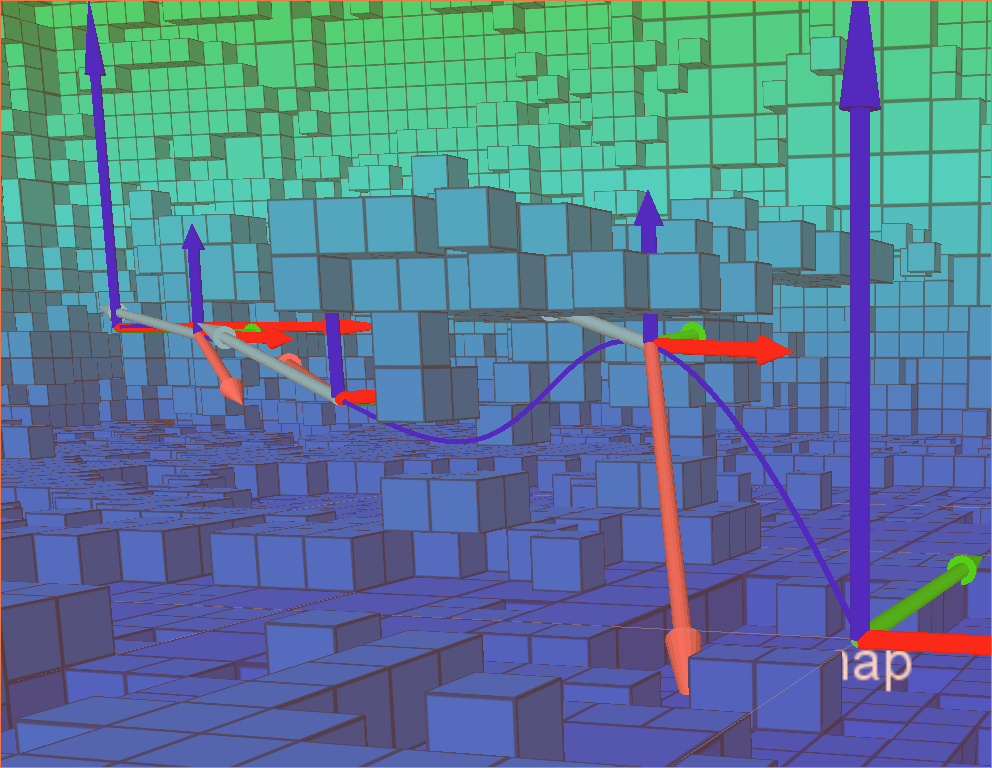
\includegraphics[width=1\textwidth]{pics/section.png}
%   \caption{Ein Bild.}
%\end{figure}
%
%
%\begin{figure}[h]
%   \centering
%   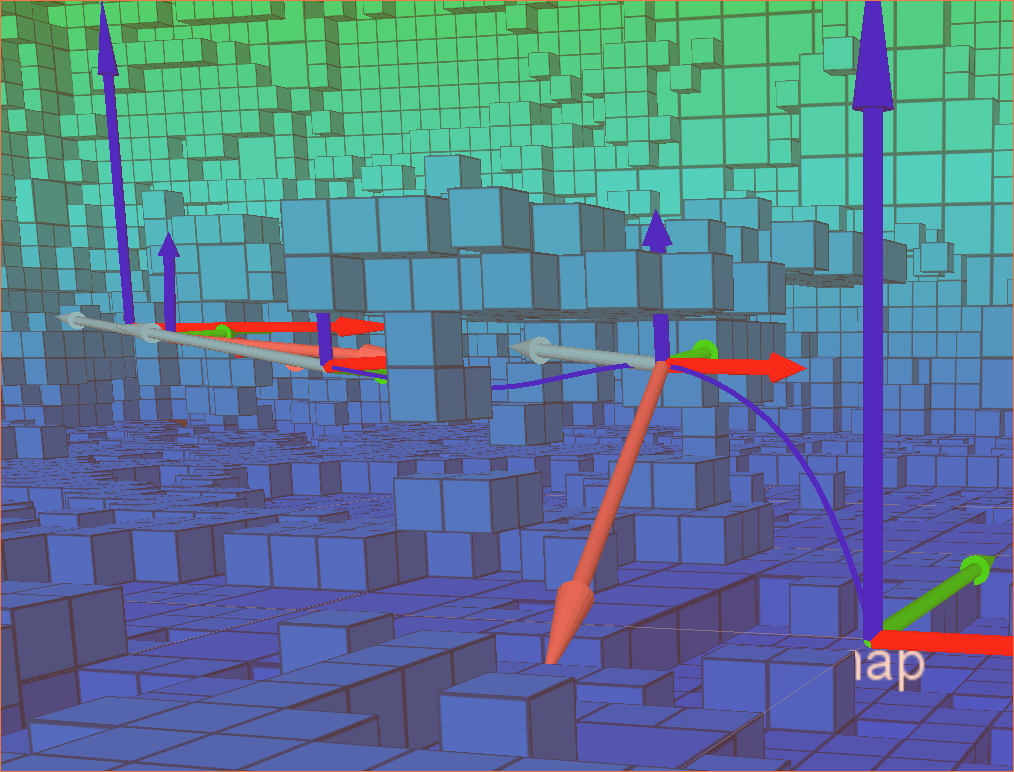
\includegraphics[width=1\textwidth]{pics/Nlopt_after_sectionAndTime.png}
%   \caption{Ein Bild.}
%\end{figure}
 \cleardoublepage
 %
\chapter{Einige wichtige Hinweise zum Arbeiten mit \LaTeX\ }\label{sec:latexumg}

Nachfolgend wird die Codierung einiger oft verwendeten Elemente
kurz beschrieben. Das Einbinden von Bildern ist in \LaTeX\ nicht
ganz unproblematisch und h�ngt auch stark vom verwendeten Compiler
ab. Typisches Format f�r Bilder in \LaTeX\ ist
EPS\footnote{Encapsulated Postscript}.


\section{Gliederungen}\label{sec:gliederung}

Ein Text kann mit den Befehlen \texttt{\textbackslash
chapter\{.\}}, \texttt{\textbackslash section\{.\}},
\texttt{\textbackslash subsection\{.\}} und \texttt{\textbackslash
subsubsection\{.\}} gegliedert werden.


\section{Referenzen und Verweise}\label{sec:refverw}

Literaturreferenzen werden mit dem Befehl \texttt{\textbackslash
cite\{.\}} erzeugt. Ein Beispiel: \cite{comfilt}.

Zur Erzeugung von Fussnoten wird der Befehl \texttt{\textbackslash
footnote\{.\}} verwendet. Auch hier ein Beispiel\footnote{Bla
bla.}.

Querverweise im Text werden mit \texttt{\textbackslash label\{.\}}
verankert und mit \texttt{\textbackslash ref\{.\}} erzeugt.
Beispiel einer Referenz auf das zweite Kapitel:
Kapitel~\ref{sec:latexumg}.


\section{Aufz�hlungen}\label{sec:aufz}

Folgendes Beispiel einer Aufz�hlung ohne Numerierung,
\begin{itemize}
  \item Punkt 1
  \item Punkt 2
\end{itemize}
wurde erzeugt mit:
\begin{verbatim}
\begin{itemize}
  \item Punkt 1
  \item Punkt 2
\end{itemize}
\end{verbatim}

Folgendes Beispiel einer Aufz�hlung mit Numerierung,
\begin{enumerate}
  \item Punkt 1
  \item Punkt 2
\end{enumerate}
wurde erzeugt mit:
\begin{verbatim}
\begin{enumerate}
  \item Punkt 1
  \item Punkt 2
\end{enumerate}
\end{verbatim}

Folgendes Beispiel einer Auflistung,
\begin{description}
  \item[P1] Punkt 1
  \item[P2] Punkt 2
\end{description}
wurde erzeugt mit:
\begin{verbatim}
\begin{description}
  \item[P1] Punkt 1
  \item[P2] Punkt 2
\end{description}
\end{verbatim}


\section{Erstellen einer Tabelle}\label{sec:tabellen}

Ein Beispiel einer Tabelle:
\begin{table}[h]
\begin{center}
 \caption{Daten der Fahrzyklen ECE, EUDC, NEFZ.}\vspace{1ex}
 \label{tab:tabnefz}
 \begin{tabular}{ll|ccc}
 \hline
 Kennzahl & Einheit & ECE & EUDC & NEFZ \\ \hline \hline
 Dauer & s & 780 & 400 & 1180 \\
 Distanz & km & 4.052 & 6.955 & 11.007 \\
 Durchschnittsgeschwindigkeit & km/h & 18.7 &  62.6 & 33.6 \\
 Leerlaufanteil & \% & 36 & 10 & 27 \\
 \hline
 \end{tabular}
\end{center}
\end{table}

Die Tabelle wurde erzeugt mit:
\begin{verbatim}
\begin{table}[h]
\begin{center}
 \caption{Daten der Fahrzyklen ECE, EUDC, NEFZ.}\vspace{1ex}
 \label{tab:tabnefz}
 \begin{tabular}{ll|ccc}
 \hline
 Kennzahl & Einheit & ECE & EUDC & NEFZ \\ \hline \hline
 Dauer & s & 780 & 400 & 1180 \\
 Distanz & km & 4.052 & 6.955 & 11.007 \\
 Durchschnittsgeschwindigkeit & km/h & 18.7 &  62.6 & 33.6 \\
 Leerlaufanteil & \% & 36 & 10 & 27 \\
 \hline
 \end{tabular}
\end{center}
\end{table}
\end{verbatim}


\section{Einbinden einer EPS-Graphik}\label{sec:epsgraph}

Das Einbinden von Graphiken kann wie folgt bewerkstelligt werden:
\begin{verbatim}
\begin{figure}[h]
   \centering
   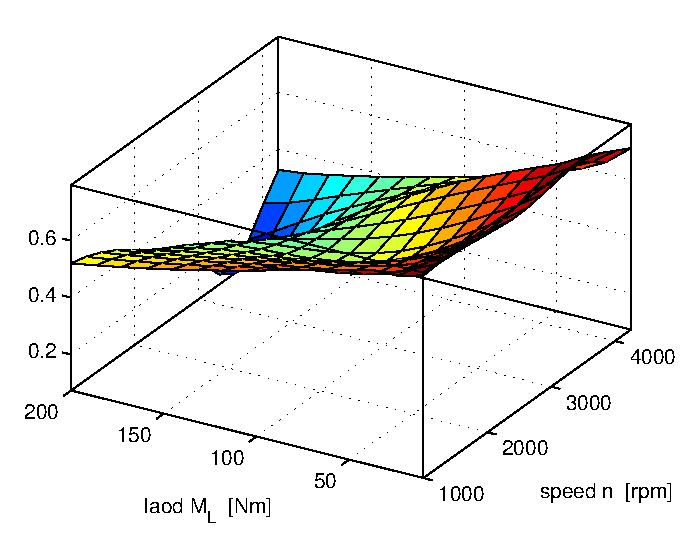
\includegraphics[width=0.75\textwidth]{pics/k_surf.eps}
   \caption{Ein Bild.}
   \label{pics:k_surf}
\end{figure}
\end{verbatim}

\begin{figure}[h]
   \centering
   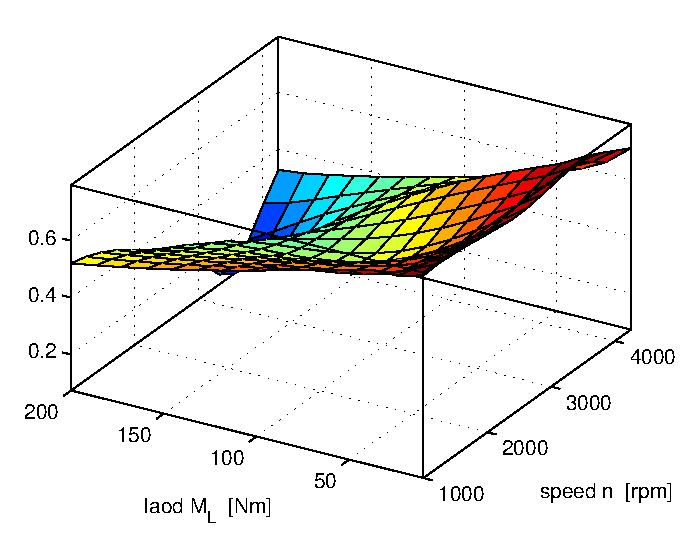
\includegraphics[width=0.75\textwidth]{pics/k_surf.eps}
   \caption{Ein Bild.}
   \label{pics:k_surf}
\end{figure}

oder bei zwei Bildern nebeneinander mit:
\begin{verbatim}
\begin{figure}[h]
  \begin{minipage}[t]{0.48\textwidth}
    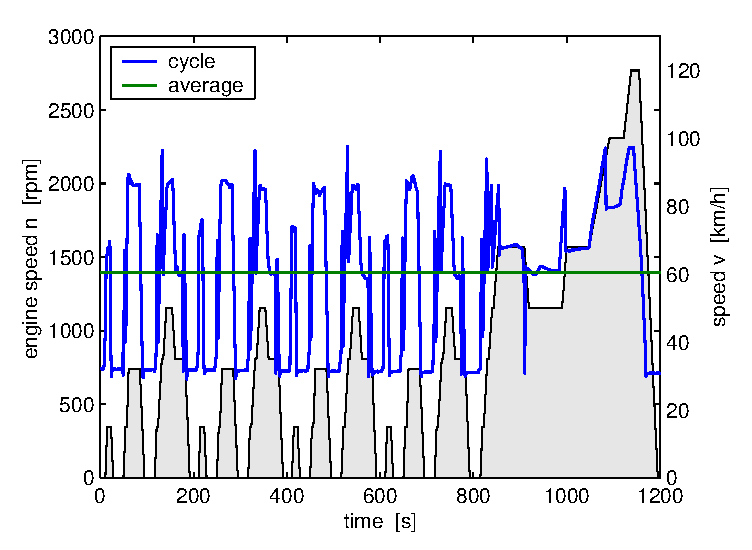
\includegraphics[width = \textwidth]{pics/cycle_we.eps}
  \end{minipage}
  \hfill
  \begin{minipage}[t]{0.48\textwidth}
    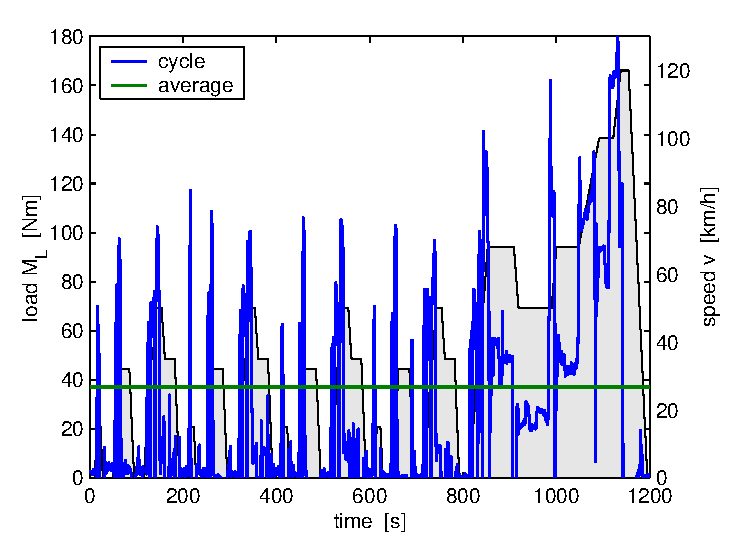
\includegraphics[width = \textwidth]{pics/cycle_ml.eps}
  \end{minipage}
  \caption{Zwei Bilder nebeneinander.}
  \label{pics:cycle}
\end{figure}
\end{verbatim}

\begin{figure}[h]
  \begin{minipage}[t]{0.48\textwidth}
    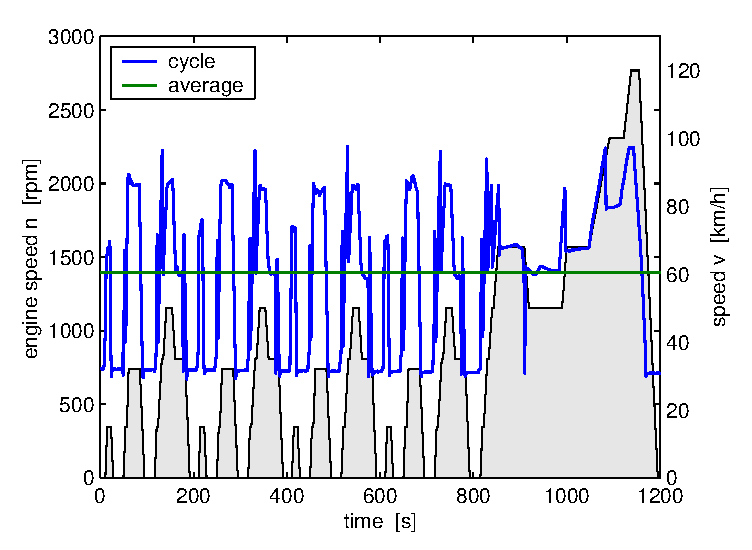
\includegraphics[width = \textwidth]{pics/cycle_we.eps}
  \end{minipage}
  \hfill
  \begin{minipage}[t]{0.48\textwidth}
    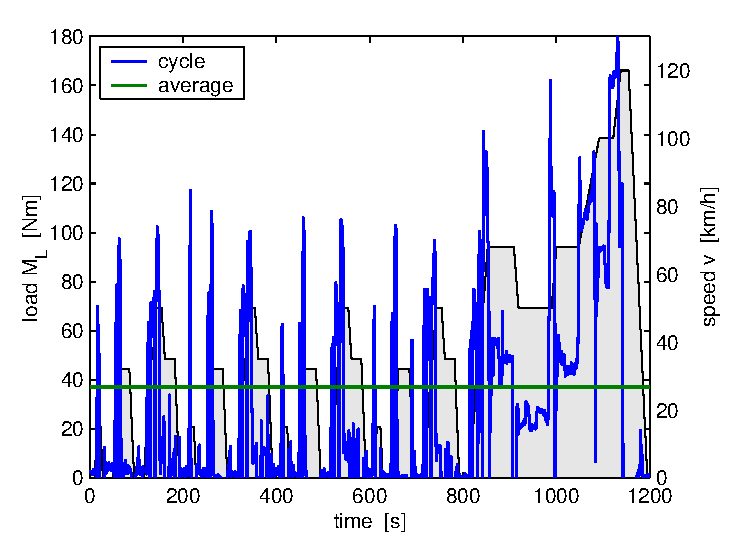
\includegraphics[width = \textwidth]{pics/cycle_ml.eps}
  \end{minipage}
  \caption{Zwei Bilder nebeneinander.}
  \label{pics:cycle}
\end{figure}

Bemerkung: Ersetzt man den Positionierungsparameter \texttt{h}
durch \texttt{H}, so wird das Gleiten der Abbildung verhindert.


\section{Mathematische Formeln}\label{sec:math}

Einfache mathematische Formeln werden mit der equation-Umgebung
erzeugt:
\begin{equation}
 p_{me0f}(T_e,\omega_e) \ = \ k_1(T_e) \cdot (k_2+k_3 S^2
 \omega_e^2) \cdot \Pi_{max} \cdot \sqrt{\frac{k_4}{B}} \, .
\end{equation}

Der Code dazu lautet:
\begin{verbatim}
\begin{equation}
 p_{me0f}(T_e,\omega_e) \ = \ k_1(T_e) \cdot (k_2+k_3 S^2
 \omega_e^2) \cdot \Pi_{max} \cdot \sqrt{\frac{k_4}{B}} \, .
\end{equation}
\end{verbatim}

Mathematische Ausdr�cke im Text werden mit \$formel\$ erzeugt (zB:
$a^2+b^2=c^2$).


\section{Weitere n�tzliche Befehle}\label{sec:div}

Hervorhebungen im Text sehen so aus: \emph{hervorgehoben}. Erzeugt
werden sie mit dem \texttt{\textbackslash epmh\{.\}} Befehl.

 %\cleardoublepage
% \include{}
% \cleardoublepage
% \include{}
% \cleardoublepage
% ...
%
%---------------------------------------------------------------------------
% Appendix

 \appendix
 
\chapter{Irgendwas}\label{sec:irgendwas}

Bla bla \dots

 \cleardoublepage

%
%\chapter{Nochmals irgendwas}\label{sec:nochirgendwas}
%
%Bla bla \dots
%
% \cleardoublepage

%
%---------------------------------------------------------------------------
% Literature

 
\begin{thebibliography}{99}
%\addcontentsline{toc}{chapter}{Literaturverzeichnis}
\addcontentsline{toc}{chapter}{Bibliography}



\bibitem {he} {\sc R. He, A. Bachrach, M. Achtelik, A. Geramifard, D. Gurdan, S. Prentice,
J. Stumpf, and N. Roy}: 
{\it On the design and use of a micro air
vehicle to track and avoid adversaries}. The Int. Journal of Robotics
Research, vol. 29, pp. 529-546, 2010.


\bibitem {colling} {\sc D. Colling, O. A.~Yakimenko, J. F.~Whidborne, and A. K.~Cooke}:
{\it A prototype of an autonomous controller for a quadrotor UAV}. In
Proceedings of the European Control Conference, Kos, Greece, 2007,
pp. 1-8.


\bibitem {hehn} {\sc M. Hehn and R. D'Andrea }:
{\it Quadrocopter trajectory generation and control}. In
International Federation of Automatic Control (IFAC), World Congress 2011, 2011.


\bibitem {lup} {\sc S. Lupashin, A. Schollig, M. Sherback, and R. D'Andrea}:
 {\it A simple learning strategy for high-speed quadrocopter multi-flips}.
In Proc. of the IEEE Int. Conf. on Robotics and Automation, Anchorage, AK,
May 2010, pp. 1642-1648.


\bibitem {bou} {\sc Y. Bouktir, M. Haddad, and T. Chettibi}:
{\it Trajectory Planning for a
Quadrotor Helicopter}. In Mediterranean Conference on Control and
Automation, Jun. 2008, pp. 1258-1263


\bibitem {mellinger} {\sc D. Mellinger and V. Kumar}: 
{\it Minimum snap trajectory generation and
control for quadrotors}. In International Conference on Robotics and
Automation, 2011, pp. 2520-2525.

\bibitem {lik} {\sc M. Likhachev, G. Gordon and S. Thrun}: 
{\it  ARA*: Anytime A* with Provable Bounds on Sub-Optimality }.
Advances in Neural Information
Processing Systems, vol. 16, 2003

\bibitem {richter} {\sc C. Richter,  A. Bry, and N, Roy}: 
{\it  Polynomial Trajectory Planning
for Quadrotor Flight}.
In International Conference on Robotics and
Automation, 2013.



\end{thebibliography}


%---------------------------------------------------------------------------

\end{document}
%===========================================================================
